\documentclass[10pt]{article}
\usepackage[margin=1in]{geometry}
 \usepackage{auto-pst-pdf}
\usepackage{graphicx}
\usepackage{footnote}
%\usepackage{arydshln}
\usepackage{ifpdf}
\ifpdf
  \usepackage{epstopdf}
\fi
\usepackage{multirow}
\usepackage{epsfig}
\usepackage{float}
\usepackage{url}
\usepackage{color}
\usepackage{subfigure}

%\newcommand\solidrule[1][1cm]{\rule[0.5ex]{#1}{.4pt}}
%\newcommand\dashedrule{\mbox{%
%  \solidrule[2mm]\hspace{2mm}\solidrule[2mm]\hspace{2mm}\solidrule[2mm]}}
  
%\usepackage{hyperref}

\begin{document}
\title{Repeatability Test}

\author{
Young-Kyoon Suh\\ 
Data-Intensive Systems Lab \\
School of Computer Science \& Engineering\\
Kyungpook National University
}
\maketitle

\section{Description}
This document characterizes execution times 
measured on a simple program in pure-computation mode, called {\em INC}, 
with increasing task lengths (up to 16,384 seconds from 1 second). 
For the characterization, we present various histograms of INC throughout this document.
The main goal of examining these histograms is to make sure if 
two (or more) histograms of INC with the same task length 
have the same shape or not. If that's the case, then we can say that such an INC run is so called {\em repeatable}; 
in other words, {\em repeatability} is satisfied in our experimental settings. 
Another goal is to uncover and explicate several interesting structures behind the histograms. 
The third goal is to build a statistical distribution (or model) fitting in the histograms, so that later we 
are capable of predicting a concrete execution time via 
the model on an arbitrary algorithm with a given input on a real execution environment.

In our experiments, we used EMPv5~\cite{EMP}. 
(That said, the second step of EMPv5 was on purpose omitted, just to obtain better histograms by retaining more samples.) 
In the protocol, we use taskstats C struct to get measures of a captured process. 
The taskstat's data is delivered via a netlink socket from the kernel space. 
The receive buffer for the socket is not robust for many observed processes~\cite{Metrology}. 
Fortunately, there is an average of 95 processes per iteration of a run, 
which turns out to be fine with the struct. 
For a much more number of processes, 
the use of  {\tt /proc/}[pid]{\tt{/stat}} is preferred, 
as (i) there are equivalent measures available in the {\tt /proc} filesystem, 
and (ii) there's little constraint on the use as opposed to taskstats. 

Now we show histograms of elapsed time (ET) and process time (PT) of INC via the EMPv5 protocol.

\pagebreak

\section{Histograms on the First Run~\label{sec:first_run}} 
This section exhibits histograms on the first run of 
INC with its task length increasing from 1 second to 4,096 seconds. 
The detailed description of the base data is from Table~\ref{tab:exp_notes1}.

%\section{Experiment Notes}
\paragraph{Experiment Notes:}
Table~\ref{tab:exp_notes1} provides a short description of our experimental runs, 
on which the following histograms are based.

%% done
\begin{table}[h]
\begin{center}
\begin{tabular}{|p{3cm}|p{2cm}|p{3cm}|p{4cm}|p{3cm}|} \hline
Machine & Task Length (sec) & Description & Experiment Period & Relevant \linebreak Histograms\\ \hline
{\tt sodb9} (plugged into {\em the upper left} power strip)  &  INC1$\sim$INC64 & 1000 samples, each & 2017-03-02 $\sim$ 2017-03-04 & Figs.~\ref{fig:s9_r1_et_hist1},~\ref{fig:s9_r1_et_hist2},~\ref{fig:s9_r1_pt_hist1}, and~\ref{fig:s9_r1_pt_hist2}\\ \hline

{\tt sodb9} (plugged into {\em the upper left} power strip) &  INC19, INC20, INC21.125, INC60, INC62, INC224 & 1000 samples, each, applied by EMPv4 & 2017-05-31, 2018-12-03, 2019-03-04 $\sim$ 2019-03-14 & Figs.~\ref{fig:s9_r1_pt_hist2},~\ref{fig:s9_r1_pt_hist2-2}, and~\ref{fig:inc224_v4}\\ \hline

{\tt sodb9} (plugged into {\em the upper left} power strip)  &  INC128$\sim$ INC1024 & 300 samples, each & 2017-03-04 $\sim$ 2017-03-11 & 
Figs.~\ref{fig:s9_r1_et_hist3},~\ref{fig:s9_r1_pt_hist3}, and~\ref{fig:s9_r1_pt_hist4}\\ \hline

{\tt sodb10} (plugged into {\em the upper left} power strip)  & INC2048 & 300 samples & 2017-03-02 $\sim$ 2017-03-09 & Figs.~\ref{fig:inc2048_r1_et_hist_v5} and~\ref{fig:inc2048_r1_hist_v5}\\ \hline
{\tt sodb12} (plugged into {\em the upper right} power strip)  & INC4096 & 300 samples & 2017-02-13 $\sim$ 2017-02-27 & Figs.~\ref{fig:inc4096_r1_et_hist_v5} and~\ref{fig:inc4096_r1_hist_v5}\\ \hline
\end{tabular}
\end{center}
\vspace{-.2in}
\caption{Notes on experiment runs used for histograms\label{tab:exp_notes1}}
\end{table}

\pagebreak

\subsection{ET}

\begin{figure}[hp!]
	\centering
	\subfigure[ET frequency on INC1 on {\tt sodb9}]{
		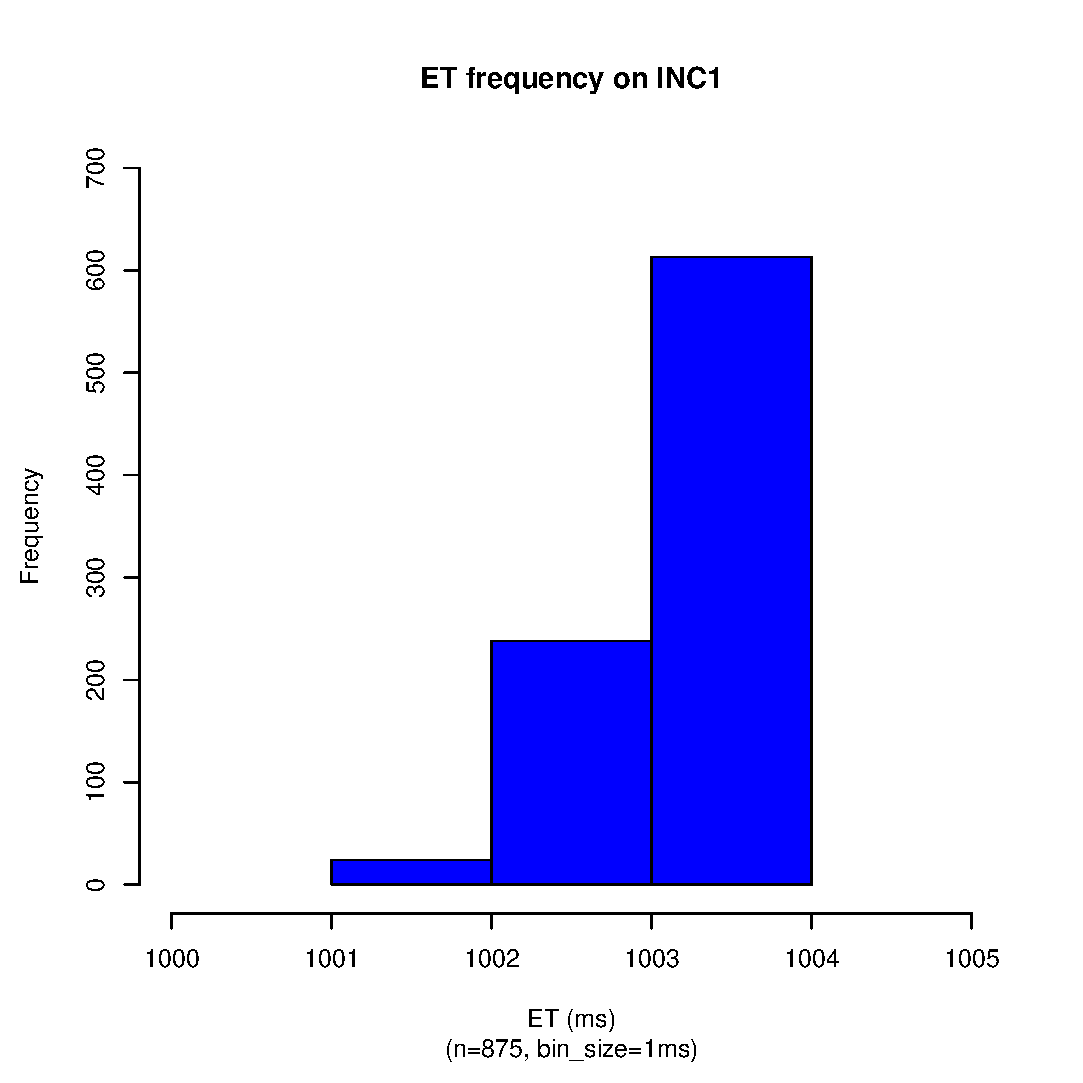
\includegraphics[scale=0.43]{repet_data1/1_sec_et_hist_v5.eps}
		\label{fig:inc1_r1_et_hist_v5}
	}
	\subfigure[ET frequency on INC2 on {\tt sodb9}]{
		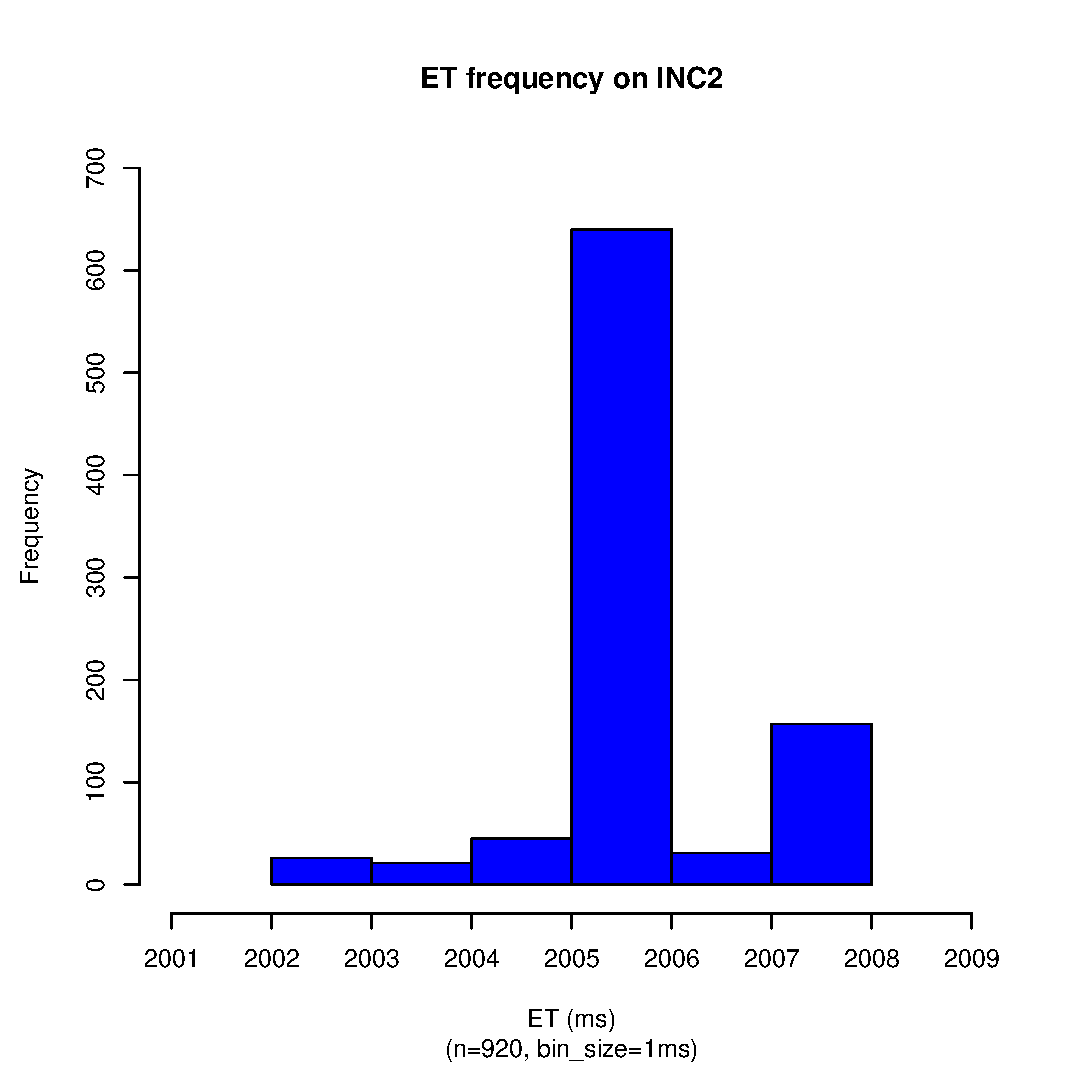
\includegraphics[scale=0.43]{repet_data1/2_sec_et_hist_v5.eps}
		\label{fig:inc2_r1_et_hist_v5}
	}
	\subfigure[ET frequency on INC4 on {\tt sodb9}]{
		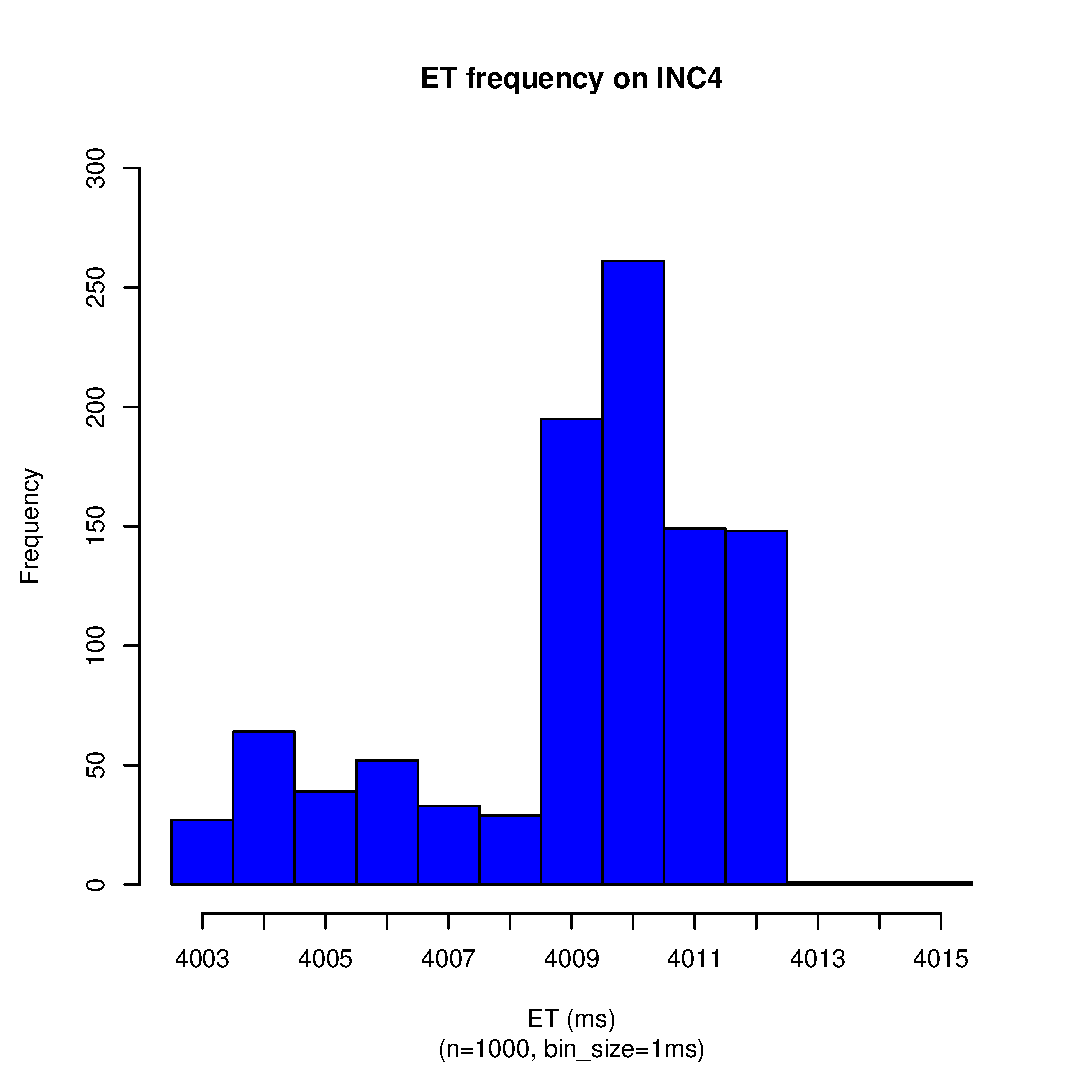
\includegraphics[scale=0.43]{repet_data1/4_sec_et_hist_v5.eps}
		\label{fig:inc4_r1_et_hist_v5}
	}
	\subfigure[ET frequency on INC8 on {\tt sodb9}]{
		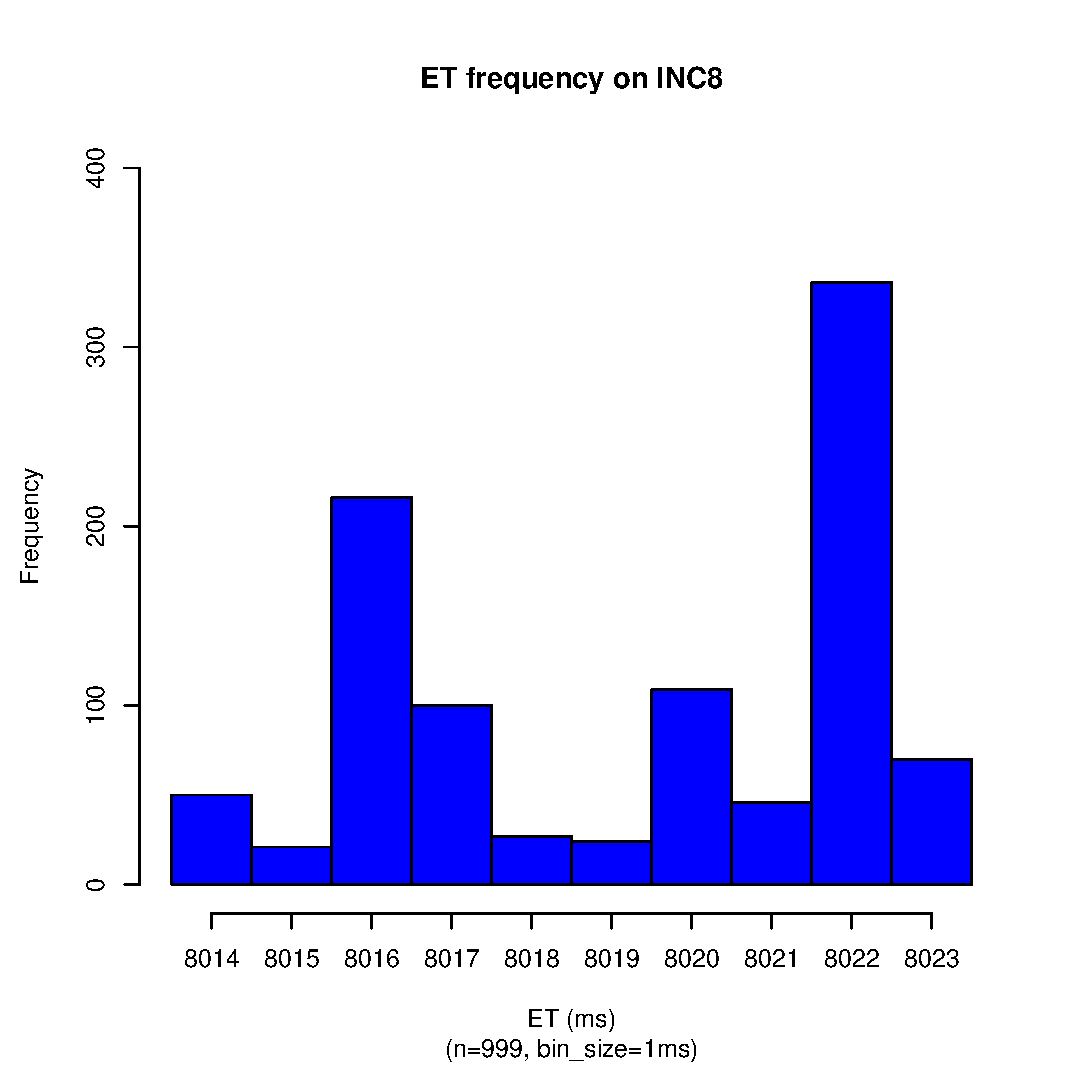
\includegraphics[scale=0.43]{repet_data1/8_sec_et_hist_v5.eps}
		\label{fig:inc8_r1_et_hist_v5}
	}
	\caption{ET Histograms of INC1 ... INC8~\label{fig:s9_r1_et_hist1}}
\end{figure}

\begin{figure}[hp!]
	\centering
	\subfigure[ET frequency on INC16 on {\tt sodb9}]{
		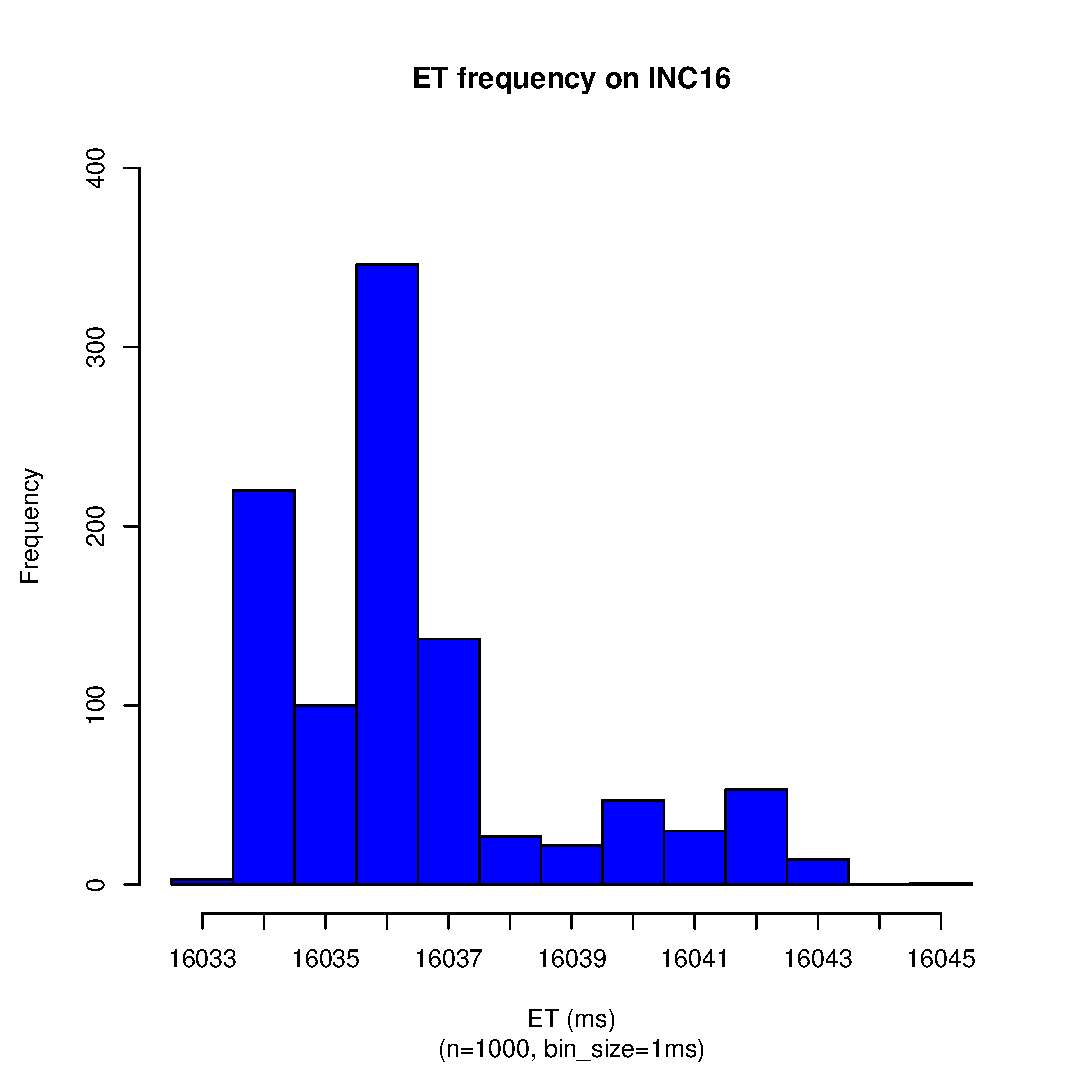
\includegraphics[scale=0.43]{repet_data1/16_sec_et_hist_v5.eps}
		\label{fig:inc16_r1_et_hist_v5}
	}
	\subfigure[ET frequency on INC32 on {\tt sodb9}]{
		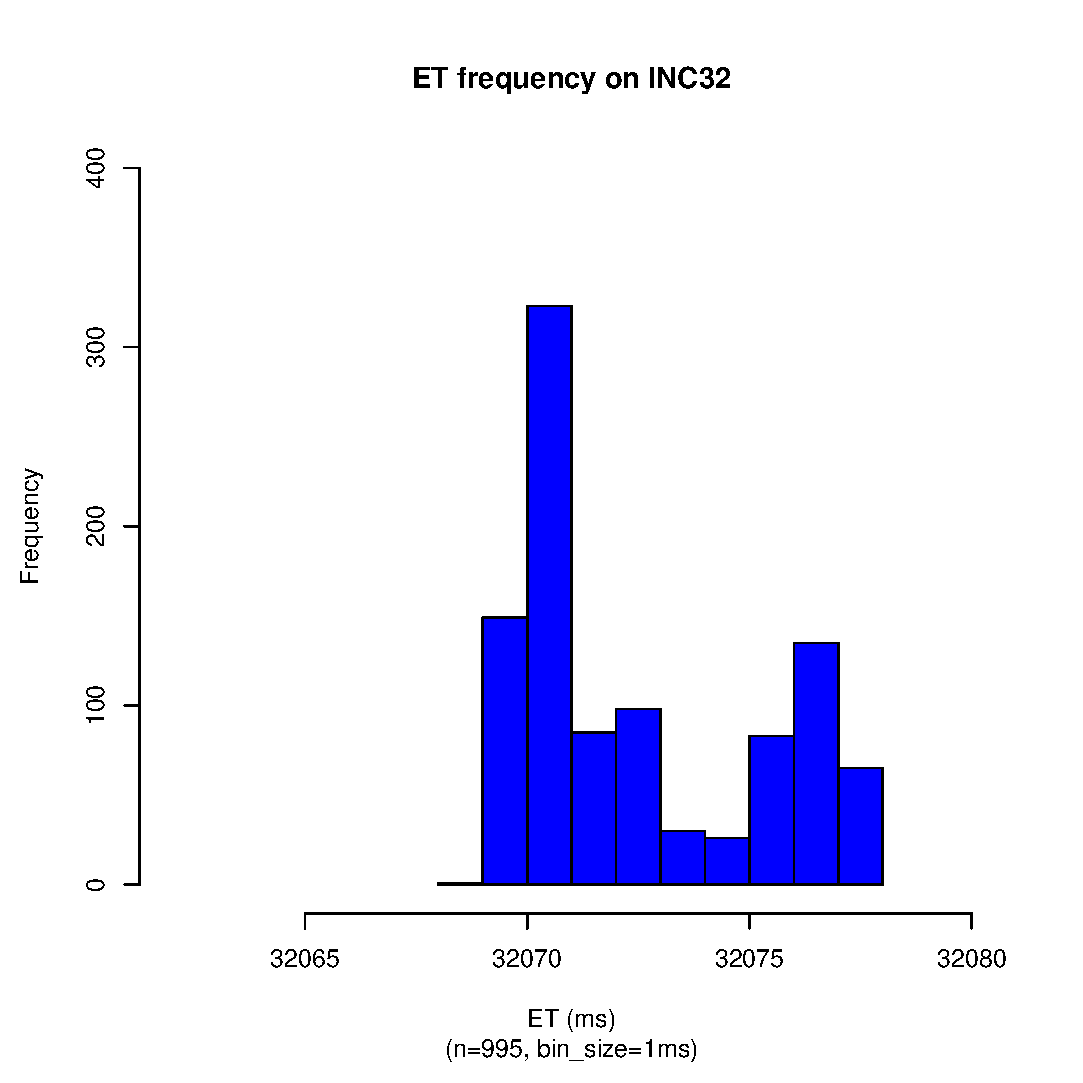
\includegraphics[scale=0.43]{repet_data1/32_sec_et_hist_v5.eps}
		\label{fig:inc32_r1_et_hist_v5}
	}
	\subfigure[ET frequency on INC64 on {\tt sodb9}]{
		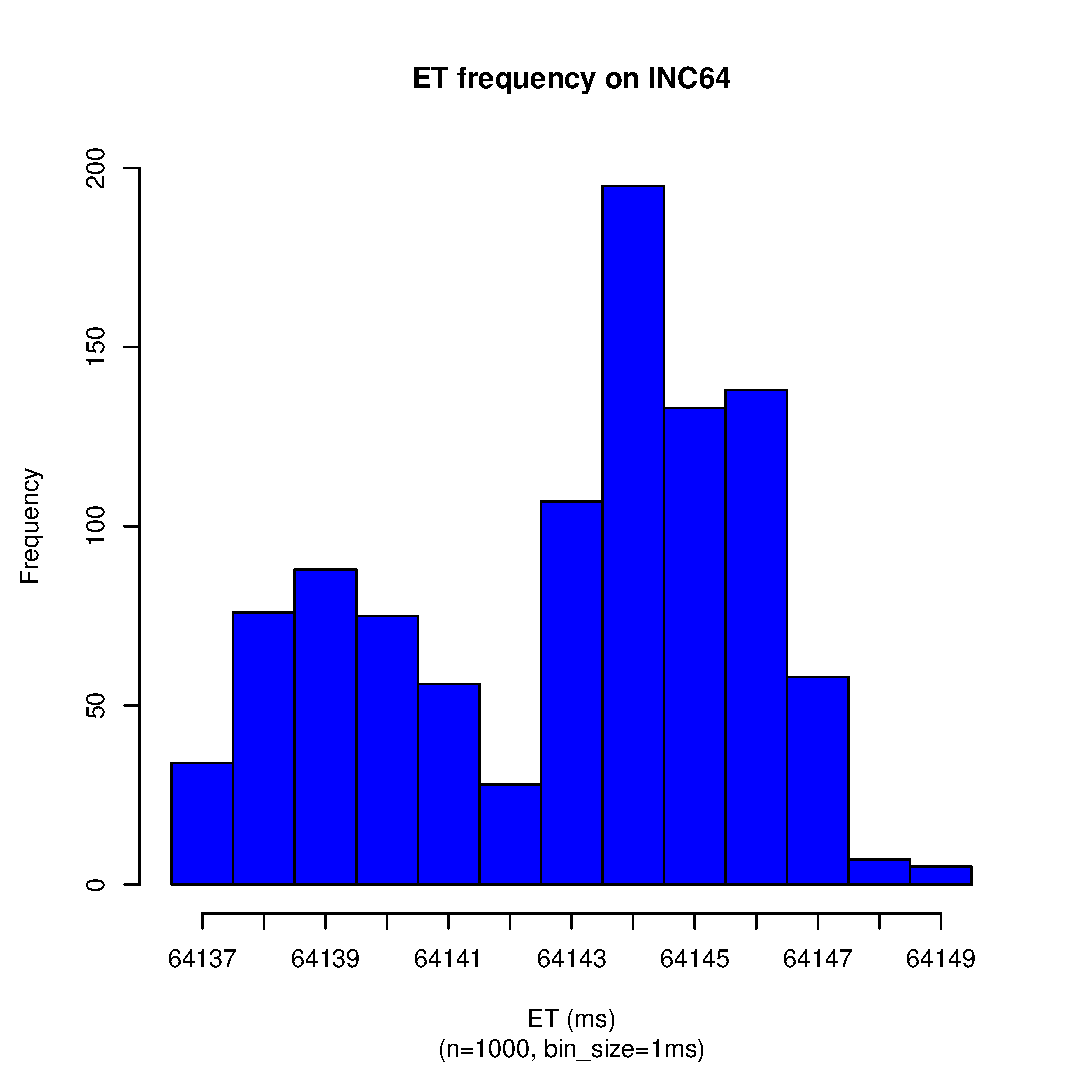
\includegraphics[scale=0.43]{repet_data1/64_sec_et_hist_v5.eps}
		\label{fig:inc64_r1_et_hist_v5}
	}
	\caption{ET Histograms of INC16 ... INC64~\label{fig:s9_r1_et_hist2}}
\end{figure}

\begin{figure}[hp!]
	\centering
	\subfigure[ET frequency on INC128 on {\tt sodb9}]{
		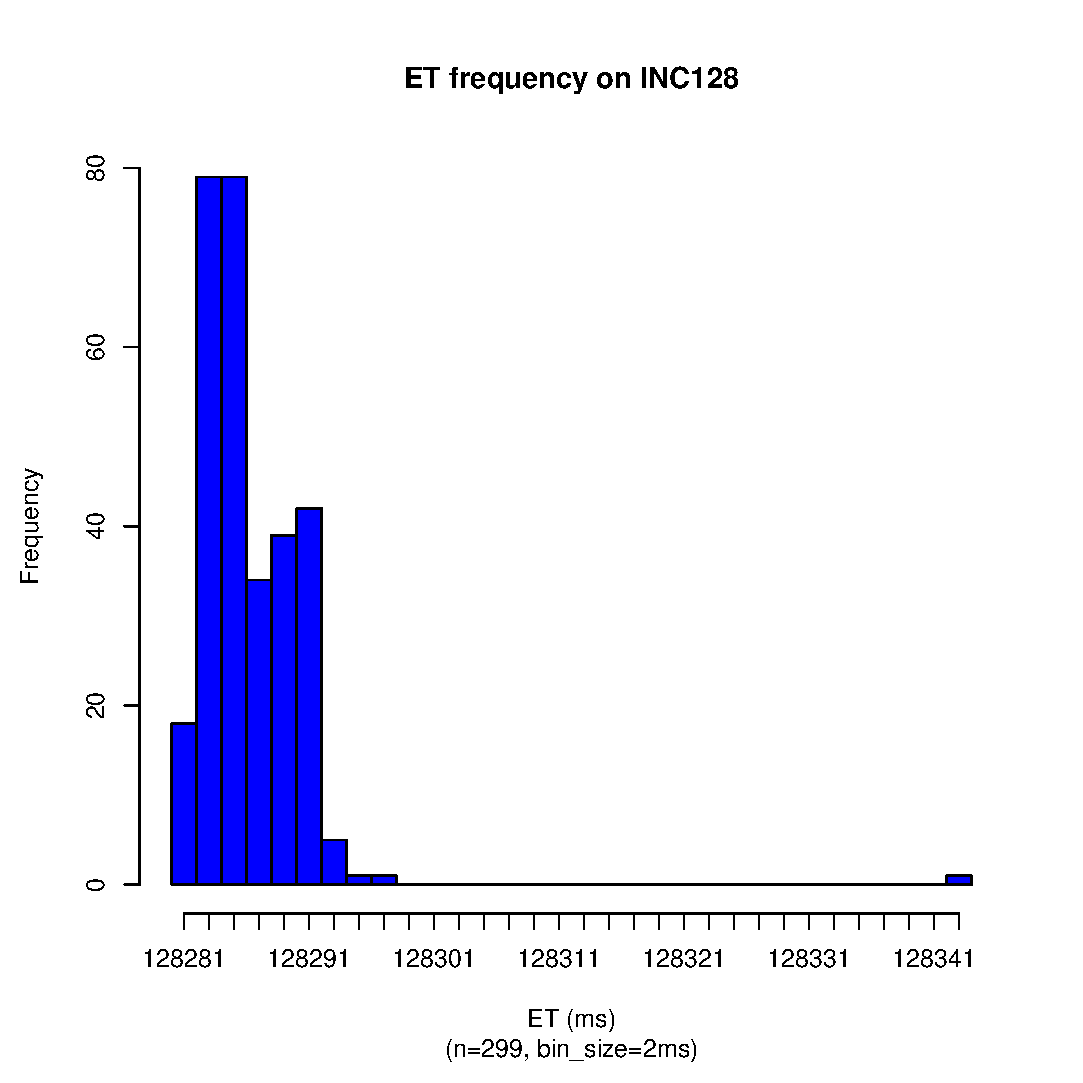
\includegraphics[scale=0.43]{repet_data1/128_sec_et_hist_v5.eps}
		\label{fig:inc128_r1_et_hist_v5}
	}
	\subfigure[ET frequency on INC256 on {\tt sodb9}]{
		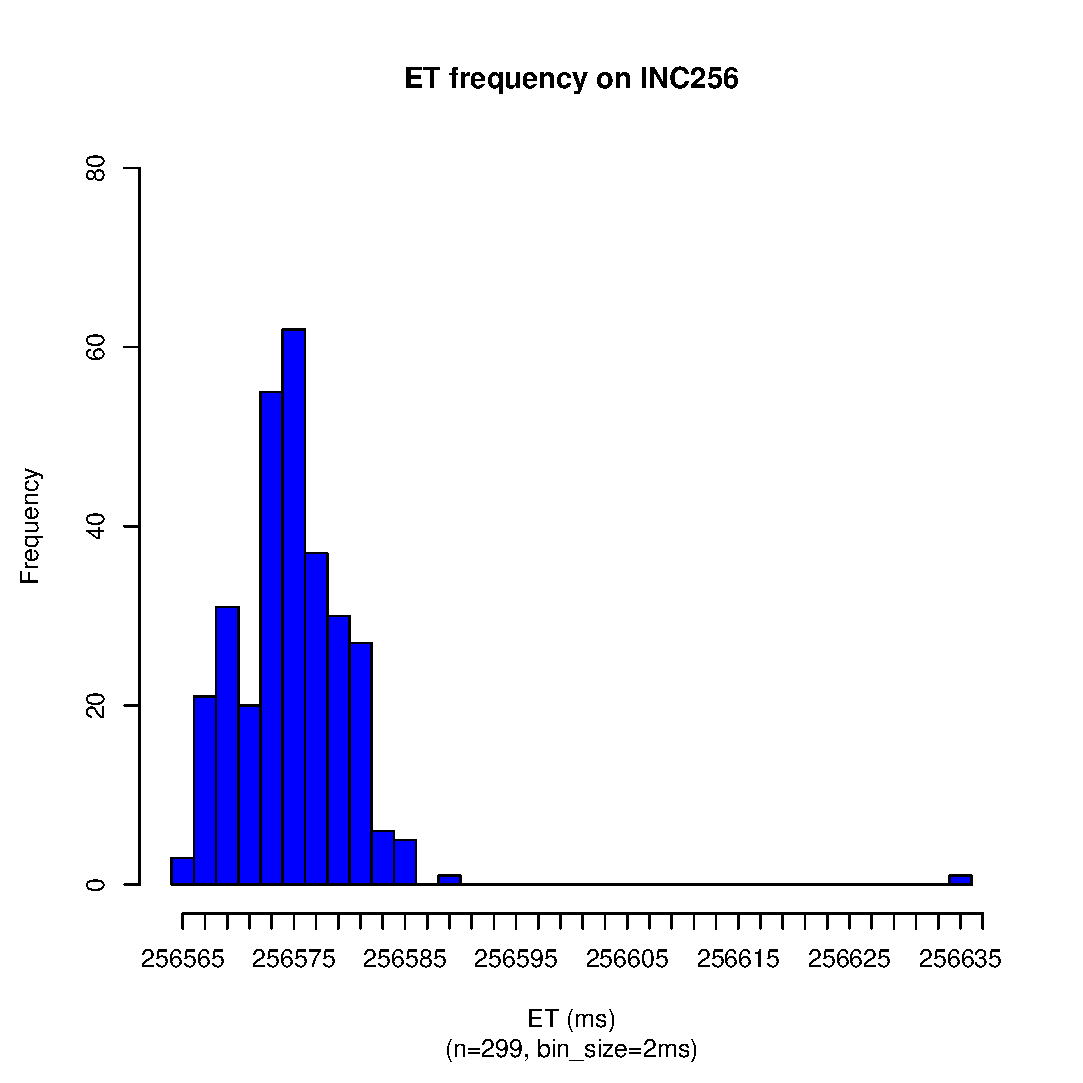
\includegraphics[scale=0.43]{repet_data1/256_sec_et_hist_v5.eps}
		\label{fig:inc256_r1_et_hist_v5}
	}
	\subfigure[ET frequency on INC512 on {\tt sodb9}]{
		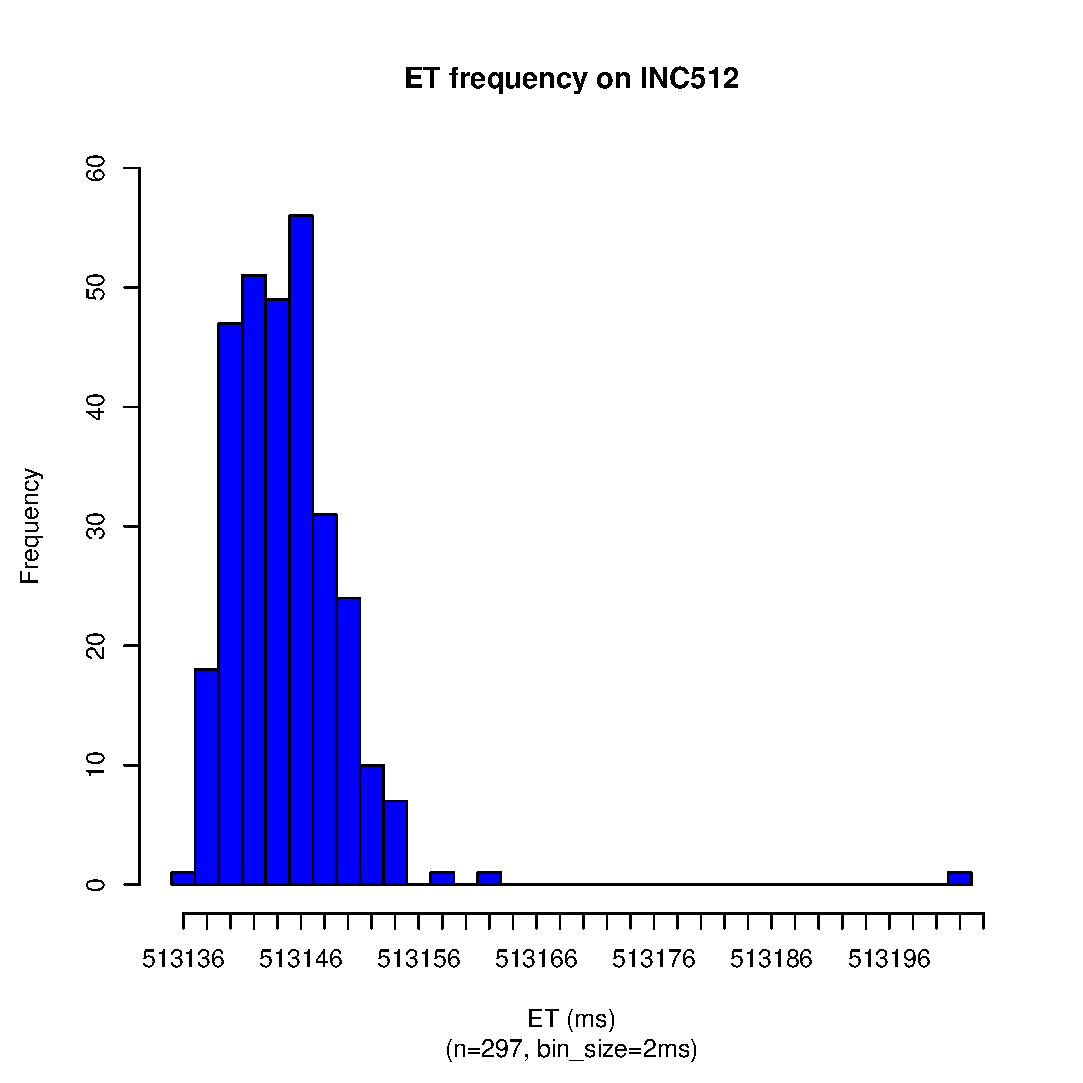
\includegraphics[scale=0.43]{repet_data1/512_sec_et_hist_v5.eps}
		\label{fig:inc512_r1_et_hist_v5}
	}
	\subfigure[ET frequency on INC1024 on {\tt sodb9}]{
		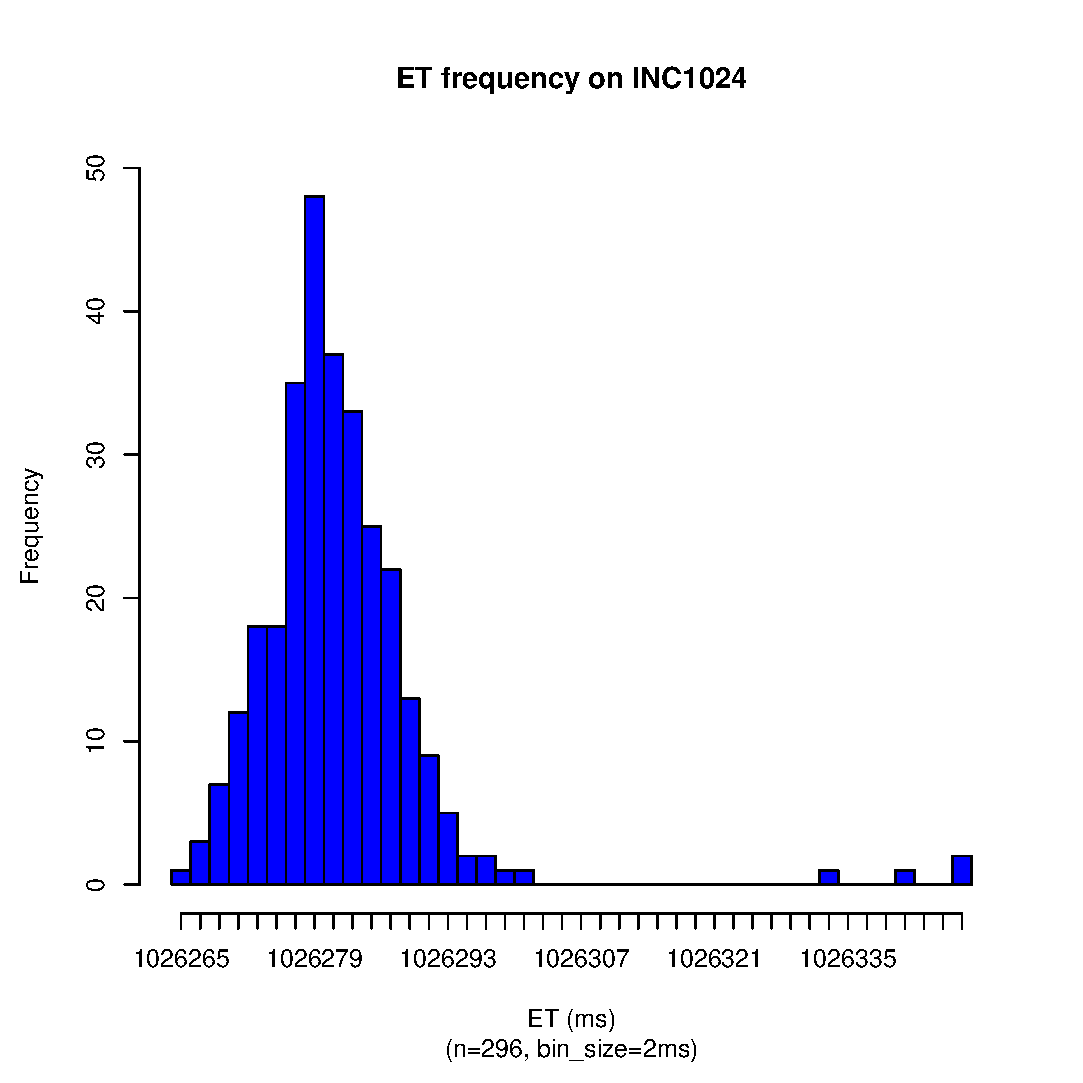
\includegraphics[scale=0.43]{repet_data1/1024_sec_et_hist_v5.eps}
		\label{fig:inc1024_r1_et_hist_v5}
	}
	\caption{ET Histograms of INC128 ... INC1024~\label{fig:s9_r1_et_hist3}}
\end{figure}

\pagebreak

\begin{figure}[t]
	\centering
	\subfigure[ET frequency on INC2048  on {\tt sodb10}]{
		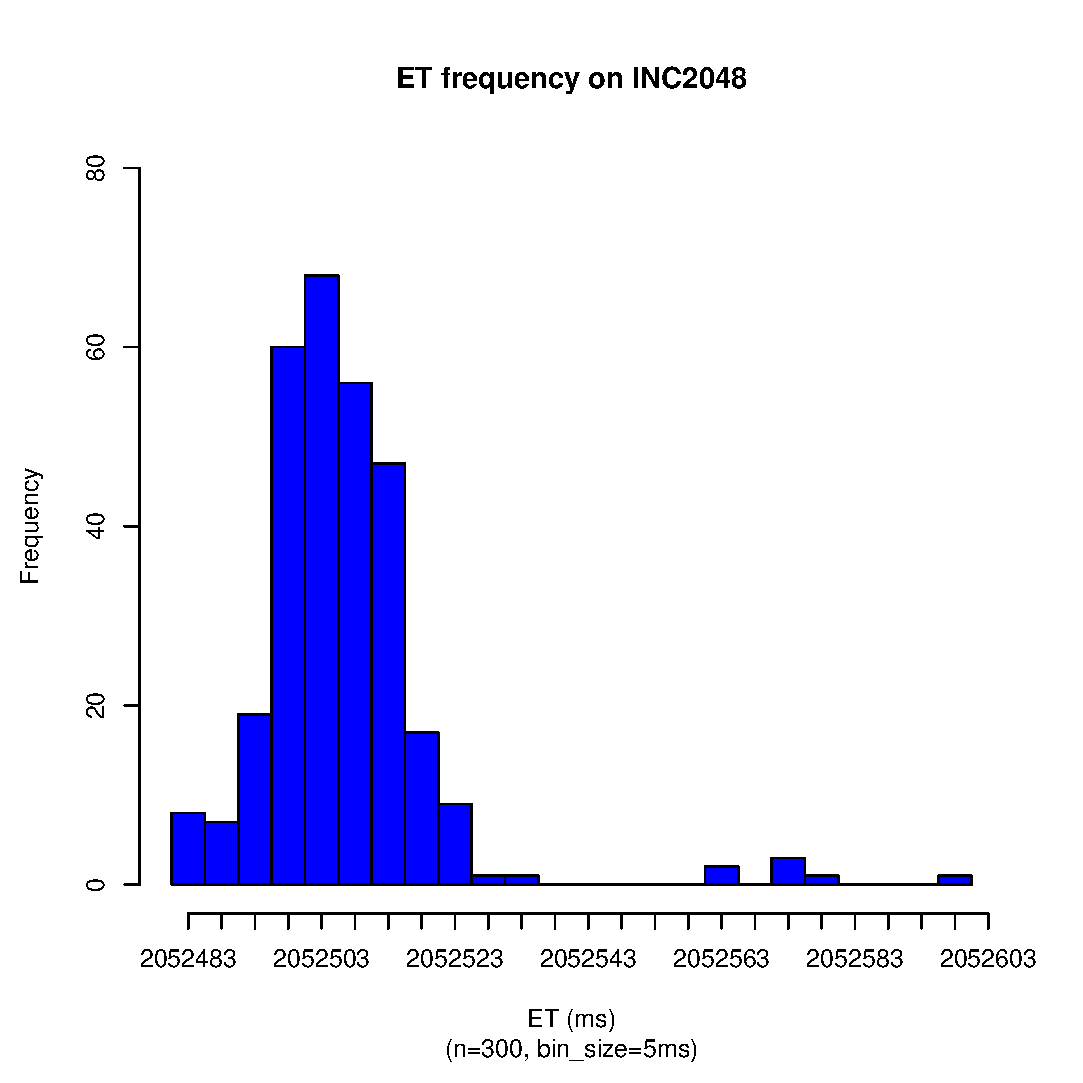
\includegraphics[scale=0.43]{repet_data1/2048_sec_et_hist_v5.eps}
		\label{fig:inc2048_r1_et_hist_v5}
	}
	\subfigure[ET frequency on INC4096 on {\tt sodb12}]{
		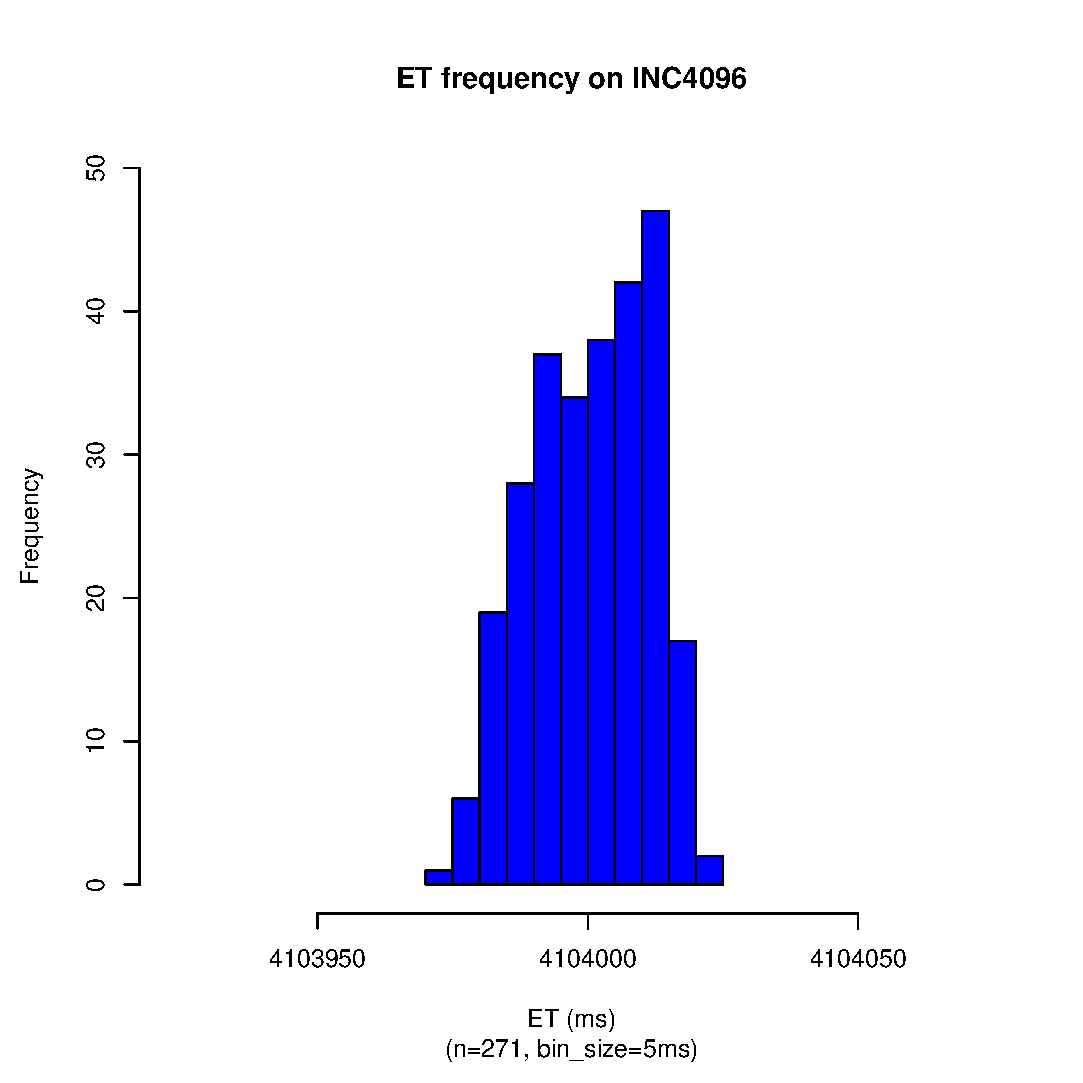
\includegraphics[scale=0.43]{repet_data1/4096_sec_et_hist_v5.eps}
		\label{fig:inc4096_r1_et_hist_v5}
	}
	\caption{ET Histograms of INC2048 and INC4096~\label{fig:s9_r1_et_hist4}}
\end{figure}

\vspace\fill
\clearpage

\subsection{PT~\label{sec:1st_pt}}

\begin{figure}[hp!]
	\centering
	\subfigure[PT frequency on INC1 on {\tt sodb9}]{
		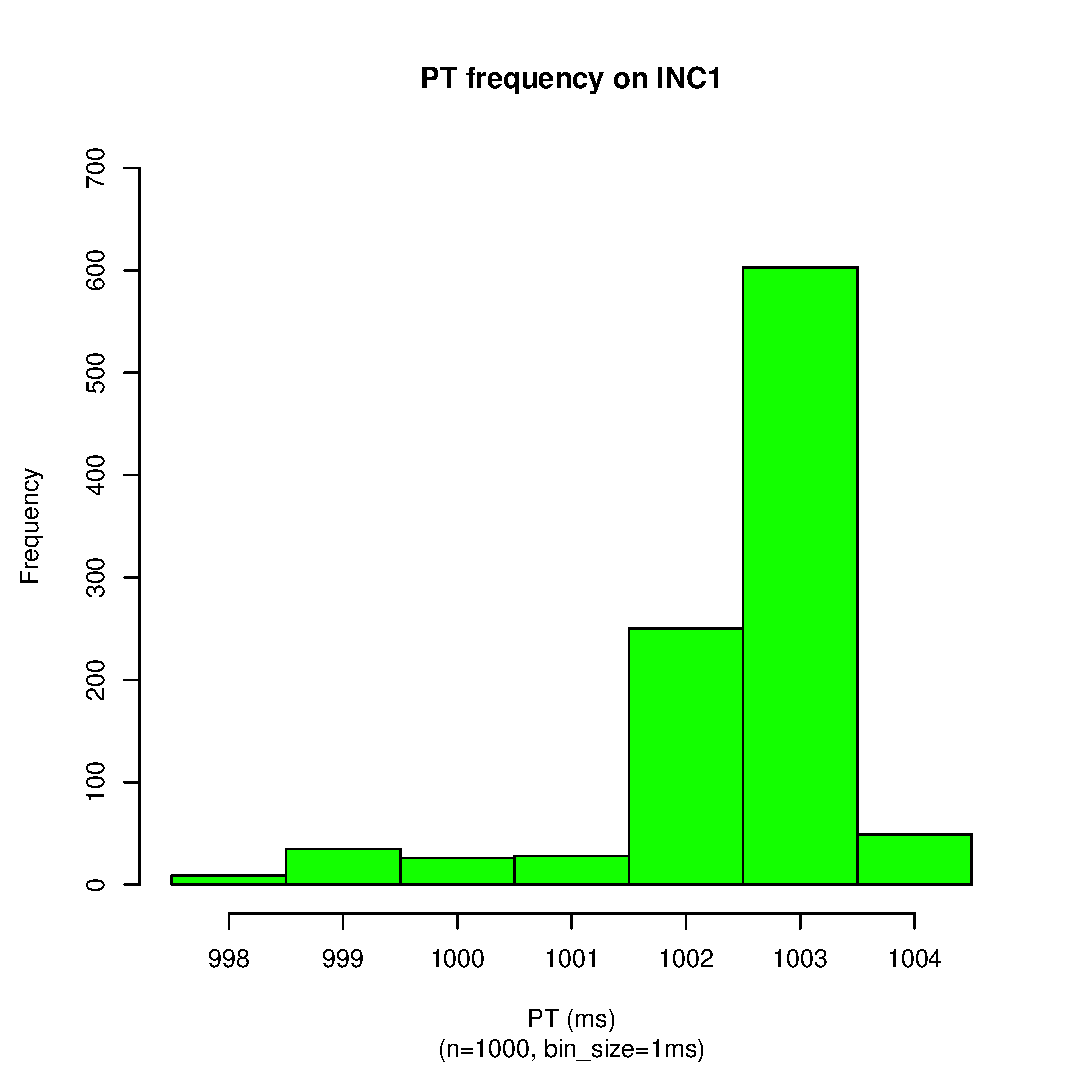
\includegraphics[scale=0.43]{repet_data1/1_sec_pt_hist_v5.eps}
		\label{fig:inc1_r1_hist_v5}
	}
	\subfigure[PT frequency on INC2 on {\tt sodb9}]{
		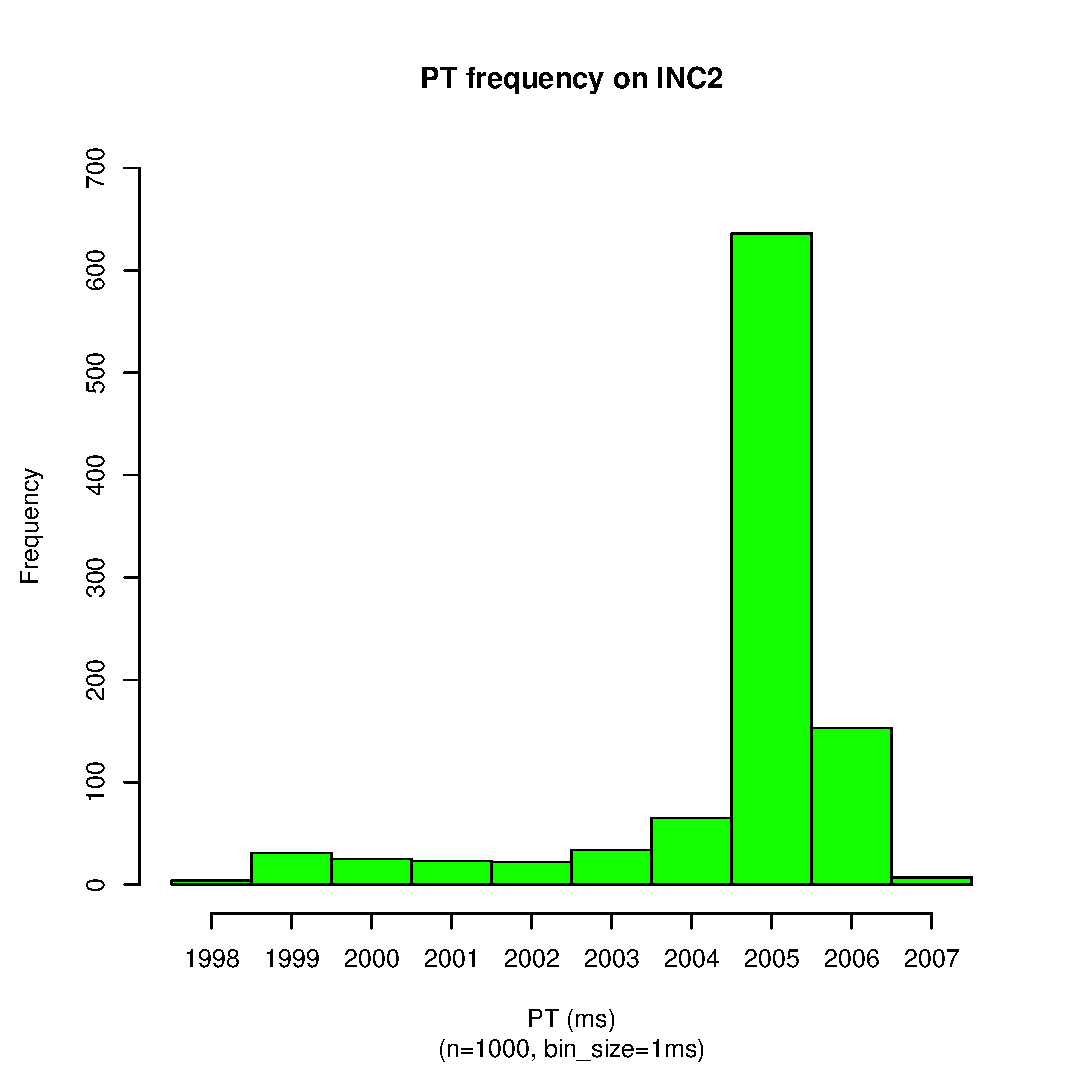
\includegraphics[scale=0.43]{repet_data1/2_sec_pt_hist_v5.eps}
		\label{fig:inc2_r1_hist_v5}
	}
	\subfigure[PT frequency on INC4 on {\tt sodb9}]{
		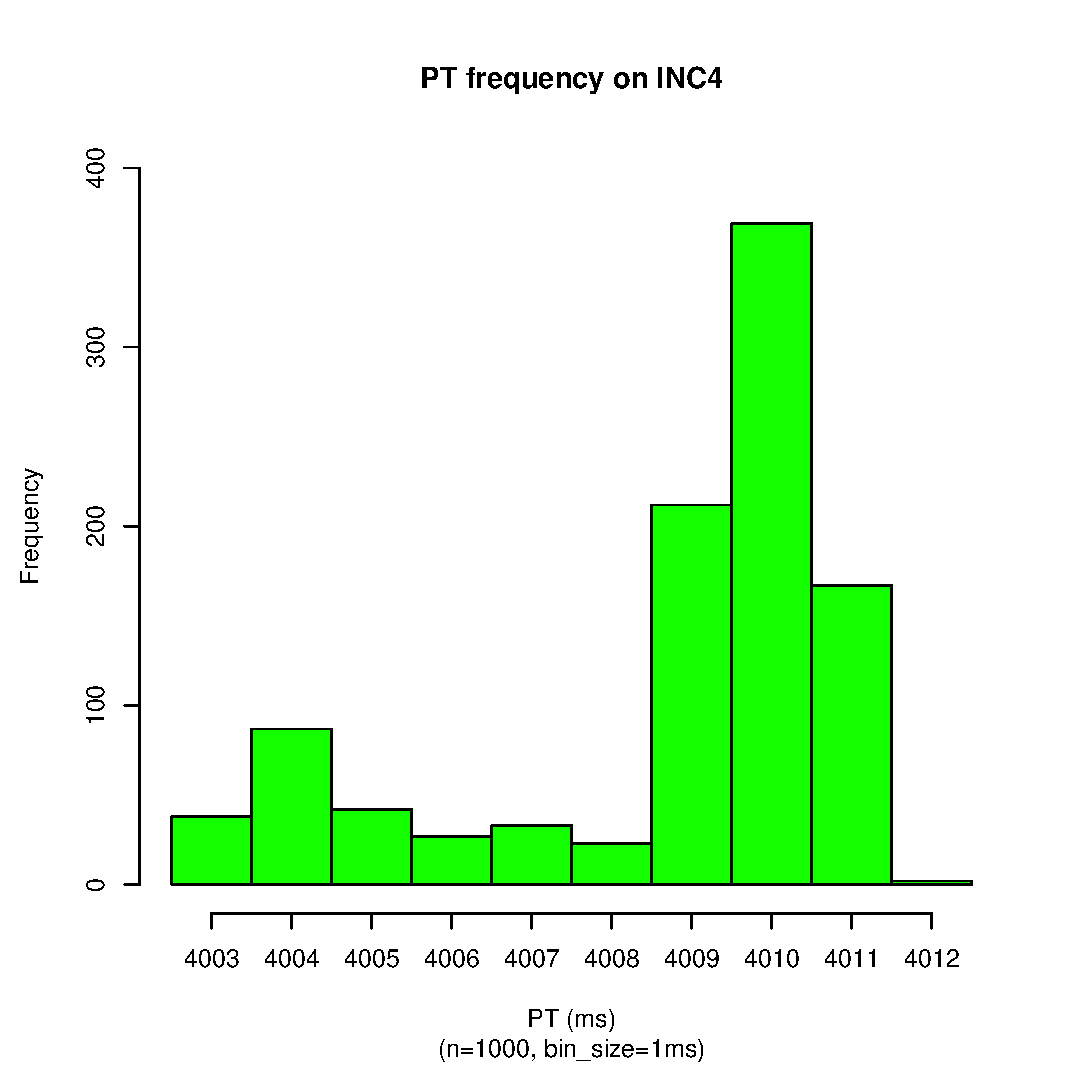
\includegraphics[scale=0.43]{repet_data1/4_sec_pt_hist_v5.eps}
		\label{fig:inc4_r1_hist_v5}
	}
	\subfigure[PT frequency on INC8 on {\tt sodb9}]{
		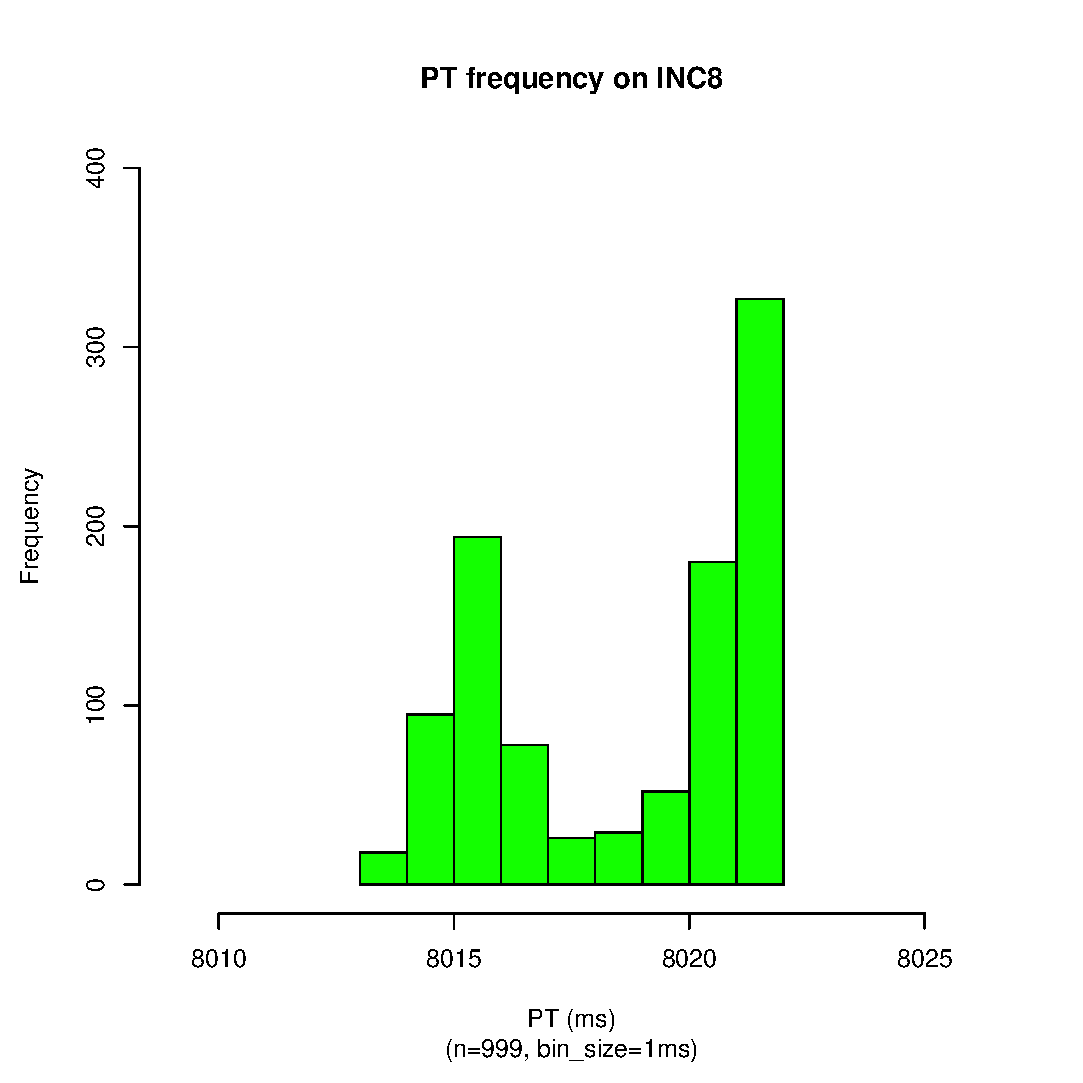
\includegraphics[scale=0.43]{repet_data1/8_sec_pt_hist_v5.eps}
		\label{fig:inc8_r1_hist_v5}
	}
	\caption{PT Histograms of INC1 ... INC8~\label{fig:s9_r1_pt_hist1}}
\end{figure}

\begin{figure}[hp!]
	\centering
	\subfigure[PT frequency on INC16 on {\tt sodb9}]{
		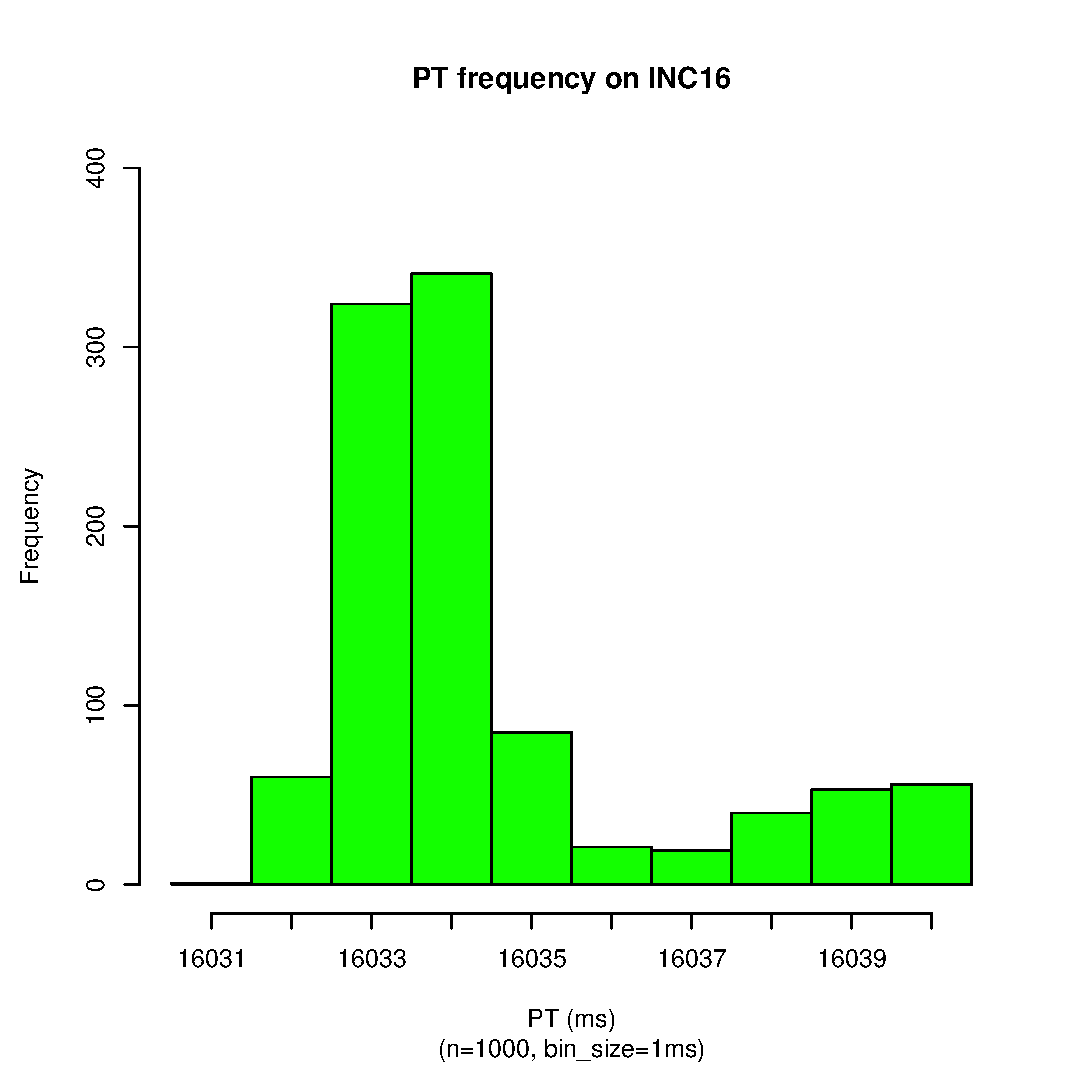
\includegraphics[scale=0.43]{repet_data1/16_sec_pt_hist_v5.eps}
		\label{fig:inc16_r1_hist_v5}
	}
	\subfigure[PT frequency on INC19 on {\tt sodb9}]{
		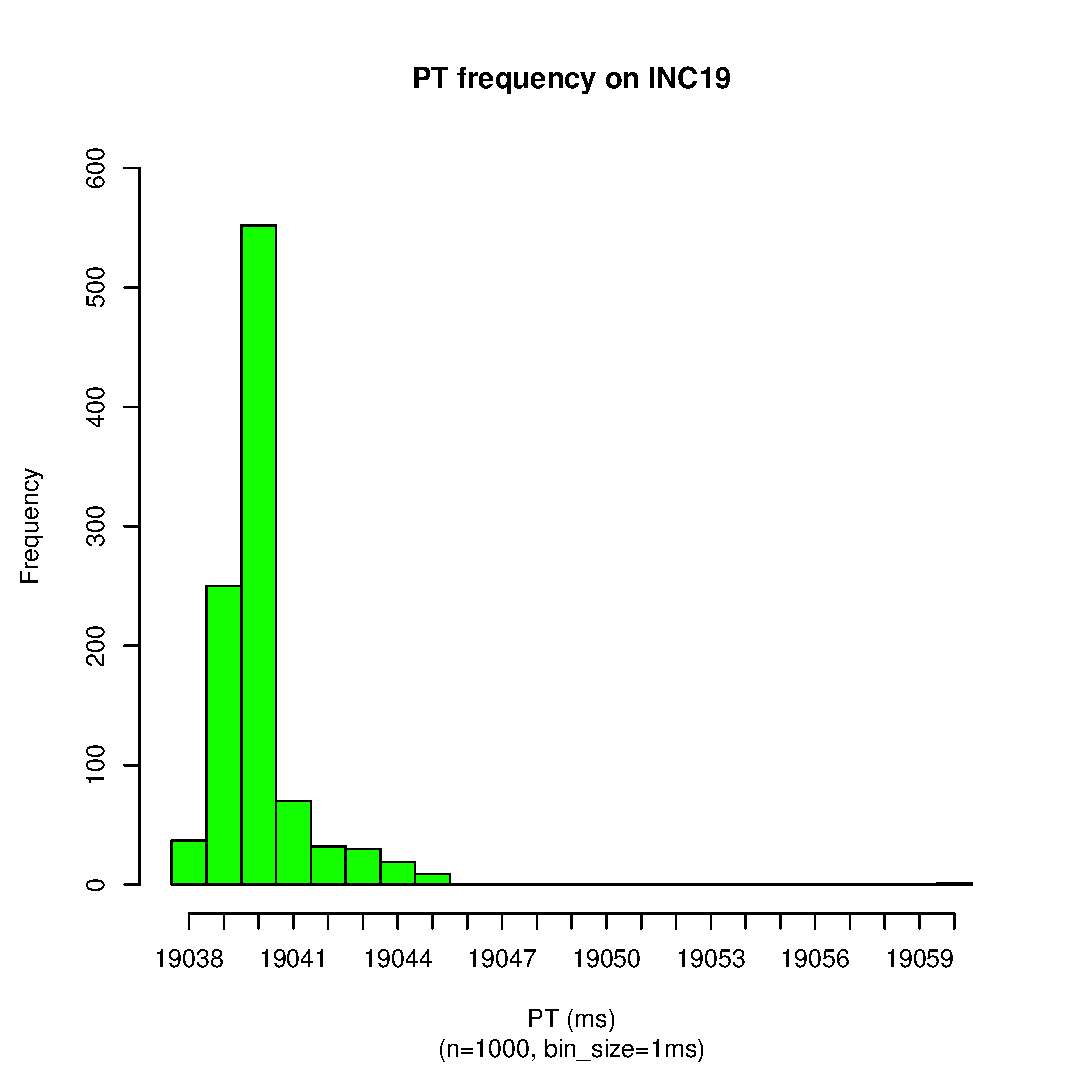
\includegraphics[scale=0.43]{repet_data1/19_sec_pt_hist.eps}
		\label{fig:inc19_hist_v4}
	}
	\subfigure[PT frequency on INC20 on {\tt sodb9}]{
		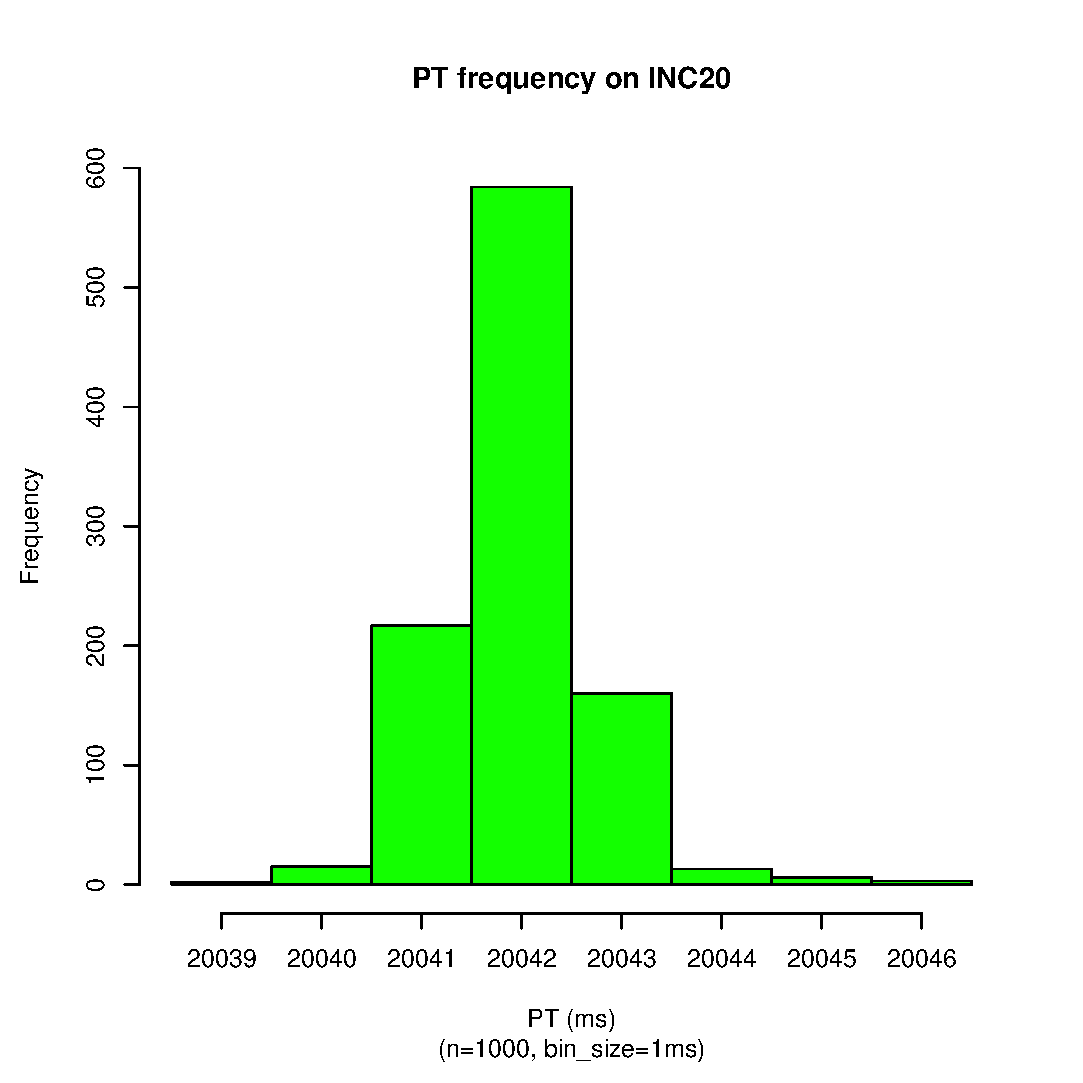
\includegraphics[scale=0.43]{repet_data1/20_sec_pt_hist.eps}
		\label{fig:inc20_hist_v4}
	}
	\subfigure[PT frequency on INC21.125 on {\tt sodb9}]{
		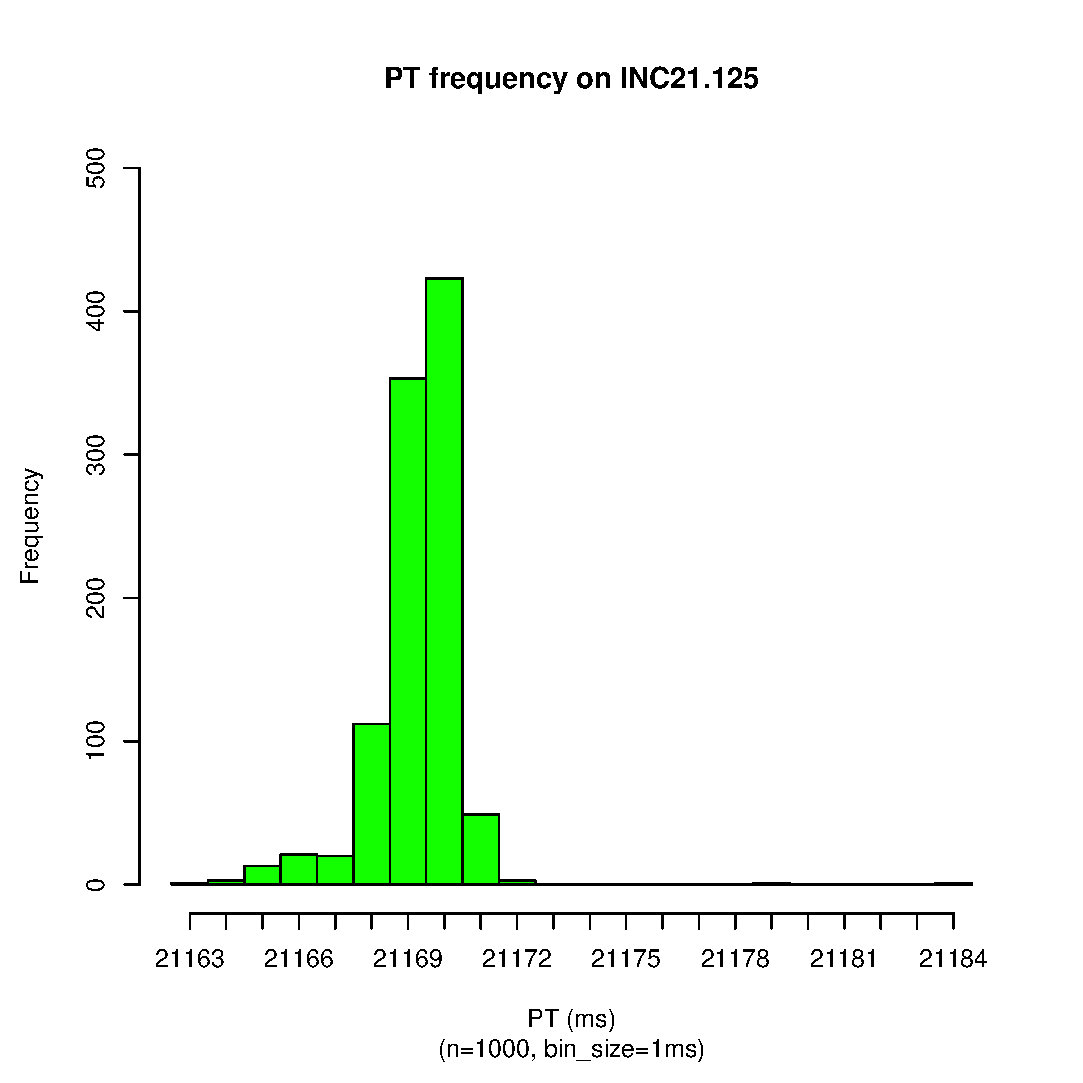
\includegraphics[scale=0.43]{repet_data1/21_125_sec_pt_hist.eps}
		\label{fig:inc21_125_hist_v4}
	}
	\caption{PT Histograms of INC16 ... INC21.125\label{fig:s9_r1_pt_hist2}}
\end{figure}

\begin{figure}[hp!]
	\centering
	\subfigure[PT frequency on INC32 on {\tt sodb9}]{
		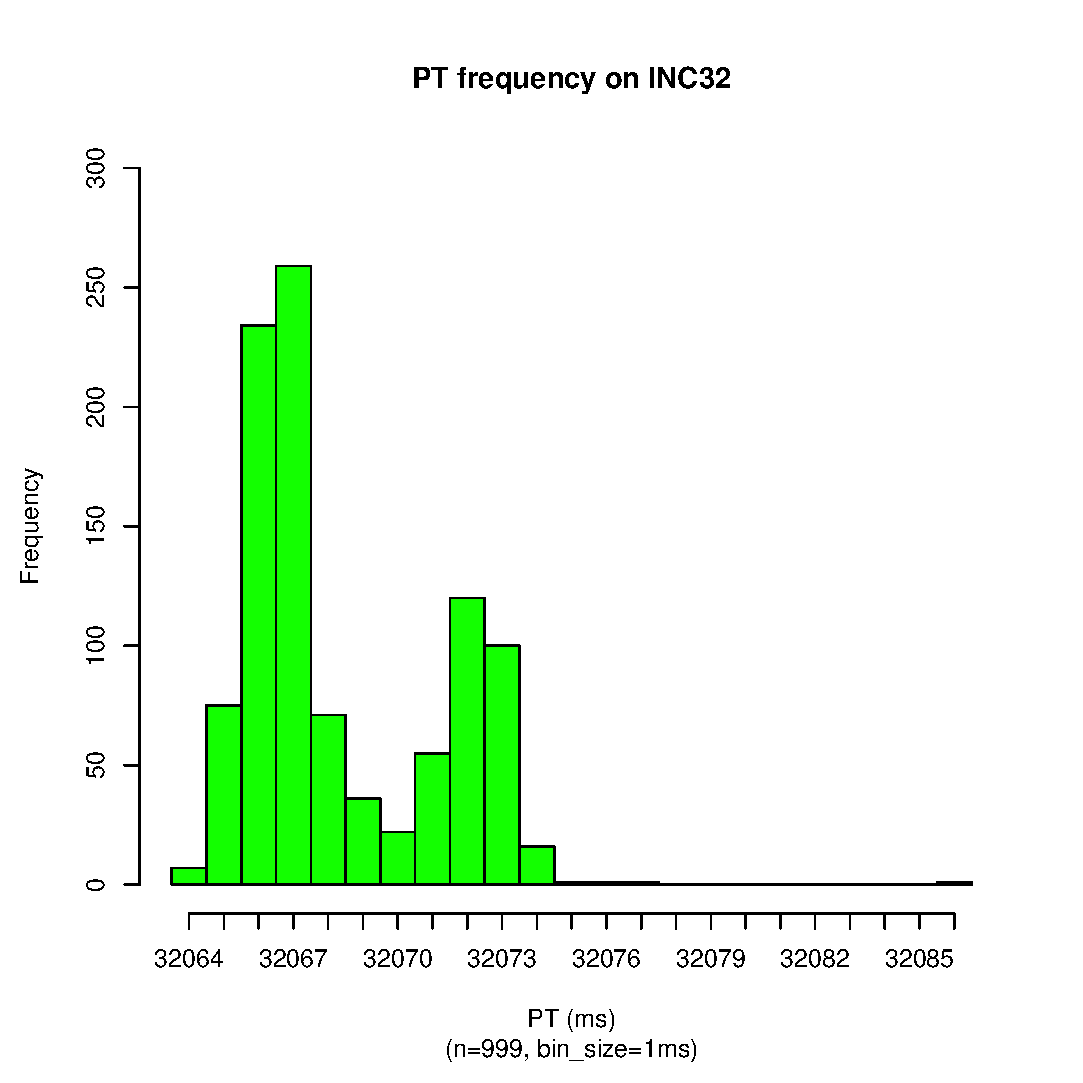
\includegraphics[scale=0.43]{repet_data1/32_sec_pt_hist_v5.eps}
		\label{fig:inc32_r1_hist_v5}
	}
	\subfigure[PT frequency on INC60 on {\tt sodb9}]{
		
\includegraphics[scale=0.43]{repet_data1/60_0_sec_pt_hist.eps}
		\label{fig:inc60_hist_v4}
	}
	\subfigure[PT frequency on INC62 on {\tt sodb9}]{
		
\includegraphics[scale=0.43]{repet_data1/62_0_sec_pt_hist.eps}
		\label{fig:inc62_hist_v4}
	}
	\subfigure[PT frequency on INC64 on {\tt sodb9}]{
		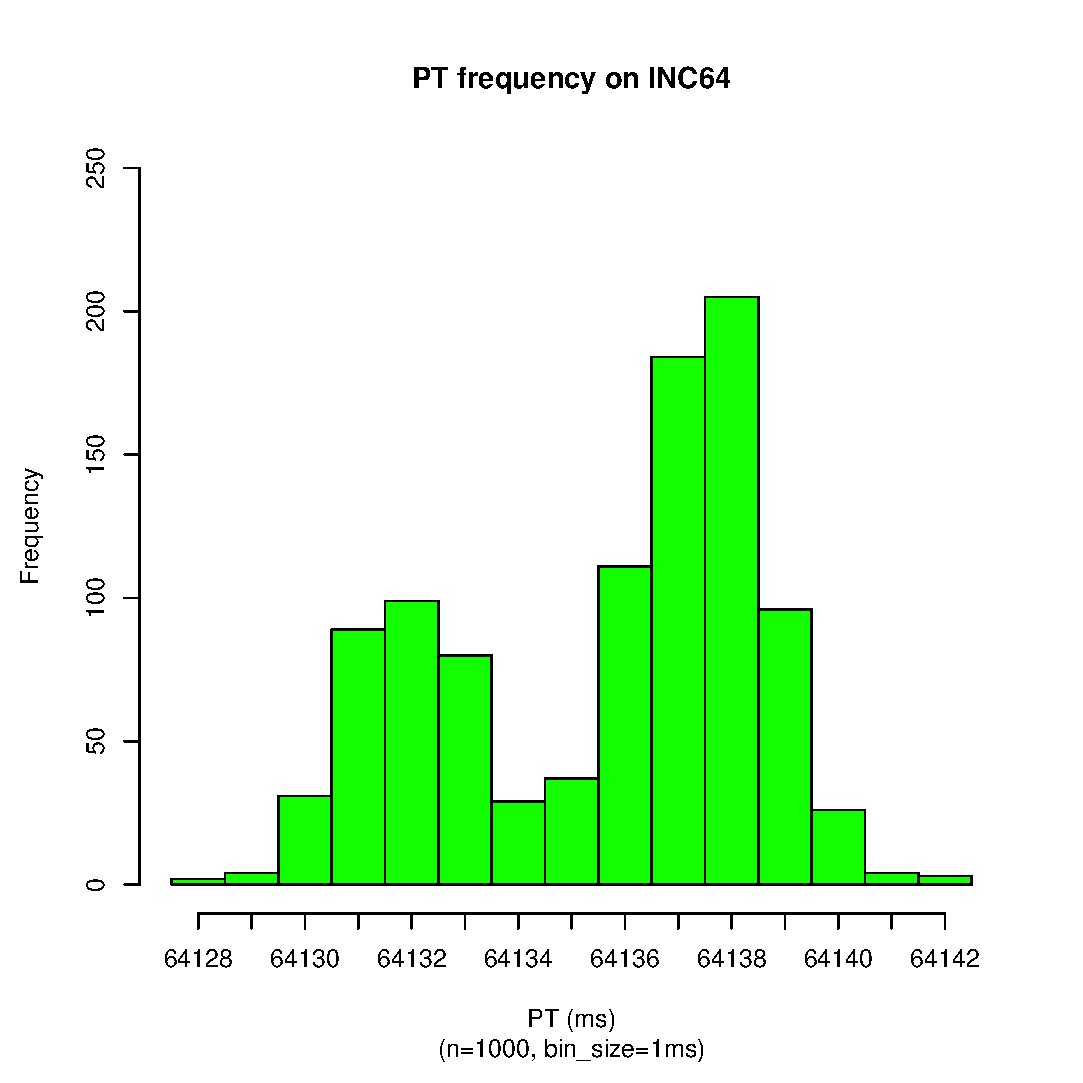
\includegraphics[scale=0.43]{repet_data1/64_sec_pt_hist_v5.eps}
		\label{fig:inc64_r1_hist_v5}
	}
	\caption{PT Histograms of INC32 ... INC64\label{fig:s9_r1_pt_hist2-2}}
\end{figure}


\begin{figure}[hp!]
	\centering
	\subfigure[PT frequency on INC128 on {\tt sodb9}]{
		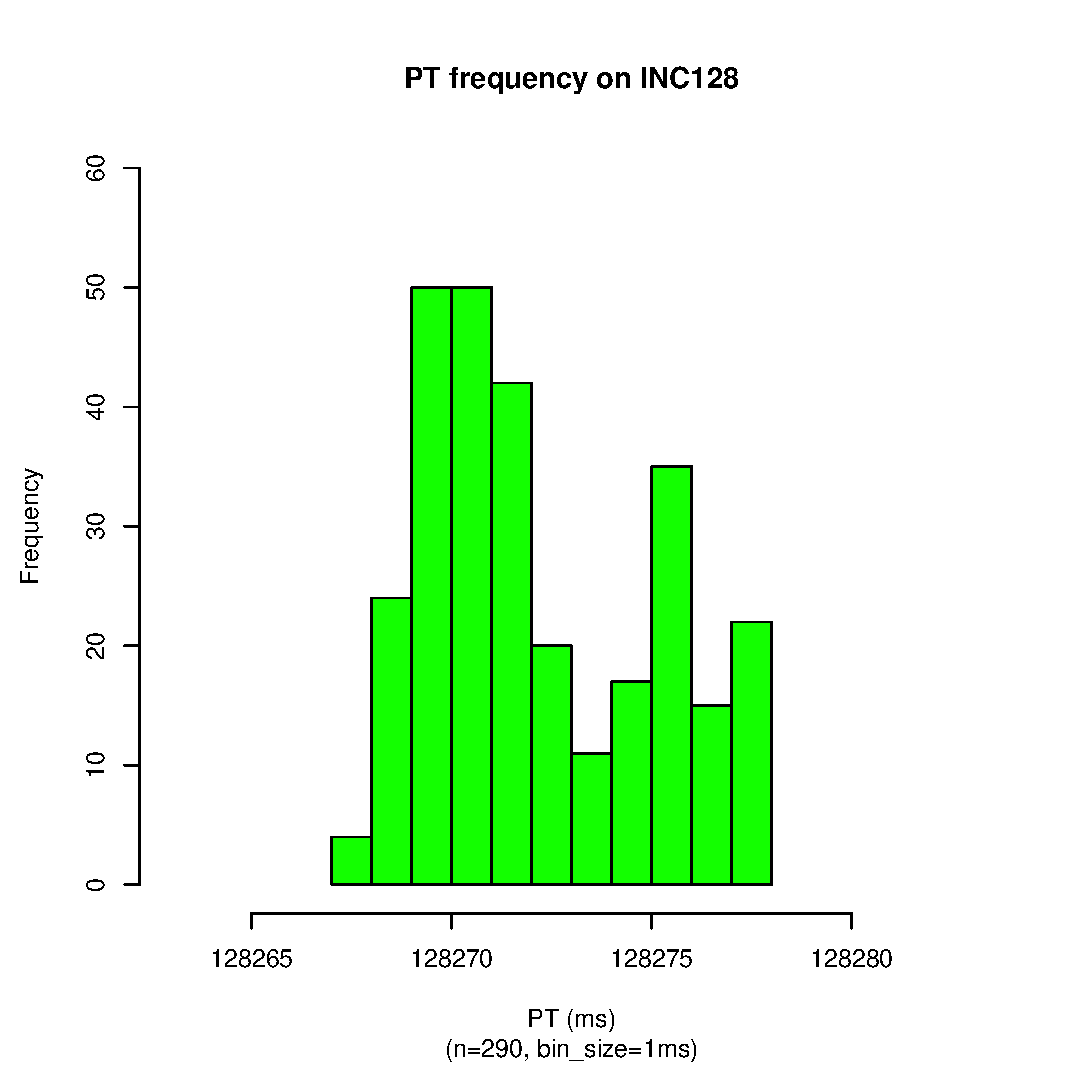
\includegraphics[scale=0.43]{repet_data1/128_sec_pt_hist_v5.eps}
		\label{fig:inc128_r1_hist_v5}
	}
	\subfigure[PT frequency on INC224 on {\tt sodb9}]{
		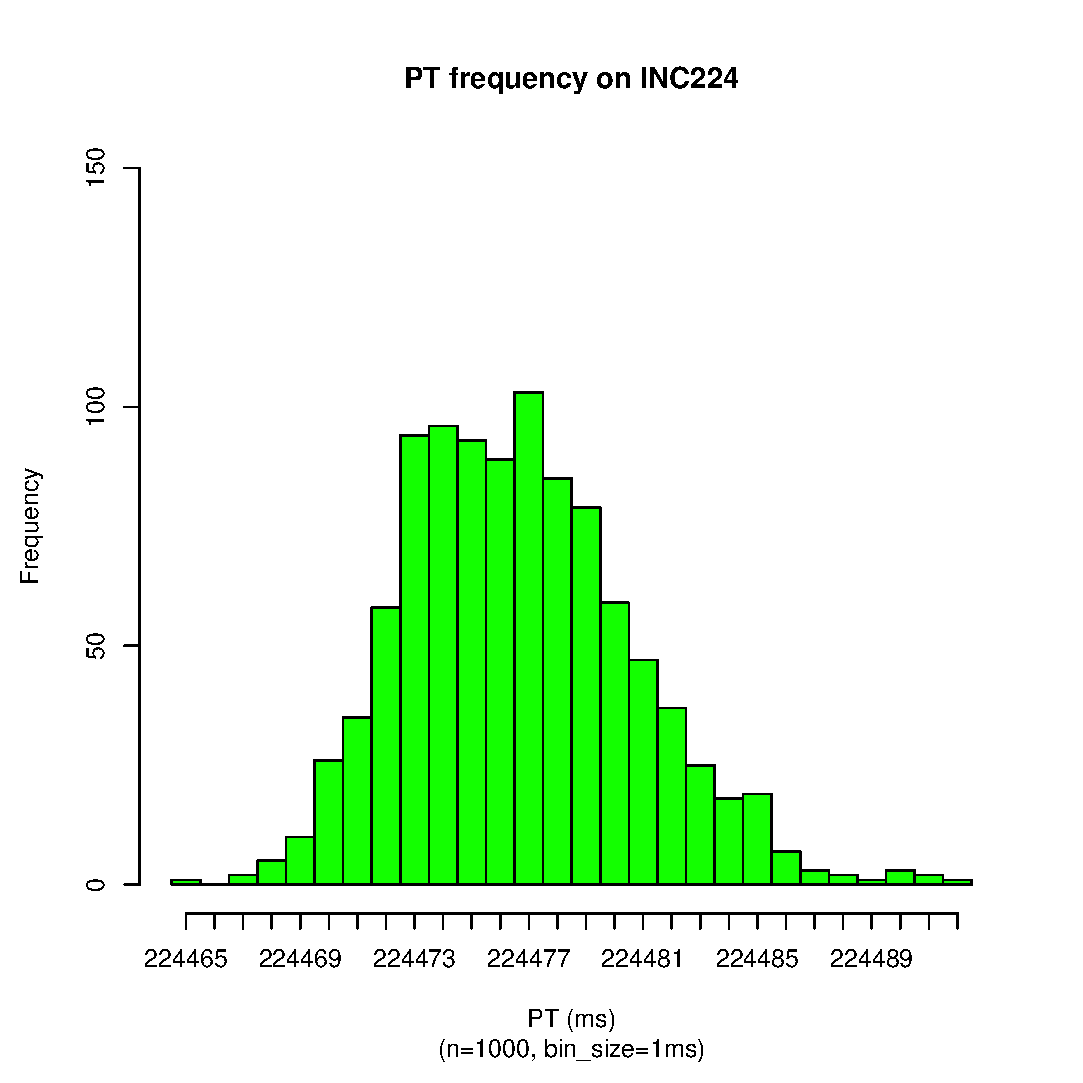
\includegraphics[scale=0.43]{repet_data1/224_sec_pt_hist.eps}
		\label{fig:inc224_v4}
	}
	\subfigure[PT frequency on INC256 on {\tt sodb9}]{
		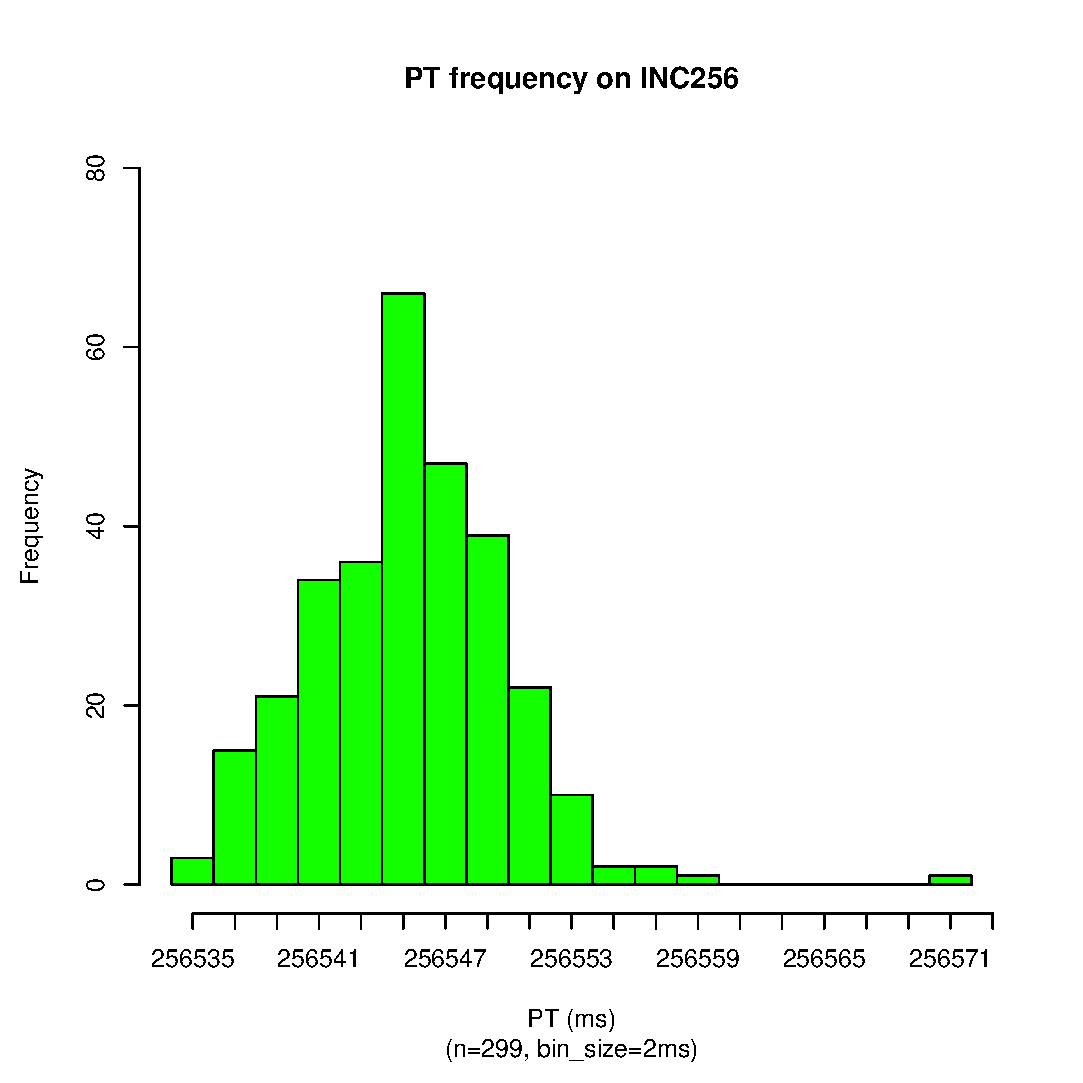
\includegraphics[scale=0.43]{repet_data1/256_sec_pt_hist_v5.eps}
		\label{fig:inc256_r1_hist_v5}
	}
	\subfigure[PT frequency on INC512 on {\tt sodb9}]{
		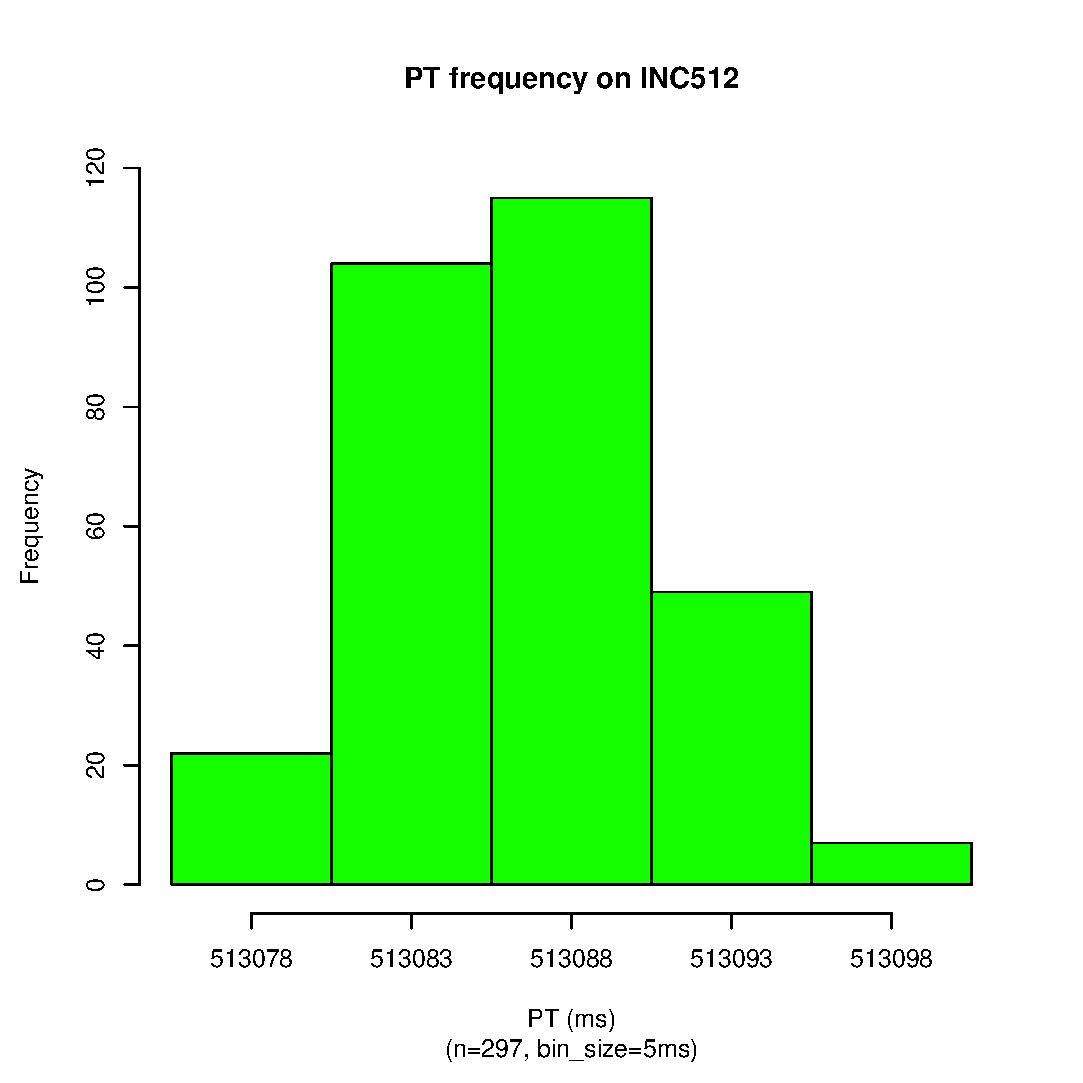
\includegraphics[scale=0.43]{repet_data1/512_sec_pt_hist_v5.eps}
		\label{fig:inc512_r1_hist_v5}
	}
	\caption{PT Histograms of INC256 ... INC1024~\label{fig:s9_r1_pt_hist3}}
\end{figure}

\begin{figure}[t]
	\centering
	\subfigure[PT frequency on INC1024 on {\tt sodb9}]{
		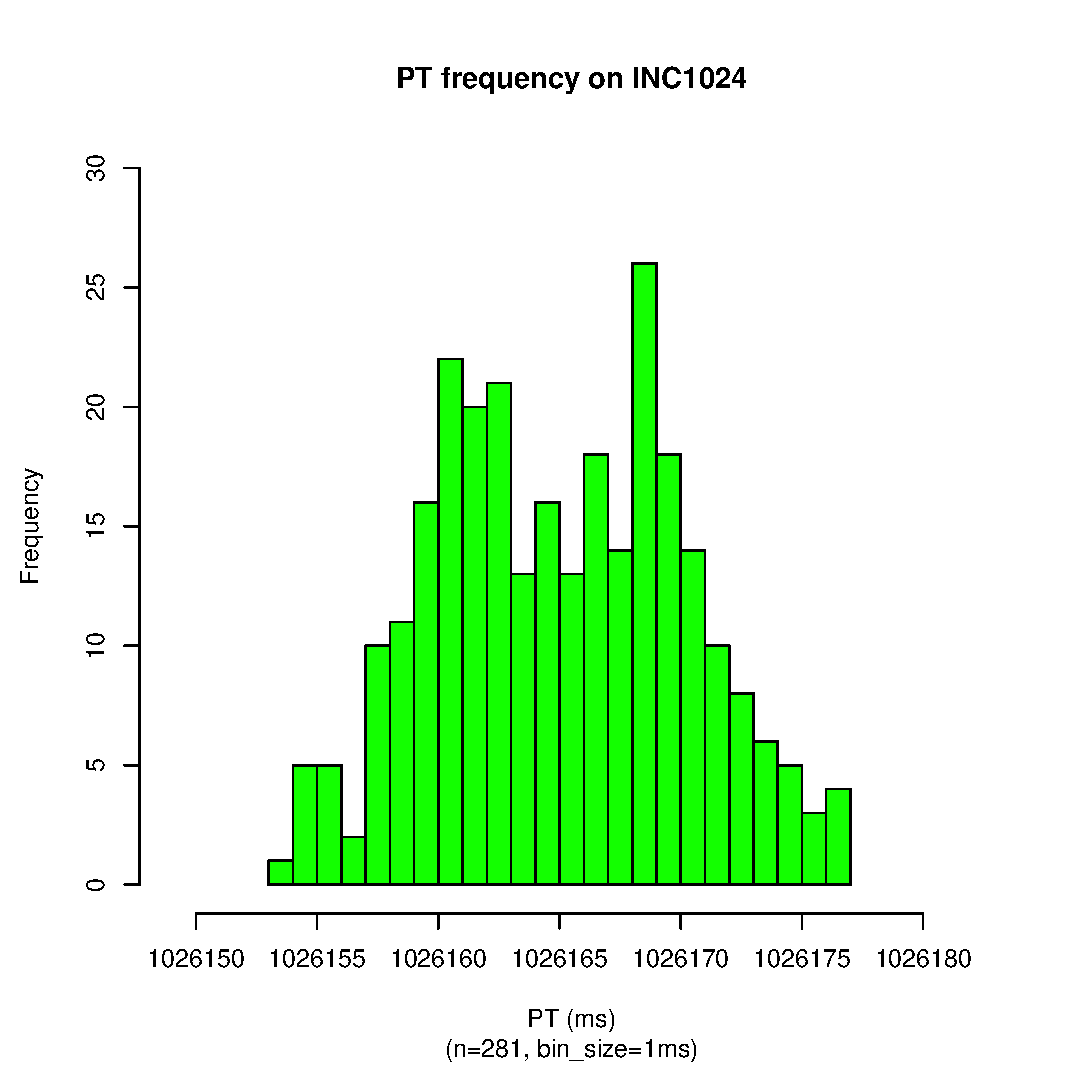
\includegraphics[scale=0.43]{repet_data1/1024_sec_pt_hist_v5.eps}
		\label{fig:inc1024_r1_hist_v5}
	}
	\subfigure[PT frequency on INC2048 on {\tt sodb10}]{
		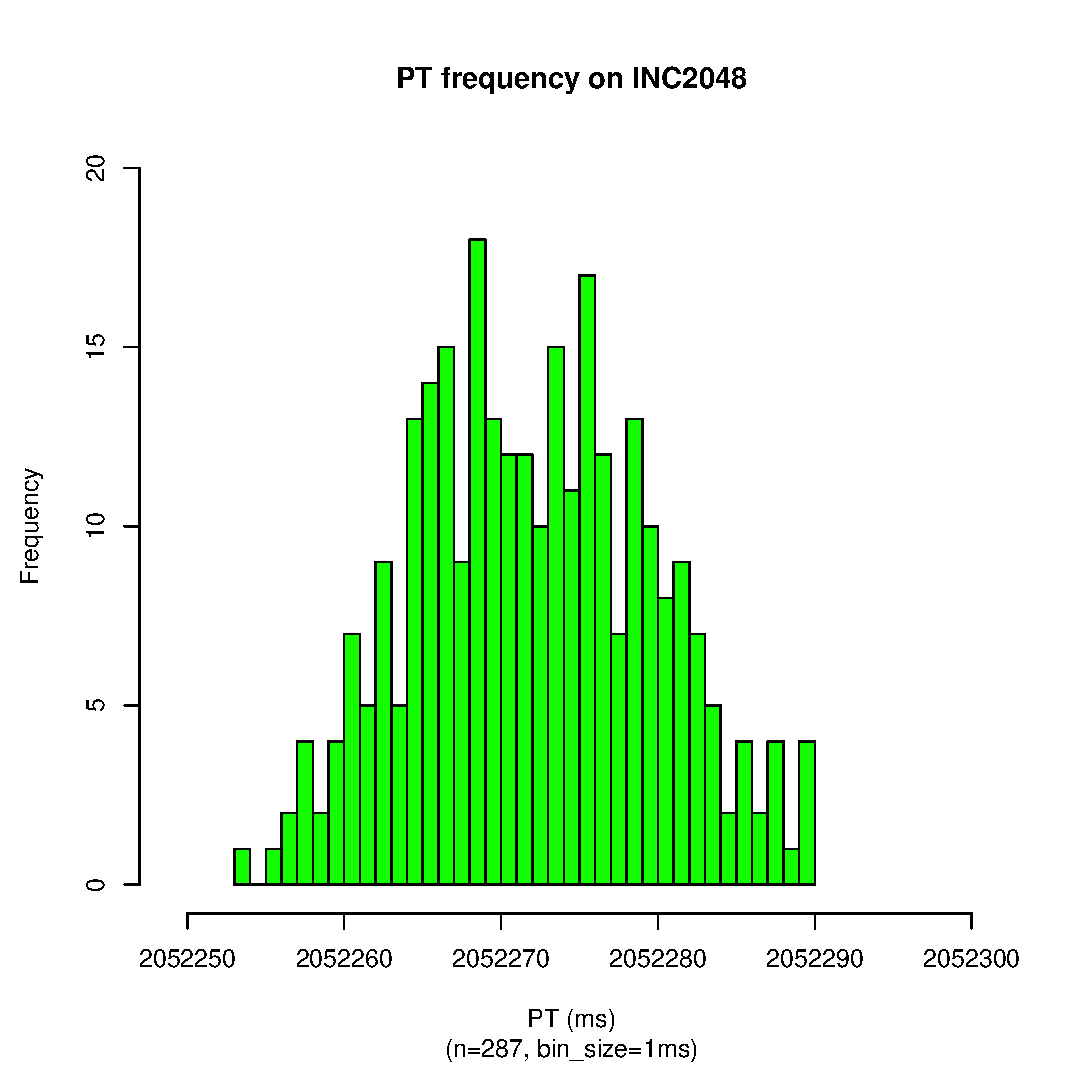
\includegraphics[scale=0.43]{repet_data1/2048_sec_pt_hist_v5.eps}
		\label{fig:inc2048_r1_hist_v5}
	}
	\subfigure[PT frequency on INC4096 on {\tt sodb12}]{
		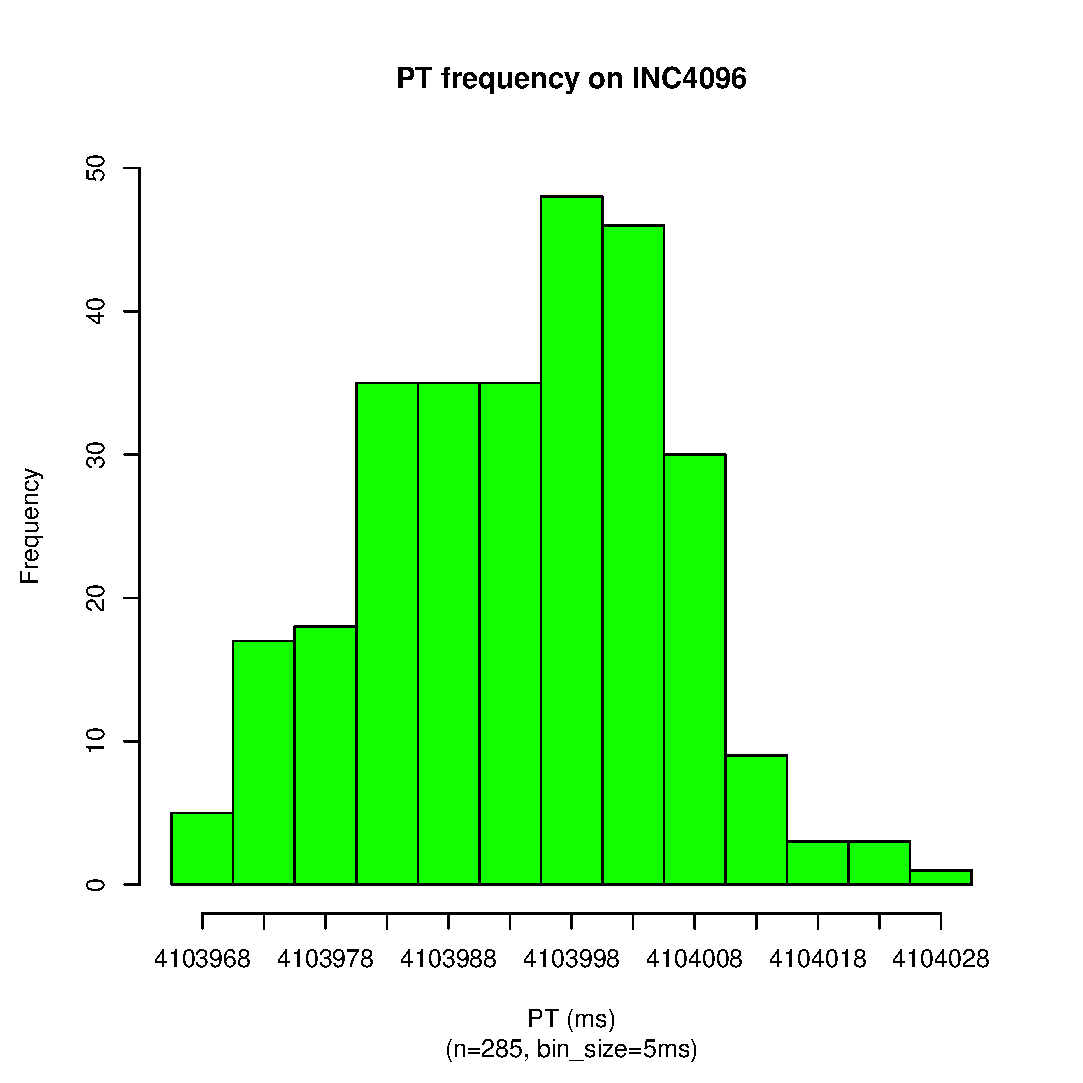
\includegraphics[scale=0.43]{repet_data1/4096_sec_pt_hist_v5.eps}
		\label{fig:inc4096_r1_hist_v5}
	}
	\caption{PT Histograms of INC1024 ... INC4096~\label{fig:s9_r1_pt_hist4}}
\end{figure}

\clearpage

\pagebreak
\newpage

\subsection{Additional Histograms}
This section exhibits the histograms of INC with some intermediate task lengths under 256 secs. 
These histograms are intended to investigate where the crossing and merge of two peaks that are consistently observed up to INC128 
happened. Table~\ref{tab:exp_notes4} provides a description of the intermediate runs. 
%and the second run of INC from 8192 seconds to 16384 seconds via EMPv5 with no Step 2.
\begin{table}[h]
\begin{center}
\begin{tabular}{|p{2cm}|p{3cm}|p{3cm}|p{4cm}|p{3.5cm}|} \hline
Machine & Task Length (sec) & Description & Experiment Period & Relevant \linebreak Histograms\\ \hline
{\tt sodb9} &  INC96$\sim$INC256 & 1000 samples, each & 2017-05-24 $\sim$ 2017-06-06 & Figs.~\ref{fig:ut_hist3}, \ref{fig:inc224_ut_hist}, and~\ref{fig:inc256_ut_hist}\\ \cline{2-4}
(plugged into {\em the upper left} power strip)	&  INC3, 6, 12, 24, 48, 72, 80, 88, 104, 112, and 120 & 1000 samples, each & 2017-06-07 $\sim$ 2017-06-16 & Figs.~\ref{fig:inc3_ut_hist}, ~\ref{fig:inc6_ut_hist}, ~\ref{fig:inc12_ut_hist}, ~\ref{fig:inc24_ut_hist},
~\ref{fig:inc48_ut_hist}, ~\ref{fig:inc72_ut_hist}, ~\ref{fig:inc80_ut_hist}, ~\ref{fig:inc88_ut_hist}, ~\ref{fig:inc104_ut_hist},~\ref{fig:inc112_ut_hist}, and~\ref{fig:inc120_ut_hist}\\ \hline
\end{tabular}
\end{center}
\vspace{-.2in}
\caption{Notes on experiment runs used for histograms\label{tab:exp_notes4}}
\end{table}

\subsubsection{ET}
Not available at this point, due to the labshelf server's unavailability for the time being.

\pagebreak

\subsubsection{PT}
%The histograms of INC1 through INC4096 are 
%the same as those of Figures~\ref{fig:s9_r1_pt_hist1},~\ref{fig:s9_r1_pt_hist2},~\ref{fig:s9_r1_pt_hist3}, and~\ref{fig:s9_r1_pt_hist4}. 

\begin{figure}[hp!]
	\centering
	\subfigure[PT frequency on INC3  on {\tt sodb9}]{
		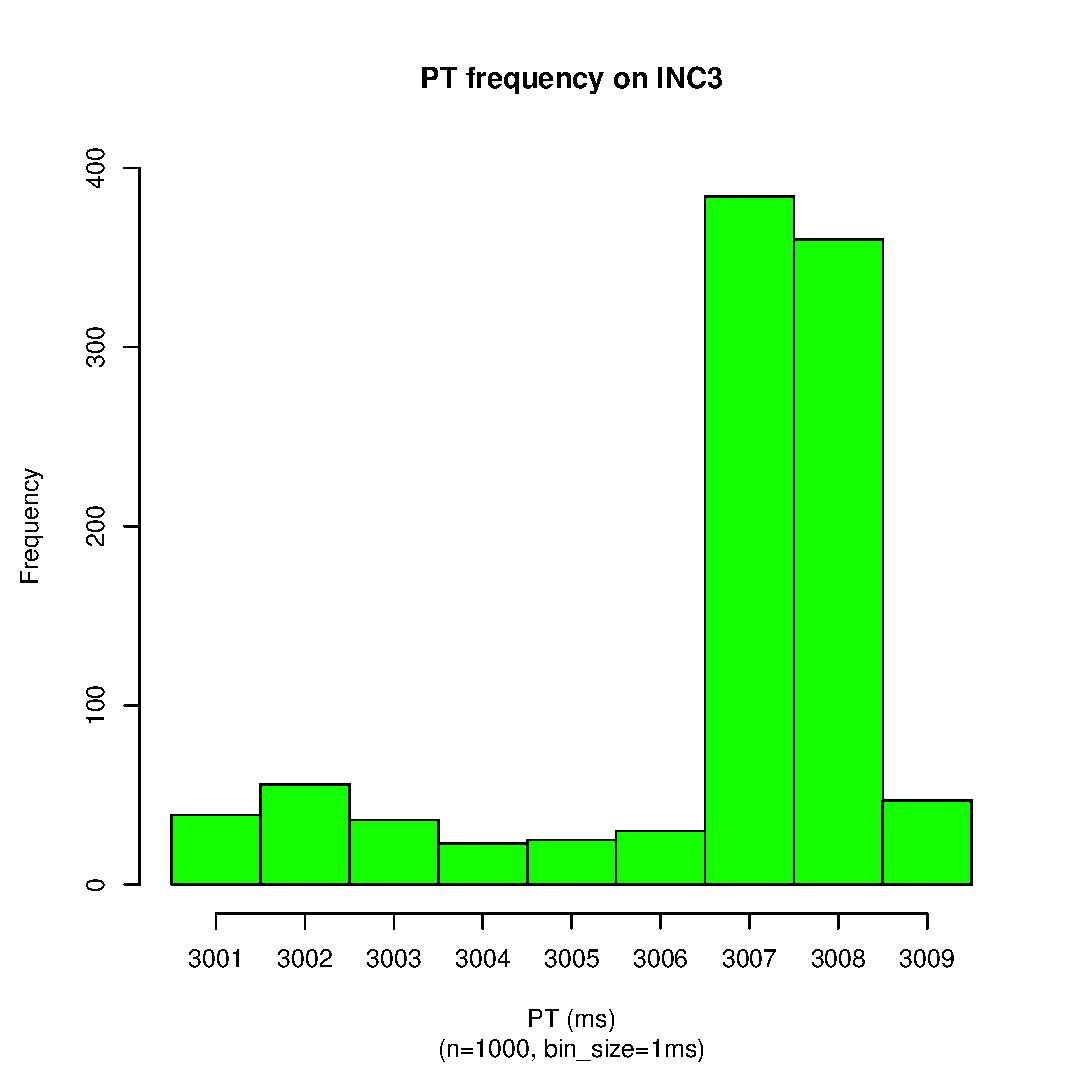
\includegraphics[scale=0.43]{u_s_time/3_sec_pt_hist.eps}
		\label{fig:inc3_pt_hist}
	}
	\subfigure[PT frequency on INC6 on {\tt sodb9}]{
		\includegraphics[scale=0.43]{u_s_time/6_sec_pt_hist.eps}
		\label{fig:inc6_pt_hist}
	}
	\subfigure[PT frequency on INC12  on {\tt sodb9}]{
		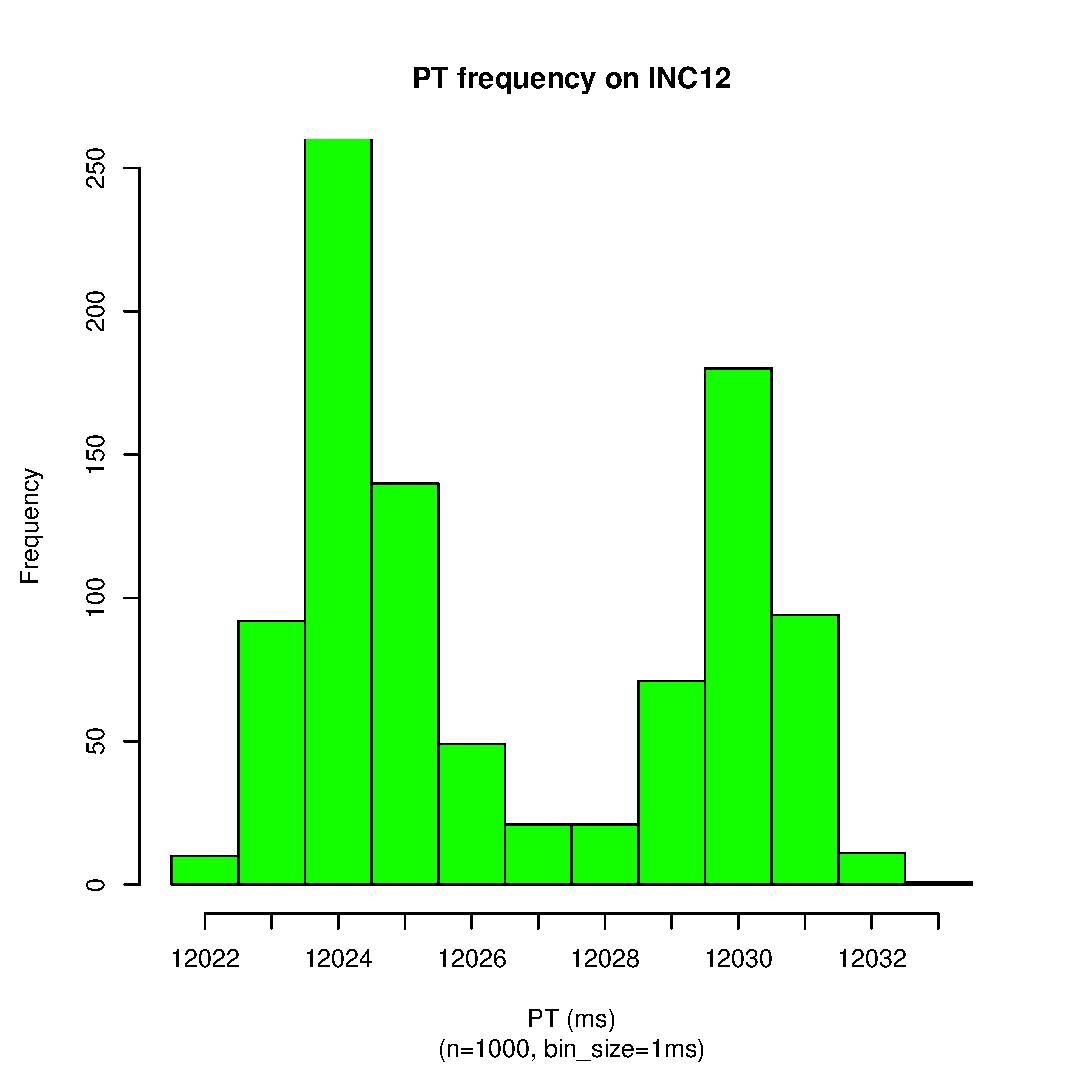
\includegraphics[scale=0.43]{u_s_time/12_sec_pt_hist.eps}
		\label{fig:inc12_pt_hist}
	}
	\subfigure[PT frequency on INC24 on {\tt sodb9}]{
		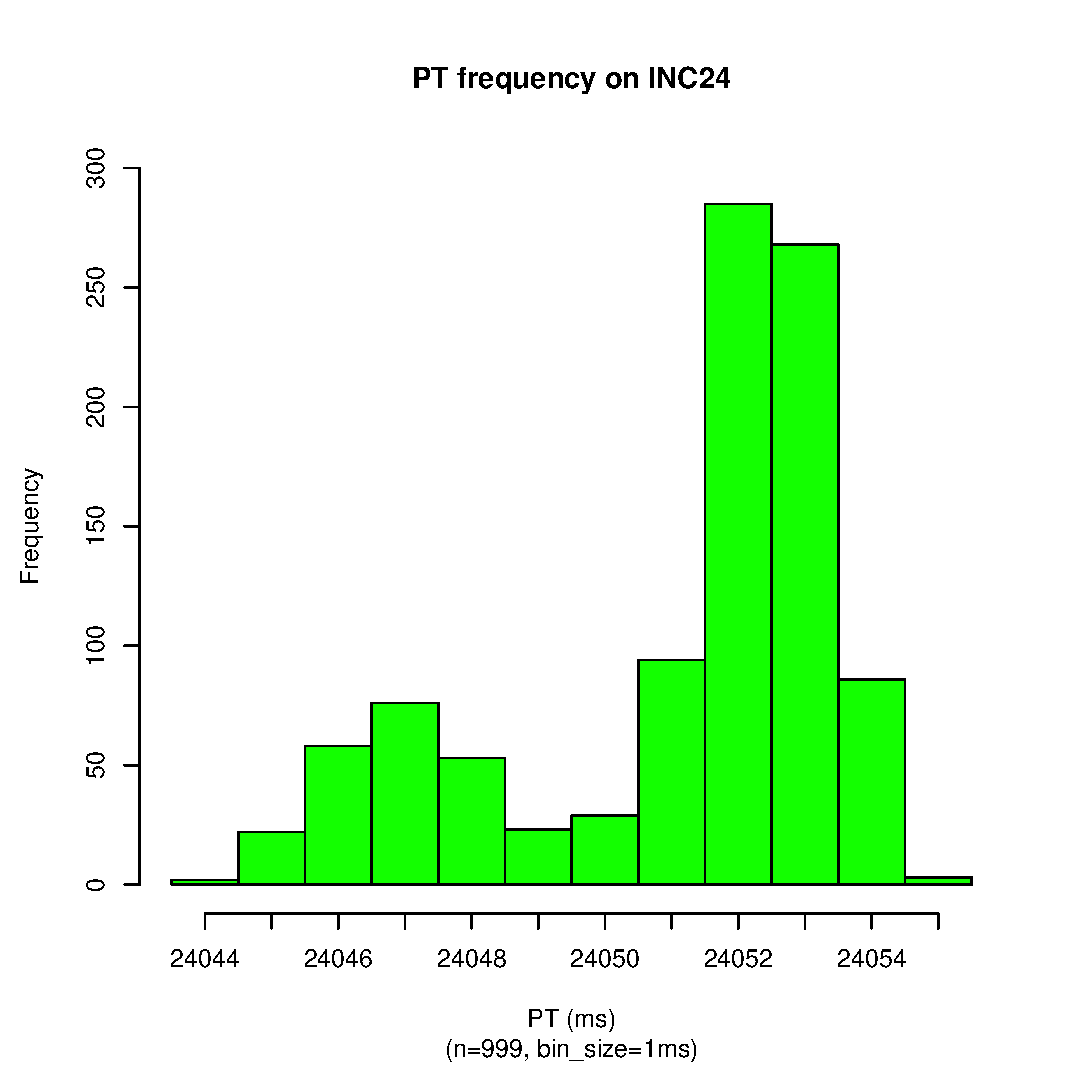
\includegraphics[scale=0.43]{u_s_time/24_sec_pt_hist.eps}
		\label{fig:inc24_pt_hist}
	}
	\caption{PT Histograms of INC3 ... INC24~\label{fig:new_pt_hist1}}
\end{figure}

\pagebreak
\newpage

\begin{figure}[hp!]
	\centering
	\subfigure[PT frequency on INC48 on {\tt sodb9}]{
		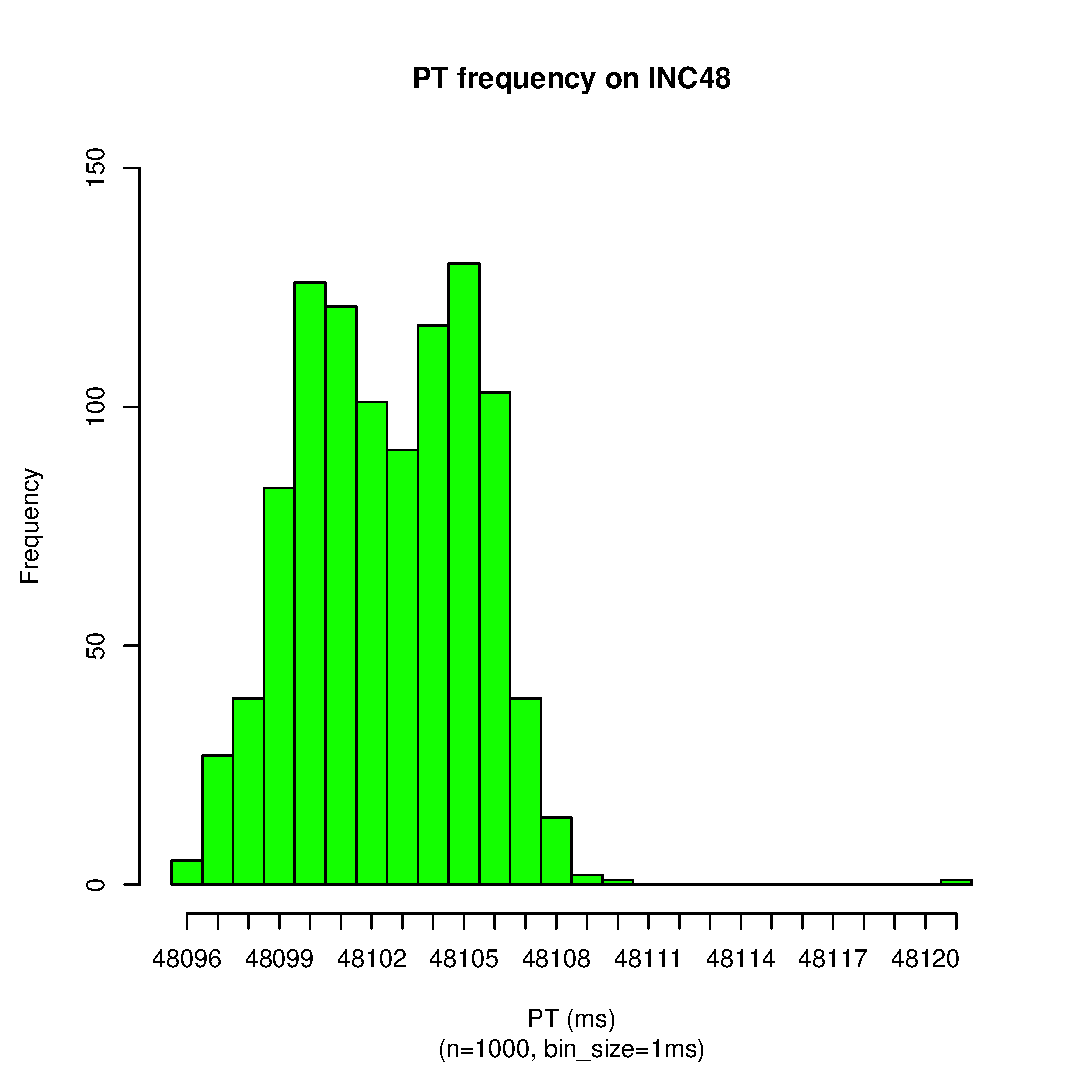
\includegraphics[scale=0.43]{u_s_time/48_sec_pt_hist.eps}
		\label{fig:inc48_pt_hist}
	}
	\subfigure[PT frequency on INC72 on {\tt sodb9}]{
		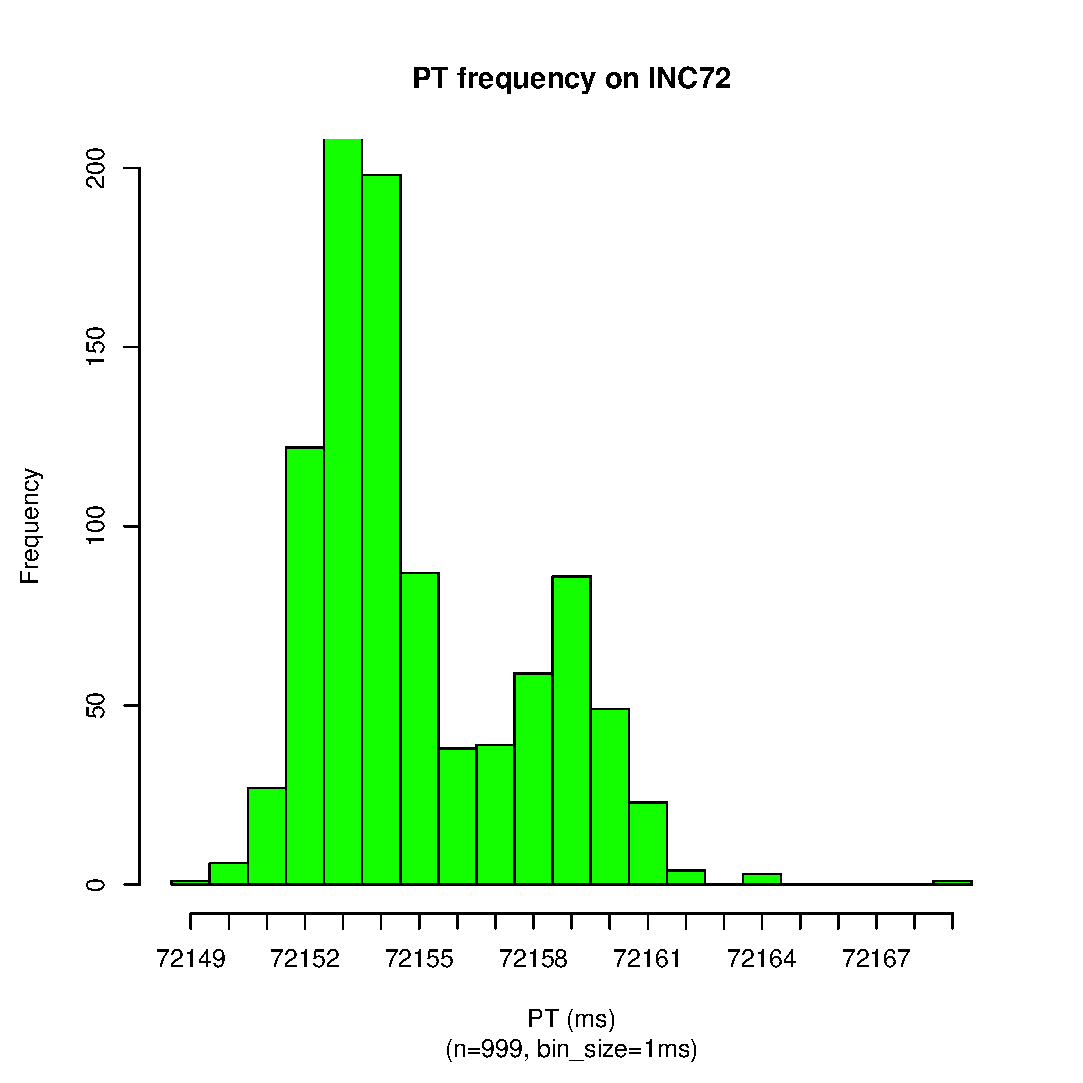
\includegraphics[scale=0.43]{u_s_time/72_sec_pt_hist.eps}
		\label{fig:inc72_pt_hist}
	}
	\subfigure[PT frequency on INC80 on {\tt sodb9}]{
		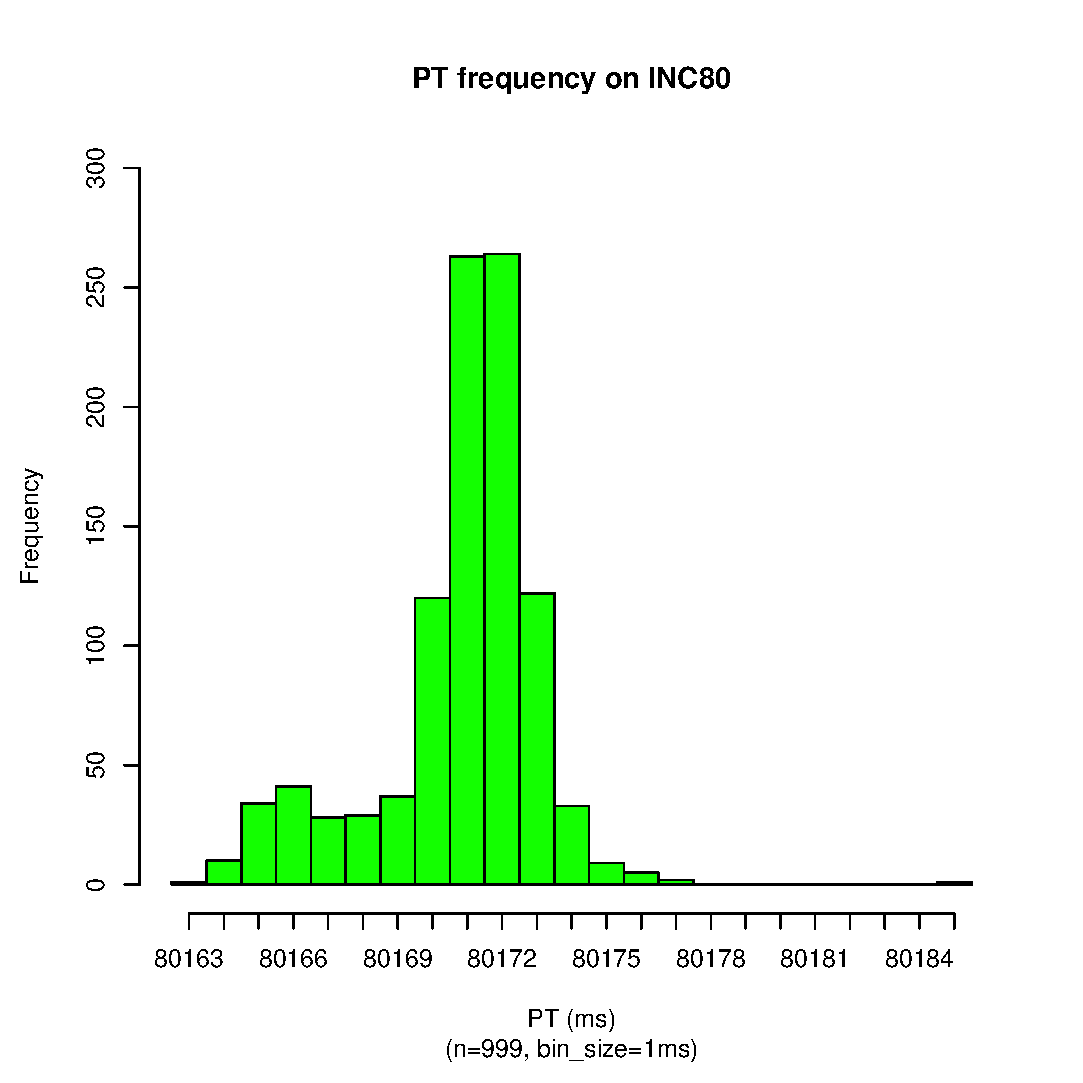
\includegraphics[scale=0.43]{u_s_time/80_sec_pt_hist.eps}
		\label{fig:inc80_pt_hist}
	}
	\subfigure[PT frequency on INC88 on {\tt sodb9}]{
		\includegraphics[scale=0.43]{u_s_time/88_sec_pt_hist.eps}
		\label{fig:inc88_pt_hist}
	}
	\caption{PT Histograms of INC48 ... INC88~\label{fig:new_pt_hist2}}
\end{figure}

\pagebreak
\newpage

\begin{figure}[hp!]
	\centering
	\subfigure[PT frequency on INC96 on {\tt sodb9}]{
		\includegraphics[scale=0.43]{u_s_time/96_sec_pt_hist.eps}
		\label{fig:inc96_pt_hist}
	}
	\subfigure[PT frequency on INC104 on {\tt sodb9}]{
		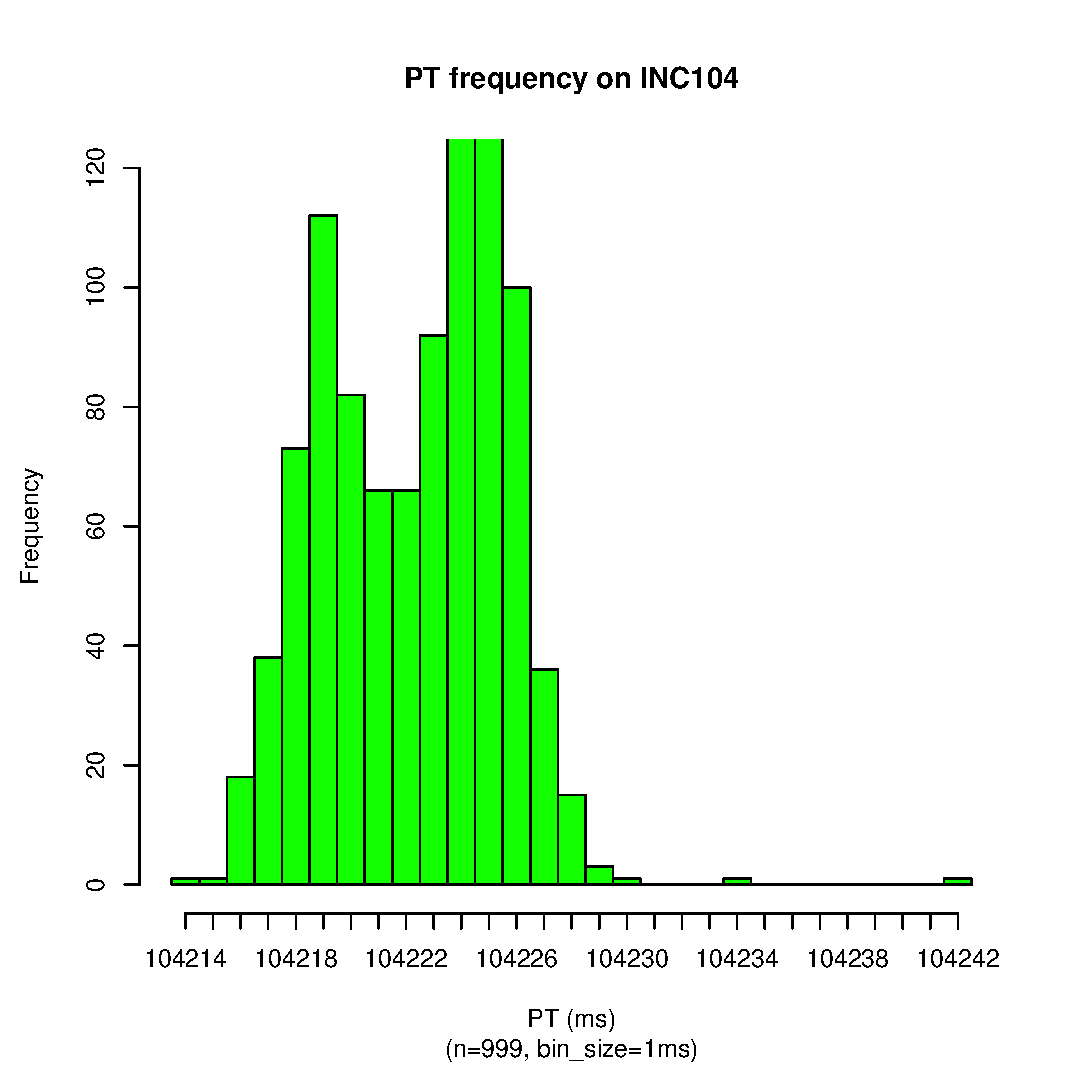
\includegraphics[scale=0.43]{u_s_time/104_sec_pt_hist.eps}
		\label{fig:inc104_pt_hist}
	}
	\subfigure[PT frequency on INC112 on {\tt sodb9}]{
		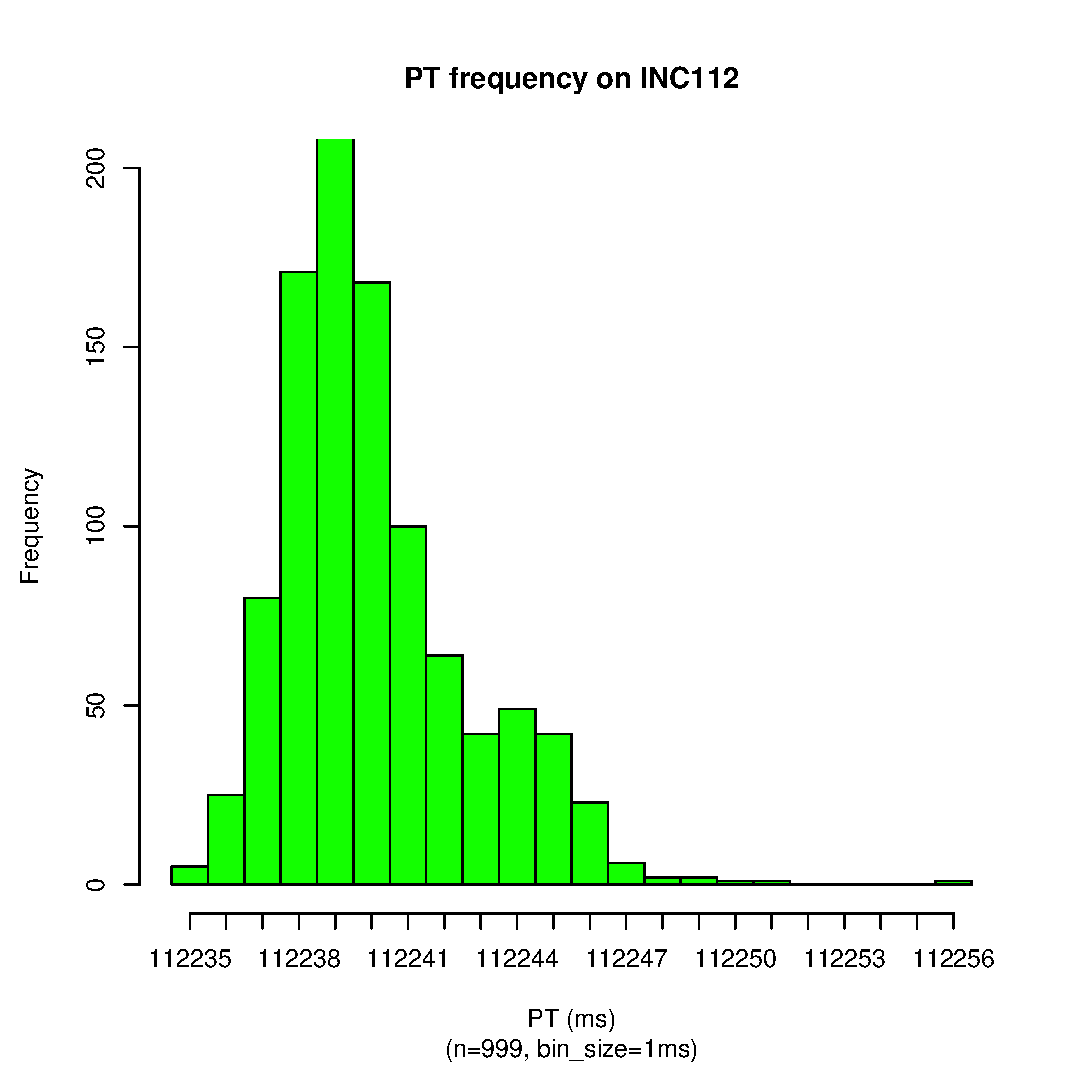
\includegraphics[scale=0.43]{u_s_time/112_sec_pt_hist.eps}
		\label{fig:inc112_pt_hist}
	}
	\subfigure[PT frequency on INC120 on {\tt sodb9}]{
		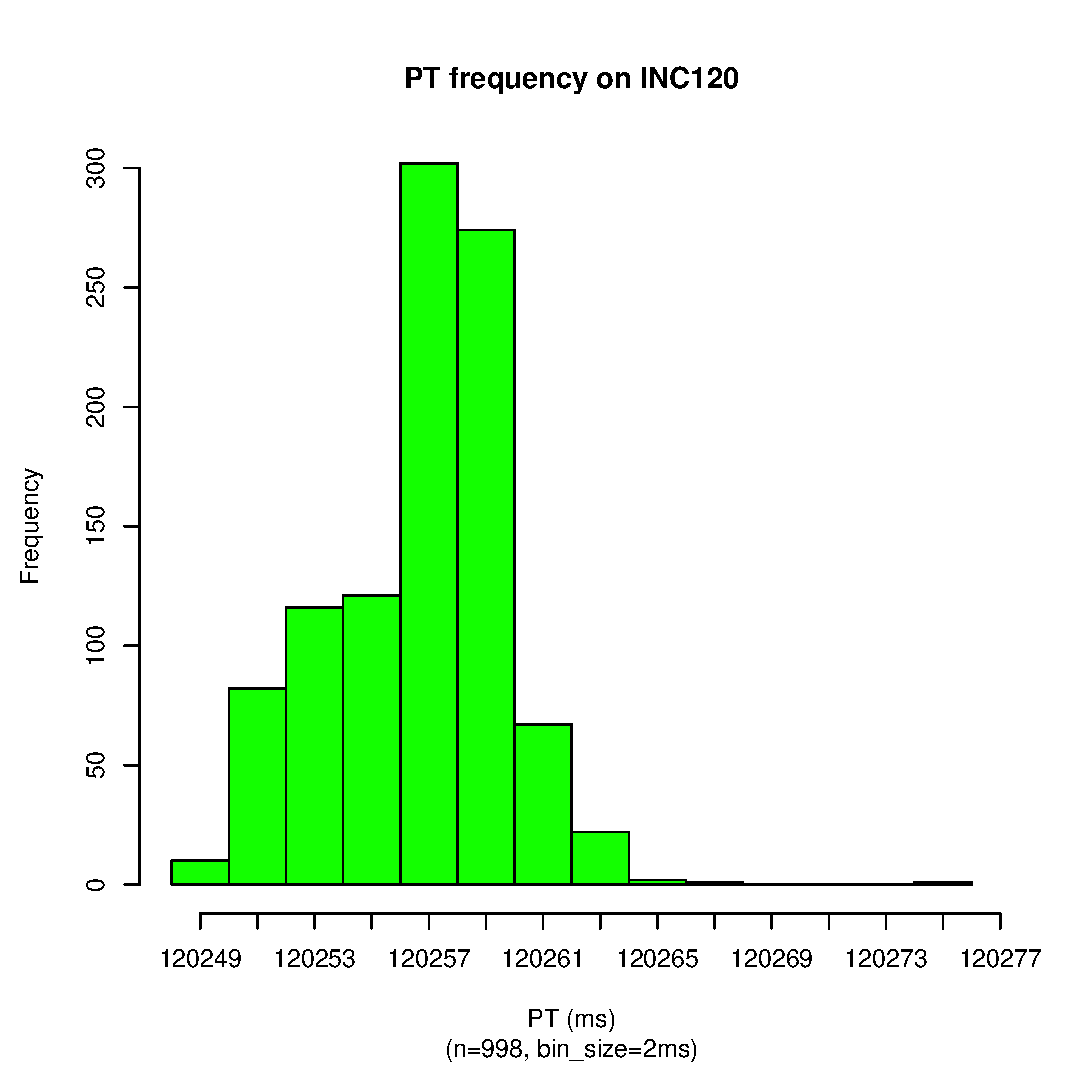
\includegraphics[scale=0.43]{u_s_time/120_sec_pt_hist.eps}
		\label{fig:inc120_pt_hist}
	}
	\caption{PT Histograms of INC96 ... INC120~\label{fig:new_pt_hist3}}
\end{figure}

\pagebreak
\newpage

\begin{figure}[hp!]
	\centering
	\subfigure[PT frequency on INC160 on {\tt sodb9}]{
		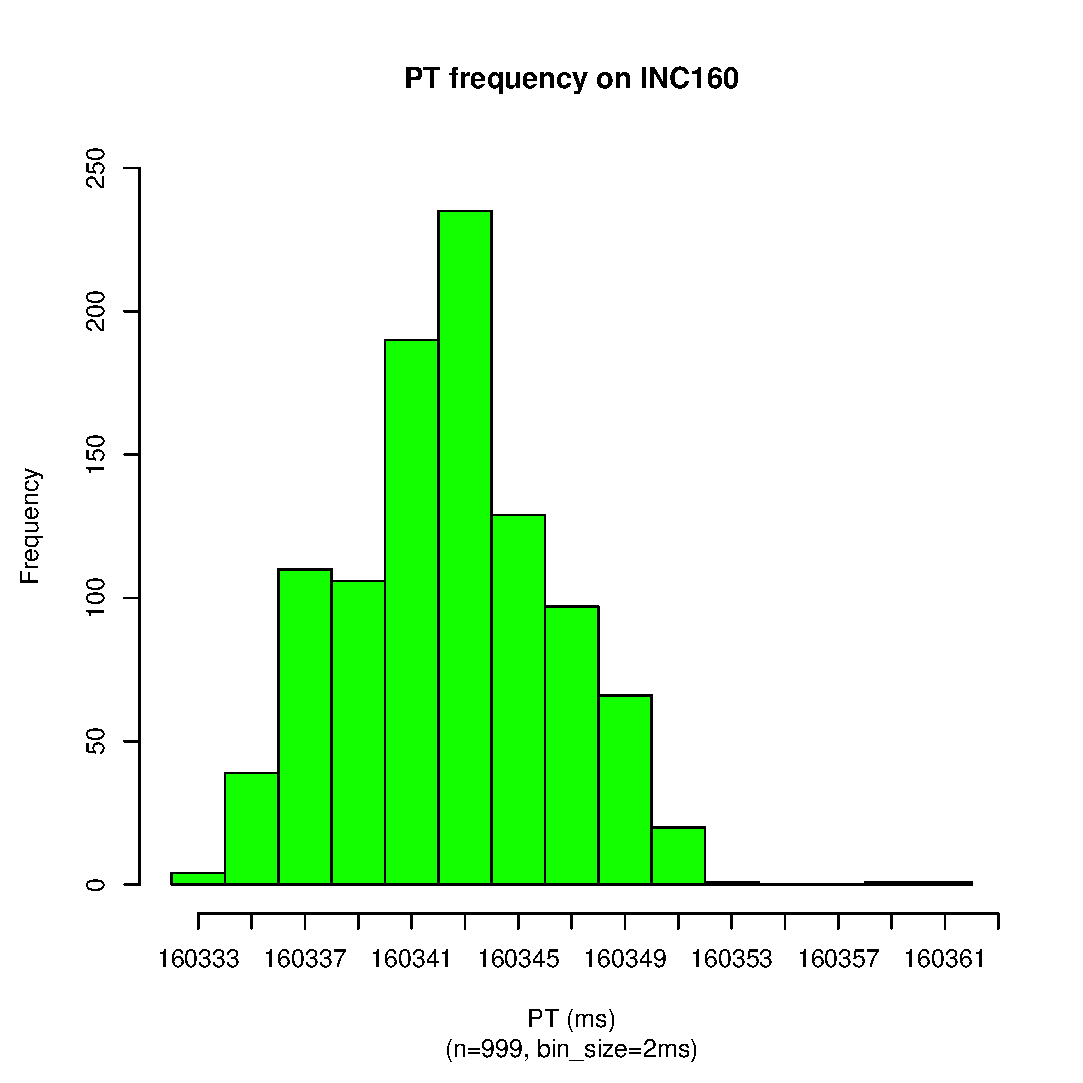
\includegraphics[scale=0.43]{u_s_time/160_sec_pt_hist.eps}
		\label{fig:inc160_pt_hist}
	}
	\subfigure[PT frequency on INC192 on {\tt sodb9}]{
		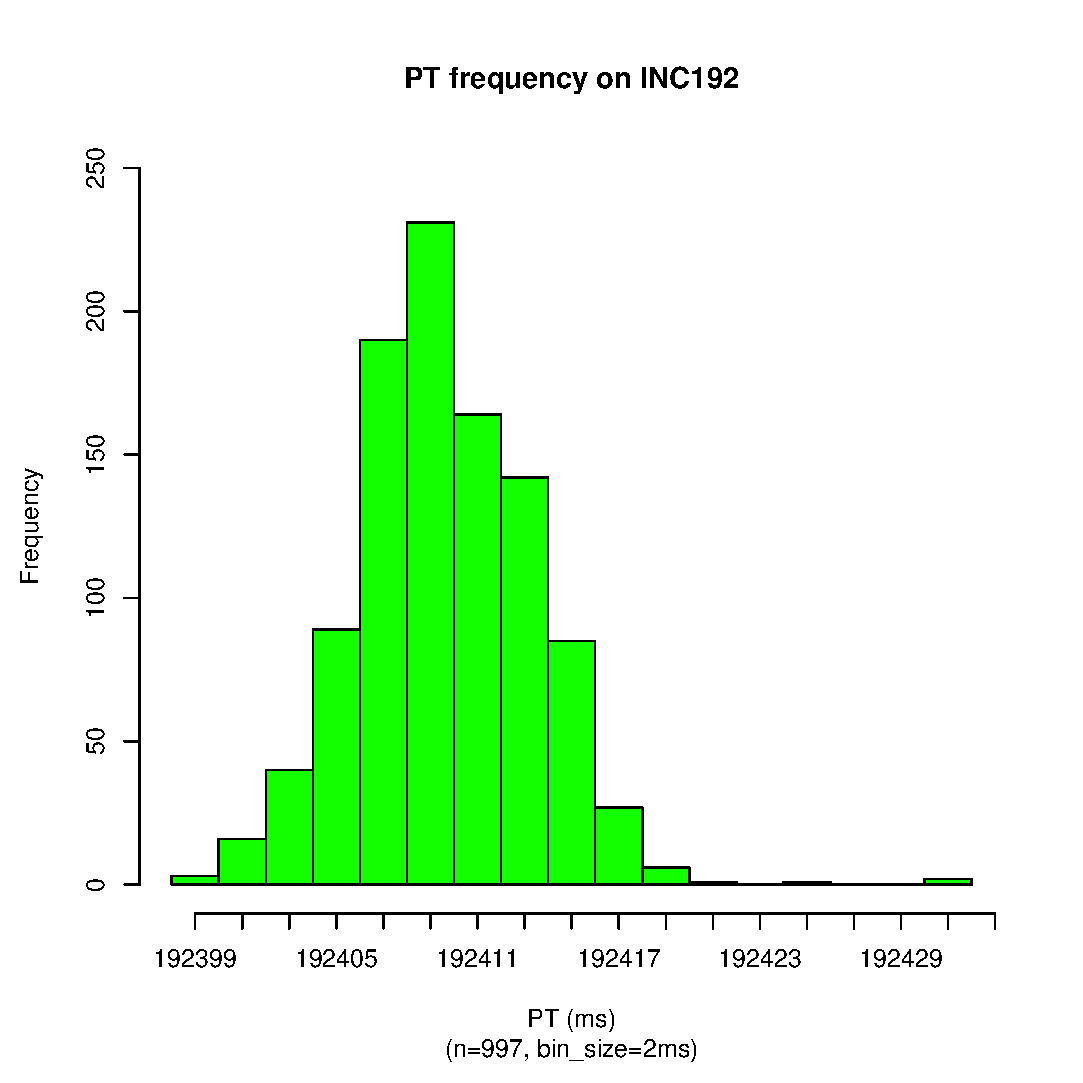
\includegraphics[scale=0.43]{u_s_time/192_sec_pt_hist.eps}
		\label{fig:inc192_pt_hist}
	}
	\subfigure[PT frequency on INC224 on {\tt sodb9}]{
		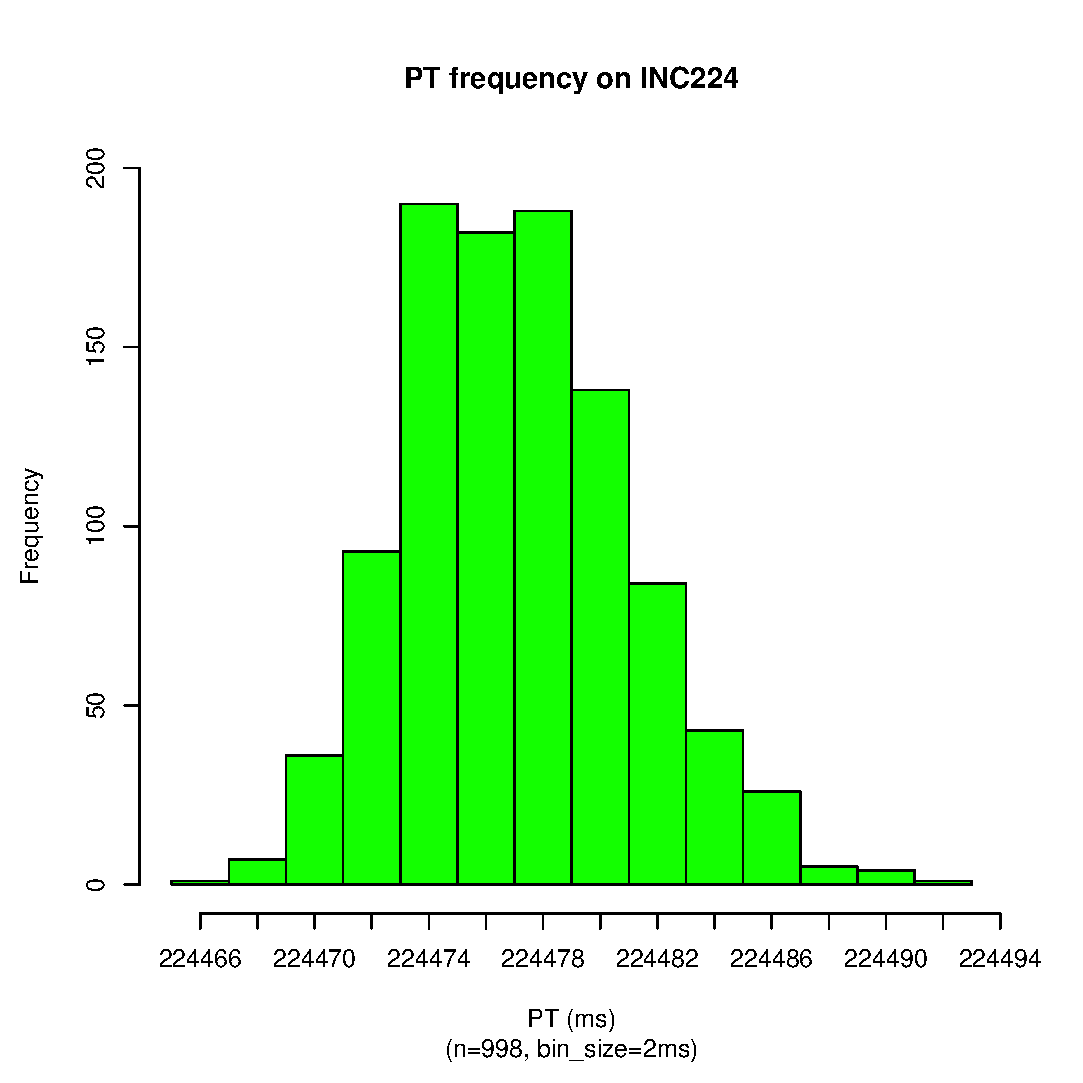
\includegraphics[scale=0.43]{u_s_time/224_sec_pt_hist.eps}
		\label{fig:inc224_pt_hist}
	}
	\caption{PT Histograms of INC169 ... INC224~\label{fig:new_pt_hist4}}
\end{figure}

\pagebreak
\newpage

\subsection{Summary}

\paragraph{Stacked Histograms in a 3D Plot:}
Figure~\ref{fig:hist3d} represents a 3D plot of collecting the histograms of PT in Section~\ref{sec:1st_pt}. 
Note that we additionally include the histograms from the task lengths of 8192 and 16384 seconds, which will be shown in Figures~\ref{fig:inc8192_r2_hist_v5} and~\ref{fig:inc16384_r2_hist_v5} (on page~47). See the legend in the right hand side of the figure, for more details about specific task length information. 
(To obtain the better shape, we could remove from those histograms the outliers that are identified via the second step of EMPv5.)
The x-axis corresponds to the normalized PT relative to the minimum, ranging 0 to 100, the y-axis to task length in log scale, and the z-axis to the normalized frequency relative to the highest bar for each histogram.

One thing to notice is that there are some runs having a few empty bins 
in their respective histogram. For instance, INC32 has such an empty bin as shown in Figure~\ref{fig:inc32_r1_et_hist_v5}. 
Same with INC256 in Figure~\ref{fig:inc256_r1_et_hist_v5}. For such an INC run, the z-axis associated with its histogram has the zero value on the x-axis in Figure~\ref{fig:hist3d}. 

\begin{figure}[htp!]
%\vspace{-.3in}
	\centering
	%\includegraphics[scale=0.6,angle=270]{u_s_time/3d_plot.eps}\label{fig:3d_plot}
	%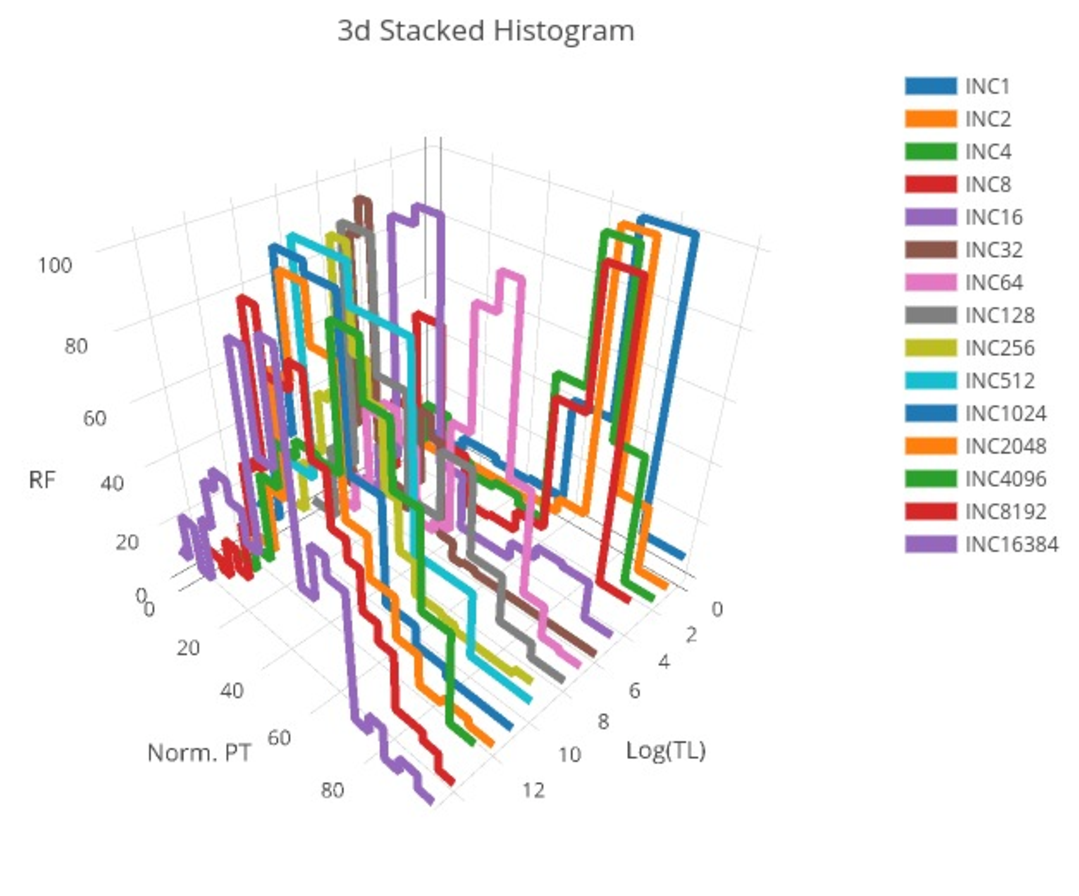
\includegraphics[scale=0.6]{u_s_time/new_3d_plot}\label{fig:3d_plot}
	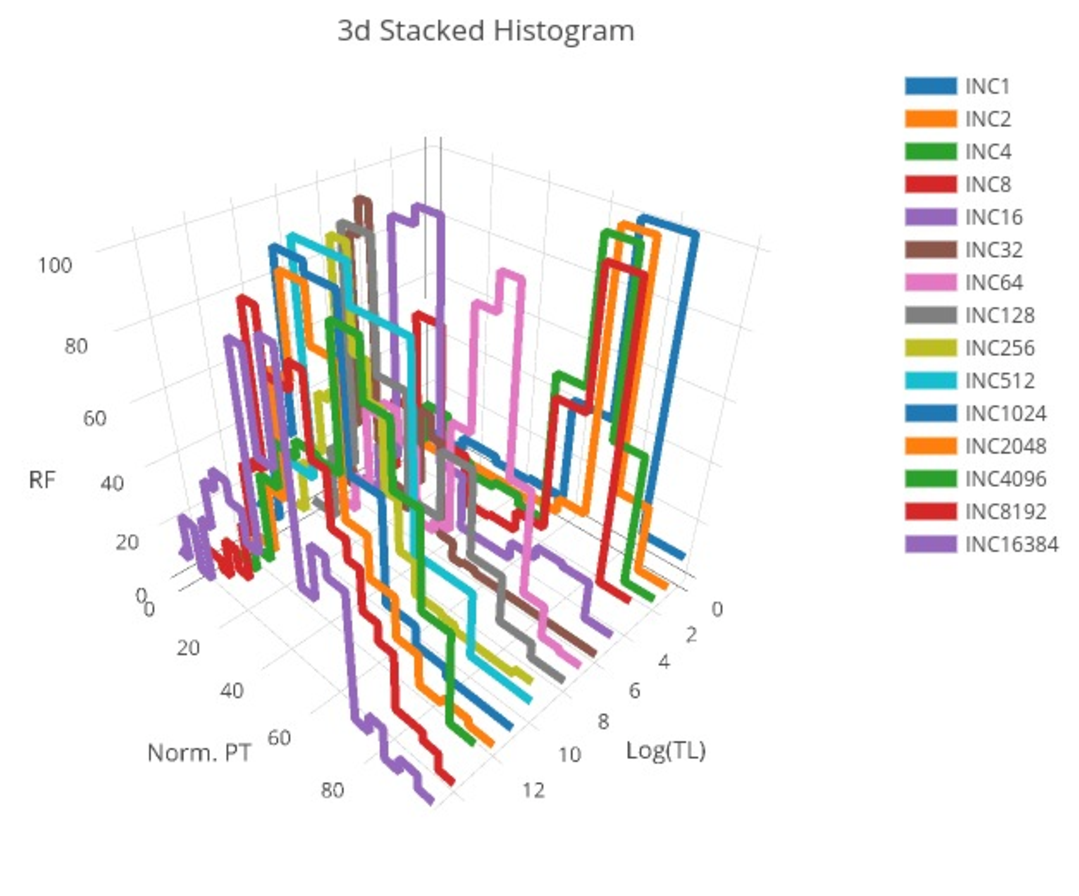
\includegraphics[scale=1]{u_s_time/new_3d_plot}\label{fig:3d_plot}
	\caption{3D histograms of PT on doubly-increasing INC on {\tt sodb9} for up to INC1024, on {\tt sodb10} for INC2048, on {\tt sodb12} for INC4096~\label{fig:hist3d}}
\end{figure}

\pagebreak
\clearpage
Figure~\ref{fig:hist3d_u} represents a 3D plot of collecting the histograms of user time only
exhibited in Section~\ref{sec:first_run}. 
\begin{figure}[htp!]
%\vspace{-.3in}
	\centering
	\includegraphics[scale=1]{u_s_time/3dplot_utime_only}\label{fig:3d_plot_u}
	\caption{3D histograms on INC on {\tt sodb9} for up to INC1024, on {\tt sodb10} for INC2048, on {\tt sodb12} for INC4096: user time only~\label{fig:hist3d_u}}
\end{figure}

\clearpage
\pagebreak

\paragraph{Fitting PT Histograms in Bi-Normal Distributions:}
We ran Rob's code to obtain a bi-normal fit for each INC's PT histogram 
in Section~\ref{sec:first_run}. 
Table~\ref{tab:binormal_fit} exhibits the total range of bins, the two means (modes), standard deviations, scales (weights) 
for the PT histogram, and figure numbers associated with each INC.

\begin{table}[h]
\begin{center}
\begin{tabular}{|l|l|l|l|l|l|l|l|l|} \hline
INC        & Total Range & Mean 1 & Mean 2 & Std 1 & Std 2 & Scale 1 & Scale 2 & Figures \\ \hline
INC1      & 6 & 1.66  & 4.73 & 1.03 & 0.54 & 0.10 & 0.90  & Fig.~\ref{fig:inc1_r1_hist_v5}\\ \hline
INC2      & 9 & 2.33  & 7.07 & 2.38 & 0.54 & 0.16 & 0.84  & Fig.~\ref{fig:inc2_r1_hist_v5} \\ \hline
INC4      & 9 & 2.17  & 7.89 & 0.99 & 0.86 & 0.21 & 0.79  & Fig.~\ref{fig:inc4_r1_hist_v5} \\ \hline
INC8      & 9 & 3.51  & 9.15 & 1.10 & 1.08 & 0.39 & 0.61  & Fig.~\ref{fig:inc8_r1_hist_v5}\\ \hline
INC16    & 10 & 4.04  & 9.53 & 0.98 & 1.28 & 0.83 & 0.17  & Fig.~\ref{fig:inc16_r1_hist_v5}\\ \hline
INC32    & 22 & 2.76  & 8.26 & 1.28 & 1.12 & 0.73 & 0.27  & Fig.~\ref{fig:inc32_r1_hist_v5}\\ \hline
INC64    & 14 & 6.36  & 12.02 & 1.64 & 1.62 &  0.35 & 0.65  & Fig.~\ref{fig:inc64_r1_hist_v5}\\ \hline
INC128  & 16 & 4.21  & 8.64 & 1.82 & 3.40 & 0.41 & 0.59  & Fig.~\ref{fig:inc128_r1_hist_v5}\\ \hline
INC256  & 38 & 6.08  & 14.61  & 3.59 & 3.75 & 0.12 & 0.88  & Fig.~\ref{fig:inc256_r1_hist_v5}\\ \hline
INC512  & 20 & 1.60  & 12.43   & 11.51 & 4.47 & 0.08 & 0.92  & Fig.~\ref{fig:inc512_r1_hist_v5}\\ \hline
INC1024 & 40 & 1.13  & 18.88  & 14.99 & 6.01 & 0.06 & 0.94 & Fig.~\ref{fig:inc1024_r1_hist_v5}\\ \hline
INC2048 & 65 & 29.93 & 52.92 & 8.53 & 6.59 & 1.00 & -0.00 & Fig.~\ref{fig:inc2048_r1_hist_v5}\\ \hline
INC4096 & 65 & 39.57 & 98.00 & 12.41 & 8.19 & 0.94 & 0.06  & Fig.~\ref{fig:inc4096_r1_hist_v5}\\ \hline
\end{tabular}
\end{center}
\vspace{-.2in}
\caption{Two means in mode computed for each INC~\label{tab:binormal_fit}}
\end{table}

\pagebreak
\clearpage

\begin{figure}[htp!]
	\centering
	\subfigure[Mean]{
		\includegraphics[scale=0.6]{u_s_time/binormal_fit_mean.eps}
		\label{fig:binormal_mean}
	}
	\subfigure[Standard Deviation]{
		\includegraphics[scale=0.6]{u_s_time/binormal_fit_std.eps}
		\label{fig:binormal_std}
	}
	\subfigure[Scale]{
		\includegraphics[scale=0.6]{u_s_time/binormal_fit_scale.eps}
		\label{fig:binormal_scale}
	}
	\caption{Plots of two means, standard deviations, and scales for each INC 
	over increasing task length: based on Table~\ref{tab:binormal_fit}\label{fig:bnormal_Fit}}
\end{figure}

\clearpage
\pagebreak

%\subsection{Absolute and Relative Variance over Increasing Task Lengths}
\paragraph{Absolute and Relative Variance over Increasing Task Lengths:}
Figure~\ref{fig:cv_inc} exhibits absolute and relative variances over increasing task lengths. 
More specifically, Figures~\ref{fig:overall_std} and~\ref{fig:overall_std_log} 
concern the PT standard deviations of all the runs including those two longest runs of INC8192 and INC16384 described in Table~\ref{tab:exp_notes2}. 
The x-axis is task length, and the y-axis standard deviation; Figure~\ref{fig:overall_std_log} is taken in log scale.
Figures~\ref{fig:overall_re} and~\ref{fig:overall_re2} shows 
the relative variance of the same data set---{\em coefficient of variation} (= standard deviation 
/ task length (or mean)). Both of the x and y axes in these two figures are taken in log scale. 
We also overlap a linear-square-fit of each case on the same figure. 

\begin{figure}[htp!]
	\centering
	\subfigure[Standard deviation (absolute)]{
		%\includegraphics[scale=0.6]{u_s_time/overall_std.eps}
		\includegraphics[scale=0.6]{u_s_time/new_overall_pt_std.eps}
		\label{fig:overall_std}
	}
	\subfigure[Standard deviation (absolute) in log scale]{
		%\includegraphics[scale=0.6]{u_s_time/overall_std_log.eps}
		\includegraphics[scale=0.6]{u_s_time/new_overall_pt_std_log.eps}
		\label{fig:overall_std_log}
	}
	\subfigure[Coefficient of variation in log scale (relative): divisor=mean]{
		\includegraphics[scale=0.6]{u_s_time/overall_pt_re.eps}
		\label{fig:overall_re}
	}
	\subfigure[Coefficient of variation in log scale (relative): divisor=task length]{
		\includegraphics[scale=0.6]{u_s_time/new_overall_pt_re.eps}
		\label{fig:overall_re2}
	}
	\caption{Absolute and relative variances~\label{fig:cv_inc}}
\end{figure}



\pagebreak
\newpage

\section{Further Investigation of the Existing Runs and Some Additional Runs~\label{sec:u_s_time_hist}} 
This section exhibits user and system time histograms on the first run of 
INC with its task length increasing from 1 second to 1024 seconds 
and the second run of INC from 2048 seconds to 16384 seconds via EMPv5 with no Step 2.
The detailed description of the base data is from Table~\ref{tab:exp_notes1}, 
and for some additional data, the corresponding description is given in Table~\ref{tab:exp_notes4}.

\begin{table}[h]
\begin{center}
\begin{tabular}{|p{2cm}|p{3cm}|p{3cm}|p{4cm}|p{3.5cm}|} \hline
Machine & Task Length (sec) & Description & Experiment Period & Relevant \linebreak Histograms\\ \hline
{\tt sodb9} &  INC96$\sim$INC256 & 1000 samples, each & 2017-05-24 $\sim$ 2017-06-06 & 
Figs.~\ref{fig:ut_hist3}, \ref{fig:inc224_ut_hist}, and~\ref{fig:inc256_ut_hist}\\ \hline
					&  INC3, 6, 12, 24, 48, 72, 80, 88, 104, 112, and 120 & 1000 samples, each & 2017-06-07 $\sim$ 2017-06-16 & Figs.~\ref{fig:inc3_ut_hist}, ~\ref{fig:inc6_ut_hist}, ~\ref{fig:inc12_ut_hist}, ~\ref{fig:inc24_ut_hist},
~\ref{fig:inc48_ut_hist}, ~\ref{fig:inc72_ut_hist}, ~\ref{fig:inc80_ut_hist}, ~\ref{fig:inc88_ut_hist}, ~\ref{fig:inc104_ut_hist},~\ref{fig:inc112_ut_hist}, and~\ref{fig:inc120_ut_hist}\\ \hline
%%%%% INC2048 and INC4096 come from the second run
\end{tabular}
\end{center}
\vspace{-.2in}
\caption{Notes on experiment runs used for histograms\label{tab:exp_notes4}}
\end{table}

\subsection{Summary of Histograms}

\begin{figure}[htp!]
\vspace{-.3in}
	\centering
	\includegraphics[scale=0.6,angle=270]{u_s_time/3d_plot.eps}\label{fig:3d_plot}
	\caption{3D histograms on INC~\label{fig:hist3d}}
\end{figure}

\clearpage
\pagebreak

\subsection{Absolute and Relative Variance over Increasing Task Length}

\begin{figure}[htp!]
	\centering
	\subfigure[Standard deviation (absolute)]{
		%\includegraphics[scale=0.6]{u_s_time/overall_std.eps}
		\includegraphics[scale=0.6]{u_s_time/new_overall_pt_std.eps}
		\label{fig:overall_std}
	}
	\subfigure[Standard deviation (absolute) in log scale]{
		%\includegraphics[scale=0.6]{u_s_time/overall_std_log.eps}
		\includegraphics[scale=0.6]{u_s_time/new_overall_pt_std_log.eps}
		\label{fig:overall_std_log}
	}
	\subfigure[Coefficient of variation in log scale (relative)]{
		\includegraphics[scale=0.6]{u_s_time/overall_re.eps}
		\label{fig:overall_re}
	}
	\subfigure[Coefficient of variation in log scale (relative): divisor=task length]{
		\includegraphics[scale=0.6]{u_s_time/new_overall_pt_re.eps}
		\label{fig:overall_re2}
	}
	\caption{Absolute and relative variances~\label{fig:cv_inc}}
\end{figure}

\pagebreak
\newpage

\subsection{Additional Histograms}

\subsubsection{ET}
Not available at this point, due to the labshelf server's unavailability for the time being.

\subsubsection{PT}
The histograms of INC1 through INC4096 are 
the same as those of Figures~\ref{fig:s9_r1_pt_hist1},~\ref{fig:s9_r1_pt_hist2},~\ref{fig:s9_r1_pt_hist3}, and~\ref{fig:s9_r1_pt_hist4}. 
The following are the histograms of INC with some intermediate task lengths.

\begin{figure}[hp!]
	\centering
	\subfigure[PT frequency on INC3]{
		\includegraphics[scale=0.43]{u_s_time/3_sec_pt_hist.eps}
		\label{fig:inc3_pt_hist}
	}
	\subfigure[PT frequency on INC6]{
		\includegraphics[scale=0.43]{u_s_time/6_sec_pt_hist.eps}
		\label{fig:inc6_pt_hist}
	}
	\subfigure[PT frequency on INC12]{
		\includegraphics[scale=0.43]{u_s_time/12_sec_pt_hist.eps}
		\label{fig:inc12_pt_hist}
	}
	\subfigure[PT frequency on INC24]{
		\includegraphics[scale=0.43]{u_s_time/24_sec_pt_hist.eps}
		\label{fig:inc24_pt_hist}
	}
	\caption{PT Histograms of INC3 ... INC24~\label{fig:new_pt_hist1}}
\end{figure}

\pagebreak
\newpage

\begin{figure}[hp!]
	\centering
	\subfigure[PT frequency on INC48]{
		\includegraphics[scale=0.43]{u_s_time/48_sec_pt_hist.eps}
		\label{fig:inc48_pt_hist}
	}
	\subfigure[PT frequency on INC72]{
		\includegraphics[scale=0.43]{u_s_time/72_sec_pt_hist.eps}
		\label{fig:inc72_pt_hist}
	}
	\subfigure[PT frequency on INC80]{
		\includegraphics[scale=0.43]{u_s_time/80_sec_pt_hist.eps}
		\label{fig:inc80_pt_hist}
	}
	\subfigure[PT frequency on INC88]{
		\includegraphics[scale=0.43]{u_s_time/88_sec_pt_hist.eps}
		\label{fig:inc88_pt_hist}
	}
	\caption{PT Histograms of INC48 ... INC88~\label{fig:new_pt_hist2}}
\end{figure}

\pagebreak
\newpage

\begin{figure}[hp!]
	\centering
	\subfigure[PT frequency on INC96]{
		\includegraphics[scale=0.43]{u_s_time/96_sec_pt_hist.eps}
		\label{fig:inc96_pt_hist}
	}
	\subfigure[PT frequency on INC104]{
		\includegraphics[scale=0.43]{u_s_time/104_sec_pt_hist.eps}
		\label{fig:inc104_pt_hist}
	}
	\subfigure[PT frequency on INC112]{
		\includegraphics[scale=0.43]{u_s_time/112_sec_pt_hist.eps}
		\label{fig:inc112_pt_hist}
	}
	\subfigure[PT frequency on INC120]{
		\includegraphics[scale=0.43]{u_s_time/120_sec_pt_hist.eps}
		\label{fig:inc120_pt_hist}
	}
	\caption{PT Histograms of INC96 ... INC120~\label{fig:new_pt_hist3}}
\end{figure}

\pagebreak
\newpage

\begin{figure}[hp!]
	\centering
	\subfigure[PT frequency on INC160]{
		\includegraphics[scale=0.43]{u_s_time/160_sec_pt_hist.eps}
		\label{fig:inc160_pt_hist}
	}
	\subfigure[PT frequency on INC192]{
		\includegraphics[scale=0.43]{u_s_time/192_sec_pt_hist.eps}
		\label{fig:inc192_pt_hist}
	}
	\subfigure[PT frequency on INC224]{
		\includegraphics[scale=0.43]{u_s_time/224_sec_pt_hist.eps}
		\label{fig:inc224_pt_hist}
	}
	\caption{PT Histograms of INC169 ... INC224~\label{fig:new_pt_hist4}}
\end{figure}

\pagebreak
\newpage

\subsection{User Time}

\begin{figure}[hp!]
	\centering
	\subfigure[User time frequency on INC1]{
		\includegraphics[scale=0.43]{u_s_time/1_sec_ut_hist.eps}
		\label{fig:inc1_ut_hist}
	}
	\subfigure[User time frequency on INC2]{
		\includegraphics[scale=0.43]{u_s_time/2_sec_ut_hist.eps}
		\label{fig:inc2_ut_hist}
	}
	\subfigure[User time frequency on INC3]{
		\includegraphics[scale=0.43]{u_s_time/3_sec_ut_hist.eps}
		\label{fig:inc3_ut_hist}
	}
	\subfigure[User time frequency on INC4]{
		\includegraphics[scale=0.43]{u_s_time/4_sec_ut_hist.eps}
		\label{fig:inc4_ut_hist}
	}
	\caption{User Time Histograms of INC1 ... INC4~\label{fig:ut_hist1}}
\end{figure}

\begin{figure}[hp!]
	\centering
	\subfigure[User time frequency on INC6]{
		\includegraphics[scale=0.43]{u_s_time/6_sec_ut_hist.eps}
		\label{fig:inc6_ut_hist}
	}
	\subfigure[User time frequency on INC8]{
		\includegraphics[scale=0.43]{u_s_time/8_sec_ut_hist.eps}
		\label{fig:inc8_ut_hist}
	}
	\subfigure[User time frequency on INC12]{
		\includegraphics[scale=0.43]{u_s_time/12_sec_ut_hist.eps}
		\label{fig:inc12_ut_hist}
	}
	\subfigure[User time frequency on INC16]{
		\includegraphics[scale=0.43]{u_s_time/16_sec_ut_hist.eps}
		\label{fig:inc16_ut_hist}
	}
	\caption{User Time Histograms of INC6 ... INC16~\label{fig:ut_hist2}}
\end{figure}


\begin{figure}[hp!]
	\centering
	\subfigure[User time frequency on INC24]{
		\includegraphics[scale=0.43]{u_s_time/24_sec_ut_hist.eps}
		\label{fig:inc24_ut_hist}
	}
	\subfigure[User time frequency on INC32]{
		\includegraphics[scale=0.43]{u_s_time/32_sec_ut_hist.eps}
		\label{fig:inc32_ut_hist}
	}
	\subfigure[User time frequency on INC48]{
		\includegraphics[scale=0.43]{u_s_time/48_sec_ut_hist.eps}
		\label{fig:inc48_ut_hist}
	}
	\subfigure[User time frequency on INC64]{
		\includegraphics[scale=0.43]{u_s_time/64_sec_ut_hist.eps}
		\label{fig:inc64_ut_hist}
	}
	\caption{User Time Histograms of INC24 ... INC64~\label{fig:ut_hist3}}
\end{figure}

\begin{figure}[hp!]
	\centering
	\subfigure[User time frequency on INC72]{
		\includegraphics[scale=0.43]{u_s_time/72_sec_ut_hist.eps}
		\label{fig:inc72_ut_hist}
	}
	\subfigure[User time frequency on INC80]{
		\includegraphics[scale=0.43]{u_s_time/80_sec_ut_hist.eps}
		\label{fig:inc80_ut_hist}
	}
	\subfigure[User time frequency on INC88]{
		\includegraphics[scale=0.43]{u_s_time/88_sec_ut_hist.eps}
		\label{fig:inc88_ut_hist}
	}
	\subfigure[User time frequency on INC96]{
		\includegraphics[scale=0.43]{u_s_time/96_sec_ut_hist.eps}
		\label{fig:inc96_ut_hist}
	}
	\caption{User Time Histograms of INC72 ... INC96~\label{fig:ut_hist4}}
\end{figure}

\begin{figure}[hp!]
	\centering
	\subfigure[User time frequency on INC104]{
		\includegraphics[scale=0.43]{u_s_time/104_sec_ut_hist.eps}
		\label{fig:inc104_ut_hist}
	}
	\subfigure[User time frequency on INC112]{
		\includegraphics[scale=0.43]{u_s_time/112_sec_ut_hist.eps}
		\label{fig:inc112_ut_hist}
	}
	\subfigure[User time frequency on INC120 with bin size = 1 ms]{
		\includegraphics[scale=0.43]{u_s_time/120_sec_ut_hist1.eps}
		\label{fig:inc120_ut_hist1}
	}
	\subfigure[User time frequency on INC120 with bin size = 2 ms]{
		\includegraphics[scale=0.43]{u_s_time/120_sec_ut_hist.eps}
		\label{fig:inc120_ut_hist}
	}
	\caption{User Time Histograms of INC104 and INC120~\label{fig:ut_hist5}}
\end{figure}

\begin{figure}[hp!]
	\centering
	\subfigure[User time frequency on INC128]{
		\includegraphics[scale=0.43]{u_s_time/128_sec_ut_hist2.eps}
		\label{fig:inc128_ut_hist2}
	}
	\subfigure[User time frequency on INC160]{
		\includegraphics[scale=0.43]{u_s_time/160_sec_ut_hist.eps}
		\label{fig:inc160_ut_hist}
	}
	\subfigure[User time frequency on INC192]{
		\includegraphics[scale=0.43]{u_s_time/192_sec_ut_hist.eps}
		\label{fig:inc192_ut_hist}
	}
	\subfigure[User time frequency on INC224]{
		\includegraphics[scale=0.43]{u_s_time/224_sec_ut_hist.eps}
		\label{fig:inc224_ut_hist}
	}
	\caption{User Time Histograms of INC160 ... INC224~\label{fig:ut_hist6}}
\end{figure}

\begin{figure}[hp!]
	\centering
	\subfigure[User time frequency on INC256]{
		\includegraphics[scale=0.43]{u_s_time/256_sec_ut_hist2.eps}
		\label{fig:inc256_ut_hist}
	}
	\subfigure[User time frequency on INC512 (with one extreme outlier of 513,259 msec removed)]{
		\includegraphics[scale=0.43]{u_s_time/512_sec_ut_hist.eps}
		\label{fig:inc512_ut_hist}
	}
	\subfigure[User time frequency on INC1024]{
		\includegraphics[scale=0.43]{u_s_time/1024_sec_ut_hist.eps}
		\label{fig:inc1024_ut_hist}
	}
	\caption{User Time Histograms of INC256 ... INC1024~\label{fig:ut_hist7}}
\end{figure}

\begin{figure}[hp!]
	\centering
	\subfigure[User time frequency on INC2048]{
		\includegraphics[scale=0.43]{u_s_time/2048_sec_ut_hist.eps}
		\label{fig:inc2048_ut_hist}
	}
	\subfigure[User time frequency on INC4096]{
		\includegraphics[scale=0.43]{u_s_time/4096_sec_ut_hist.eps}
		\label{fig:inc4096_ut_hist}
	}
	\caption{User Time Histograms of INC512 ... INC4096~\label{fig:ut_hist8}}
\end{figure}

\vspace\fill
\clearpage

\subsection{System Time}

\begin{figure}[hp!]
	\centering
	\subfigure[System time frequency on INC1]{
		\includegraphics[scale=0.43]{u_s_time/1_sec_st_hist.eps}
		\label{fig:inc1_hist_v5}
	}
	\subfigure[System time frequency on INC2]{
		\includegraphics[scale=0.43]{u_s_time/2_sec_st_hist.eps}
		\label{fig:inc2_hist_st}
	}
	\subfigure[System time frequency on INC4]{
		\includegraphics[scale=0.43]{u_s_time/4_sec_st_hist.eps}
		\label{fig:inc4_hist_st}
	}
	\subfigure[System time frequency on INC8]{
		\includegraphics[scale=0.43]{u_s_time/8_sec_st_hist.eps}
		\label{fig:inc8_hist_st}
	}
	\caption{System Time Histograms of INC1 ... INC8~\label{fig:st_hist1}}
\end{figure}

\begin{figure}[hp!]
	\centering
	\subfigure[System time frequency on INC16]{
		\includegraphics[scale=0.43]{u_s_time/16_sec_st_hist.eps}
		\label{fig:inc16_hist_st}
	}
	\subfigure[System time frequency on INC32]{
		\includegraphics[scale=0.43]{u_s_time/32_sec_st_hist.eps}
		\label{fig:inc32_hist_st}
	}
	\subfigure[System time frequency on INC64]{
		\includegraphics[scale=0.43]{u_s_time/64_sec_st_hist.eps}
		\label{fig:inc64_hist_st}
	}
	\caption{System Time Histograms of INC16 ... INC64\label{fig:st_hist2}}
\end{figure}

\begin{figure}[hp!]
	\centering
	\subfigure[System time frequency on INC128]{
		\includegraphics[scale=0.43]{u_s_time/128_sec_st_hist.eps}
		\label{fig:inc128_hist_st}
	}
	\subfigure[System time frequency on INC256]{
		\includegraphics[scale=0.43]{u_s_time/256_sec_st_hist.eps}
		\label{fig:inc256_hist_st}
	}
	\subfigure[System time frequency on INC512]{
		\includegraphics[scale=0.43]{u_s_time/512_sec_st_hist.eps}
		\label{fig:inc512_hist_st}
	}
	\subfigure[System time frequency on INC1024]{
		\includegraphics[scale=0.43]{u_s_time/1024_sec_st_hist.eps}
		\label{fig:inc1024_hist_st}
	}
	\caption{System Time Histograms of INC256 ... INC1024~\label{fig:st_hist3}}
\end{figure}

\begin{figure}[t]
	\centering
	\subfigure[System time frequency on INC2048]{
		\includegraphics[scale=0.43]{u_s_time/2048_sec_st_hist.eps}
		\label{fig:inc2048_hist_st}
	}
	\subfigure[System time frequency on INC4096]{
		\includegraphics[scale=0.43]{u_s_time/4096_sec_st_hist.eps}
		\label{fig:inc4096_hist_st}
	}
	\caption{System Time Histograms of INC2048 and INC4096~\label{fig:st_hist4}}
\end{figure}

\clearpage
\pagebreak

\subsection{Correlation}

\begin{table}[h]
\begin{center}
\begin{tabular}{|c|c|c|} \hline
 						   & INC2048's u time & INC2048's s time\\ \hline
INC2048's u time  &	 -  &  0.05\\ \hline					
daemon u time & 0.56 & 0.61\\ \hline
daemon s time & 0.48 & 0.57\\ \hline
daemon minor faults &  0.53 & 0.62\\ \hline
daemon major faults & 0.55 & 0.59 \\ \hline
daemon read bytes & 0.55 & 0.59 \\ \hline
daemon read char & 0.56 & 0.61\\ \hline
daemon read sys calls & 0.57 & 0.63\\ \hline
daemon write bytes & 0.57 &  0.64\\ \hline
daemon write char & 0.53 & 0.62\\ \hline
%write sys calls & N/A & N/A\\ \hline
\end{tabular}
\end{center}
\vspace{-.2in}
\caption{Correlation of user and system time of INC2048 with some daemon measures\label{tab:corr_table2}}
\end{table}

\begin{table}[h]
\begin{center}
\begin{tabular}{|c|c|c|} \hline
 						   & INC4096's u time & INC4096's s time\\ \hline
INC4096's u time  &	 -  & -0.30 \\ \hline					
daemon u time & 0.1 & {\bf 0.3} \\ \hline
daemon s time & -0.09 & {\bf 0.19} \\ \hline
daemon minor faults & {\bf 0.11} & {\bf 0.32} \\ \hline
%read bytes & N/A & N/A
daemon read char & 0.1 & {\bf 0.32} \\ \hline
daemon read sys calls & 0.11 & {\bf 0.32} \\ \hline
daemon write bytes & 0 & {\bf 0.26} \\ \hline
daemon write char & 0.11 & {\bf 0.32}\\ \hline
%write sys calls & N/A & N/A
\end{tabular}
\end{center}
\vspace{-.2in}
\caption{Correlation of user and system time of INC4096 with some daemon measures\label{tab:corr_table}}
\end{table}

\clearpage
\newpage

\subsection{Scatter Plots on Some Significant Correlations}
The following scatter plots correspond to the correlations bold in Table~\ref{tab:corr_table}.

\begin{figure}[htp!]
	\centering
	\subfigure[User time vs. Sum of all daemon system time]{
		\includegraphics[scale=0.43]{u_s_time/corr_u_as_time.eps}
		\label{fig:corr_u_as_time}
	}
	\subfigure[System time vs. Sum of all  daemon system time]{
		\includegraphics[scale=0.43]{u_s_time/corr_s_as_time.eps}
		\label{fig:corr_s_as_time}
	}
	\subfigure[User time vs. Sum of all  daemon minor faults]{
		\includegraphics[scale=0.43]{u_s_time/corr_mnf_u_time.eps}
		\label{fig:corr_u_mnf}
	}
	\subfigure[System time vs. Sum of all  daemon minor faults]{
		\includegraphics[scale=0.43]{u_s_time/corr_mnf_s_time.eps}
		\label{fig:corr_s_mnf}
	}
	\caption{Scatter plots between measures on INC4096~\label{fig:corr1}}
\end{figure}

\begin{figure}[htp!]
	\centering
	\subfigure[System time vs. Sum of all  daemon read char]{
		\includegraphics[scale=0.43]{u_s_time/corr_s_rchar.eps}
		\label{fig:corr_s_rchar}
	}
	\subfigure[System time vs. Sum of all  daemon read syscalls]{
		\includegraphics[scale=0.43]{u_s_time/corr_s_rsysc.eps}
		\label{fig:corr_s_rsysc}
	}
	\subfigure[System time vs. Sum of all  daemon write bytes]{
		\includegraphics[scale=0.43]{u_s_time/corr_s_wbytes.eps}
		\label{fig:corr_s_wbytes}
	}
	\subfigure[System time vs. Sum of all daemon write char]{
		\includegraphics[scale=0.43]{u_s_time/corr_s_wchar.eps}
		\label{fig:corr_s_wchar}
	}
	\caption{Scatter plots between measures on INC4096~\label{fig:corr2}}
\end{figure}

\clearpage

\subsection{Further Investigation of Some Samples}

\subsubsection{Samples in Fig.~\ref{fig:corr_u_mnf}}

\begin{table}[h]
\begin{center}
\begin{tabular}{|c|c|c|c|c|c|c|c|c|c|c|c|} \hline
proc name (id) & u time & s time & min flt & maj flt & r bytes & r char & r sysc & w bytes & w char & w sysc\\ \hline
INC4096 (3559) & 4103920 & 36 & 0 & 0 & 0 & 1 & 1 & 0 & 0 & 0 \\ \hline
proc\_monitor (25917) & 194 & 6 & 2 & 0 & 0 & 0 & 0 & 0 & 0 & 0 \\ \hline
md0\_raid1 (484) & 0 &  3 & 0 & 0 & 0 & 0 & 0 & 0 & 0 & 0 \\ \hline
java (3549) & 2 & 1 & 1093 & 0 & 0 & 11480 & 20 & 0 & 0 & 0 \\ \hline
cifsd (1927) & 0 & 1 & 0 & 0 & 0 & 0 & 0 & 0 & 0 & 0 \\ \hline
kblockd/0 (16) & 0 & 1 & 0 & 0 & 0 & 0 & 0 & 0 & 0 & 0 \\ \hline
ntpd (28232) & 0 & 1 & 1 & 0 & 0 & 0 & 42 & 4096 & 7 & 0 \\ \hline
\end{tabular}
\end{center}
\caption{Observed values of measures of processes on the leftmost sample in Fig.~\ref{fig:corr_u_mnf}~\label{tab:breakdown}}
\end{table}

\begin{table}[h]
\begin{center}
\begin{tabular}{|c|c|c|c|c|c|c|c|c|c|c|c|} \hline
proc name (id) & u time & s time & min flt & maj flt & r bytes & r char & r sysc & w bytes & w char & w sysc\\ \hline
INC4096 (3559) & 4103984 & 19 & 0 & 0 & 0 & 1 & 1 & 0 & 0 & 0 \\ \hline
proc\_monitor (25917) & 190 & 6 & 2 & 0 & 0 & 0 & 0 & 0 & 0 & 0 \\ \hline
java (3549) & 2 & 1 & 1093 & 0 & 0 & 11480 & 20 & 0 & 0 & 0 \\ \hline
md0\_raid1 (484) & 0 & 3 & 0 & 0 & 0 & 0 & 0 & 0 & 0 & 0 \\ \hline
ntpd (28232) & 0 & 0 & 1 & 0 & 0 & 0 & 39 & 4096 & 7 & 0 \\ \hline
java (4108) & 0 & 0  & 20 & 0 & 0 & 0 & 0 & 0 & 0 & 0 \\ \hline
\end{tabular}
\end{center}
\caption{Observed values of measures of processes on the second rightmost sample in Fig.~\ref{fig:corr_u_mnf}~\label{tab:breakdown2}}
\end{table}

\begin{table}[h]
\begin{center}
\begin{tabular}{|c|c|c|c|c|c|c|c|c|c|c|c|} \hline
proc name (id) & u time & s time & min flt & maj flt & r bytes & r char & r sysc & w bytes & w char & w sysc\\ \hline
INC4096 (3559) & 4103988 & 25 & 0 & 0 & 0 & 1 & 1 & 0 & 0 & 0 \\ \hline
proc\_monitor  (25917)  & 194 & 2 & 2 & 0 & 0 & 0 & 0 & 0 & 0 & 0 \\ \hline
sshd (3609) & 8 & 4 & 1382 & 0 & 0 & 512357 & 400 & 0 & 20881 & 0 \\ \hline
bash (3611)  & 4 & 1 & 835 & 0 & 0 & 283911 & 155 & 0 & 136 & 0 \\ \hline
md0\_raid1 (484) & 0 & 3 & 0 & 0 & 0 & 0 & 0 & 0 & 0 & 0 \\ \hline
java (3549) & 2 & 1 & 1093 & 0 & 0 & 11480 & 20 & 0 & 0 & 0 \\ \hline
cifsd (1927) & 0 & 2 & 0 & 0 & 0 & 0 & 0 & 0 & 0 & 0 \\ \hline
java (3606) & 0 & 1 & 22 & 0 & 0 & 0 & 0 & 0 & 0 & 0 \\ \hline
jbd2/md0-8 (497) & 0 & 1 & 0 & 0 & 0 & 0 & 0 & 450560 & 0 & 0 \\ \hline
kblockd/0 (16) & 0 & 1 & 0 & 0 & 0 & 0 & 0 & 0 & 0 & 0 \\ \hline
grep (3617) & 1 & 0 & 311 & 0 & 0 & 5417 & 11 & 0 & 0 & 0 \\ \hline
bash (3612) & 0 & 0 & 158 & 0 & 0 & 0 & 0 & 0 & 0 & 0 \\ \hline
consoletype (3613) & 0 & 0 & 127 & 0 & 0 & 1956 & 6 & 0 & 7 & 0 \\ \hline
bash (3614) & 0 & 0 & 174 & 0 & 0 & 0 & 0 & 0 & 0 & 0 \\ \hline
uname (3615) & 0 & 0 & 189 & 0 & 0 & 1956  & 6 & 0 & 7 & 0 \\ \hline
sshd (3610) & 0 & 0 & 425 & 0 & 0 & 22656 & 29 & 0 & 4630 & 0 \\ \hline
sshd (2105) & 0 & 0 & 14 & 0 & 0 & 0 & 0 & 0 & 594 & 0 \\ \hline
bash (3618) & 0 & 0 & 170 & 0 & 0 & 0 & 0 & 0 & 0 & 0 \\ \hline
id (3619) & 0 & 0 & 225 & 0 & 0 & 4352 & 12 & 0 & 2 & 0 \\ \hline
ntpd (28232) & 0 & 0 & 1 & 0 & 0 & 0 & 42 & 4096 & 7 & 0 \\ \hline
bash (3616) & 0 & 0 & 131 & 0 & 0 & 0 & 0 & 0 & 61 & 0 \\ \hline
\end{tabular}
\end{center}
\caption{Observed values of measures of processes on the rightmost sample in Fig.~\ref{fig:corr_u_mnf}~\label{tab:breakdown1}}
\end{table}

\clearpage
\newpage

\subsubsection{Samples in Fig.~\ref{fig:corr_s_wbytes}}

\begin{table}[h]
\begin{center}
\begin{tabular}{|c|c|c|c|c|c|c|c|c|c|c|c|} \hline
proc name (id) & u time & s time & min flt & maj flt & r bytes & r char & r sysc & w bytes & w char & w sysc\\ \hline
INC4096 (3559) & 4103981 & 14 & 0 & 0 & 0 & 1 & 1 & 0 & 0 & 0 \\ \hline
proc\_monitor (25917) & 194 & 2 & 2 & 0 & 0 & 0 & 0 & 0 & 0 & 0 \\ \hline
md0\_raid1 (484) & 0 & 5 & 0 & 0 & 0 & 0 & 0 & 0 & 0 & 0 \\ \hline
java (3549) & 2 & 1 & 1093 & 0 & 0 & 11480 & 20 & 0 & 0 & 0 \\ \hline
flush-9:0 (3548) & 0 & 2 & 0 & 0 & 0 & 0 & 0 & 0 & 0 & 0 \\ \hline
ntpd (28232) & 0 & 0 & 1 & 0 & 0 & 0 & 42 & 4096 & 7 & 0 \\ \hline
java (4585) & 0 & 0 & 20 & 0 & 0 & 0 & 0 & 0 & 0 & 0 \\ \hline
\end{tabular}
\end{center}
\caption{Observed values of measures of processes on the leftmost sample in Fig.~\ref{fig:corr_s_wbytes}~\label{tab:breakdown4}}
\end{table}

\begin{table}[h]
\begin{center}
\begin{tabular}{|c|c|c|c|c|c|c|c|c|c|c|c|} \hline
proc name (id) & u time & s time & min flt & maj flt & r bytes & r char & r sysc & w bytes & w char & w sysc\\ \hline
INC4096 (3559) & 4103958 & 44 & 0 & 0 & 0 & 1 & 1 & 0 & 0 & 0 \\ \hline
proc\_monitor (25917) & 194 & 2 & 2 & 0 & 0 & 0 & 0 & 0 & 0 & 0 \\ \hline
sshd (4877) & 10 & 4 & 1382 & 0 & 0 & 519568 & 392 & 0 & 20868 & 0 \\ \hline
sshd (4886) & 10 & 3 & 1383 & 0 & 0 & 515456 & 393 & 0 & 20868 & 0 \\ \hline
grep (4888) & 6 & 1 & 994 & 0 & 0 & 287034 & 154 & 0 & 136 & 0 \\ \hline
grep (4879) & 3 & 2 & 991 & 0 & 0 & 286801 & 159 & 0 & 136 & 0 \\ \hline
java (3549) & 2 & 1 & 1093 & 0 & 0 & 11480 & 20 & 0 & 0 & 0 \\ \hline
md0\_raid1 (484) & 0 & 3 & 0 & 0 & 0 & 0 & 0 & 0 & 0 & 0 \\ \hline
sshd (4878) & 2 & 1 & 424 & 0 & 0 & 22403 & 26 & 0 & 4268 & 0 \\ \hline
jbd2/md0-8 (497) & 0 & 2 & 0 & 0 & 0 & 0 & 0 & 696320 & 0 & 0 \\ \hline
flush-9:0 (3548) & 0 & 2 & 0 & 0 & 0 & 0 & 0 & 0 & 0 & 0 \\ \hline
cifsd (1927) & 0 & 1 & 0 & 0 & 0 & 0 & 0 & 0 & 0 & 0 \\ \hline
kblockd/0 (16) & 0 & 1 & 0 & 0 & 0 & 0 & 0 & 0 & 0 & 0 \\ \hline
grep (4892) & 0 & 1 & 309 & 0 & 0 & 5417 & 11 & 0 & 0 & 0 \\ \hline
grep (4883) & 1 & 0 & 310 & 0 & 0 & 5417 & 11 & 0 & 0 & 0 \\ \hline
id (4894) & 0 & 0 & 226 & 0 & 0 & 4352 & 12 & 0 & 2 & 0 \\ \hline
bash (4884) & 0 & 0 & 164 & 0 & 0 & 0 & 0 & 0 & 0 & 0 \\ \hline
id (4885) & 0 & 0 & 226 & 0 & 0 & 0 & 12 & 0 & 2 & 0 \\ \hline
sshd (2105) & 0 & 0 & 28 & 0 & 0 & 0 & 0 & 0 & 1188 & 0 \\ \hline
sshd (4887) & 0 & 0 & 425 & 0 & 0 & 22403 &26 & 0 & 4268 & 0 \\ \hline
ntpd (20232) & 0 & 0 & 1 & 0 & 0 & 0 & 42 & 4096 & 7 & 0 \\ \hline
bash (4880) & 0 & 0 & 165 & 0 & 0 & 0 & 0 & 0 & 0 & 0 \\ \hline
uname (4890)  & 0 & 0 & 190 & 0 & 0 & 1956  & 6 & 0 & 7 & 0 \\ \hline
bash (4891) & 0 & 0 & 128 & 0 & 0 & 0 & 0 & 0 & 61 & 0 \\ \hline
java  (4874) & 0 & 0 & 20 & 0 & 0 & 0 & 0 & 0 & 0 & 0 \\ \hline
bash (4893) & 0 & 0 & 164 & 0 & 0 & 0 & 0 & 0 & 0 & 0 \\ \hline
uname (4881)  & 0 & 0 & 191 & 0 & 0 & 1956  & 6 & 0 & 7 & 0 \\ \hline
bash (4889) & 0 & 0 & 165 & 0 & 0 & 0 & 0 & 0 & 0 & 0 \\ \hline
\end{tabular}
\end{center}
\caption{Observed values of measures of processes on the second rightmost sample in Fig.~\ref{fig:corr_s_wbytes}~\label{tab:breakdown5}}
\end{table}

\begin{table}[h]
\begin{center}
\begin{tabular}{|c|c|c|c|c|c|c|c|c|c|c|c|} \hline
proc name (id) & u time & s time & min flt & maj flt & r bytes & r char & r sysc & w bytes & w char & w sysc\\ \hline
INC4096 (3559) & 4103948 & 45 & 0 & 0 & 0 & 1 & 1 & 0 & 0 & 0 \\ \hline
proc\_monitor (25917) & 190 & 10 & 2 & 0 & 0 & 0 & 0 & 0 & 0 & 0 \\ \hline
md0\_raid1 (484) & 0 & 5 & 0 & 0 & 0 & 0 & 0 & 0 & 0 & 0 \\ \hline
jbd2/md0-8 (497) & 0 & 3 & 0 & 0 & 0 & 0 & 0 & 471040 & 0 & 0 \\ \hline
java (3549) & 2 & 1 & 1093 & 0 & 0 & 11480 & 20 & 0 & 0 & 0 \\ \hline
cifsd (1927) & 0 & 2 & 0 & 0 & 0 & 0 & 0 & 0 & 0 & 0 \\ \hline
flush-9:0 (3548) & 0 & 1 & 0 & 0 & 0 & 0 & 0 & 0 & 0 & 0 \\ \hline
java (5022) & 1 & 0 & 21 & 0 & 0 & 0 & 0 & 0 & 0 & 0 \\ \hline
ntpd (28232) & 0 & 0 & 1 & 0 & 0 & 0 & 42 & 4096 & 7 & 0 \\ \hline
\end{tabular}
\end{center}
\caption{Observed values of measures of processes on the rightmost sample in Fig.~\ref{fig:corr_s_wbytes}~\label{tab:breakdown6}}
\end{table}


\pagebreak
\newpage

\section{Histograms on the Second Run~\label{sec:sodb9_r2_hist}} 
This section exhibits histograms on the second run of 
INC with its task length increasing from 1 second to 4096 seconds, via SEDONA. 
The detailed description of the base data is from Table~\ref{tab:exp_notes2}.

\begin{table}[h]
\begin{center}
\begin{tabular}{|p{2cm}|p{3cm}|p{3cm}|p{4cm}|p{3.5cm}|} \hline
Machine & Task Length (sec) & Description & Experiment Period & Relevant \linebreak Histograms\\ \hline
{\tt sodb9} &  INC1$\sim$INC64 & 1000 samples, each & 2017-03-13 $\sim$ 2017-03-14 & Figs.~\ref{fig:s9_r2_et_hist1},~\ref{fig:s9_r2_et_hist2},~\ref{fig:s9_r2_pt_hist1}, and~\ref{fig:s9_r2_pt_hist2}\\ \hline
{\tt sodb9} &  INC128$\sim$INC1024 & 300 samples, each & 2017-03-14 $\sim$ 2017-03-21 & 
Figs.~\ref{fig:s9_r2_et_hist3} and~\ref{fig:s9_r2_pt_hist3}\\ \hline
{\tt sodb10} & INC2048 & 300 samples & 2017-03-13 $\sim$ 2017-03-20 & Figs.~\ref{fig:inc2048_r2_et_hist_v5} and~\ref{fig:inc2048_r2_hist_v5}\\ \hline
{\tt sodb12} & INC4096 & 300 samples & 2017-03-02 $\sim$ 2017-03-17 & Figs.~\ref{fig:inc4096_r2_et_hist_v5} and~\ref{fig:inc4096_r2_hist_v5}\\ \hline
\end{tabular}
\end{center}
\vspace{-.2in}
\caption{Notes on experiment runs used for histograms\label{tab:exp_notes2}}
\end{table}

\pagebreak

\subsection{ET}

\begin{figure}[hp!]
	\centering
	\subfigure[ET frequency on INC1]{
		\includegraphics[scale=0.43]{repet_data2/1_sec_et_hist_v5.eps}
		\label{fig:inc1_r2_et_hist_v5}
	}
	\subfigure[ET frequency on INC2]{
		\includegraphics[scale=0.43]{repet_data2/2_sec_et_hist_v5.eps}
		\label{fig:inc2_r2_et_hist_v5}
	}
	\subfigure[ET frequency on INC4]{
		\includegraphics[scale=0.43]{repet_data2/4_sec_et_hist_v5.eps}
		\label{fig:inc4_r2_et_hist_v5}
	}
	\subfigure[ET frequency on INC8]{
		\includegraphics[scale=0.43]{repet_data2/8_sec_et_hist_v5.eps}
		\label{fig:inc8_r2_et_hist_v5}
	}
	\caption{ET Histograms of INC1 ... INC8~\label{fig:s9_r2_et_hist1}}
\end{figure}

\begin{figure}[hp!]
	\centering
	\subfigure[ET frequency on INC16]{
		\includegraphics[scale=0.43]{repet_data2/16_sec_et_hist_v5.eps}
		\label{fig:inc16_r2_et_hist_v5}
	}
	\subfigure[ET frequency on INC32]{
		\includegraphics[scale=0.43]{repet_data2/32_sec_et_hist_v5.eps}
		\label{fig:inc32_r2_et_hist_v5}
	}
	\subfigure[ET frequency on INC64]{
		\includegraphics[scale=0.43]{repet_data2/64_sec_et_hist_v5.eps}
		\label{fig:inc64_r2_et_hist_v5}
	}
	\caption{ET Histograms of INC16 ... INC64~\label{fig:s9_r2_et_hist2}}
\end{figure}

\begin{figure}[hp!]
	\centering
	\subfigure[ET frequency on INC128]{
		\includegraphics[scale=0.43]{repet_data2/128_sec_et_hist_v5.eps}
		\label{fig:inc128_r2_et_hist_v5}
	}
	\subfigure[ET frequency on INC256]{
		\includegraphics[scale=0.43]{repet_data2/256_sec_et_hist_v5.eps}
		\label{fig:inc256_r2_et_hist_v5}
	}
	\subfigure[ET frequency on INC512]{
		\includegraphics[scale=0.43]{repet_data2/512_sec_et_hist_v5.eps}
		\label{fig:inc512_r2_et_hist_v5}
	}
	\subfigure[ET frequency on INC1024]{
		\includegraphics[scale=0.43]{repet_data2/1024_sec_et_hist_v5.eps}
		\label{fig:inc1024_r2_et_hist_v5}
	}
	\caption{ET Histograms of INC128 ... INC1024~\label{fig:s9_r2_et_hist3}}
\end{figure}

\begin{figure}[hp!]
	\centering
	\subfigure[ET frequency on INC2048]{
		\includegraphics[scale=0.43]{repet_data2/2048_sec_et_hist_v5.eps}
		\label{fig:inc2048_r2_et_hist_v5}
	}
	\subfigure[ET frequency on INC4096]{
		\includegraphics[scale=0.43]{repet_data2/4096_sec_et_hist_v5.eps}
		\label{fig:inc4096_r2_et_hist_v5}
	}
	\caption{ET Histograms of INC2048 and INC4096~\label{fig:s9_r2_et_hist4}}
\end{figure}

\vspace\fill
\clearpage

\subsection{PT}

\begin{figure}[hp!]
	\centering
	\subfigure[PT frequency on INC1]{
		\includegraphics[scale=0.43]{repet_data2/1_sec_pt_hist_v5.eps}
		\label{fig:inc1_r2_hist_v5}
	}
	\subfigure[PT frequency on INC2]{
		\includegraphics[scale=0.43]{repet_data2/2_sec_pt_hist_v5.eps}
		\label{fig:inc2_r2_hist_v5}
	}
	\subfigure[PT frequency on INC4]{
		\includegraphics[scale=0.43]{repet_data2/4_sec_pt_hist_v5.eps}
		\label{fig:inc4_r2_hist_v5}
	}
	\subfigure[PT frequency on INC8]{
		\includegraphics[scale=0.43]{repet_data2/8_sec_pt_hist_v5.eps}
		\label{fig:inc8_r2_hist_v5}
	}
	\caption{PT Histograms of INC1 ... INC8~\label{fig:s9_r2_pt_hist1}}
\end{figure}

\begin{figure}[hp!]
	\centering
	\subfigure[PT frequency on INC16]{
		\includegraphics[scale=0.43]{repet_data2/16_sec_pt_hist_v5.eps}
		\label{fig:inc16_r2_hist_v5}
	}
	\subfigure[PT frequency on INC32]{
		\includegraphics[scale=0.43]{repet_data2/32_sec_pt_hist_v5.eps}
		\label{fig:inc32_r2_hist_v5}
	}
	\subfigure[PT frequency on INC64]{
		\includegraphics[scale=0.43]{repet_data2/64_sec_pt_hist_v5.eps}
		\label{fig:inc64_r2_hist_v5}
	}
	\caption{PT Histograms of INC16 ... INC64\label{fig:s9_r2_pt_hist2}}
\end{figure}

\begin{figure}[hp!]
	\centering
	\subfigure[PT frequency on INC128]{
		\includegraphics[scale=0.43]{repet_data2/128_sec_pt_hist_v5.eps}
		\label{fig:inc128_r2_hist_v5}
	}
	\subfigure[PT frequency on INC256]{
		\includegraphics[scale=0.43]{repet_data2/256_sec_pt_hist_v5.eps}
		\label{fig:inc256_r2_hist_v5}
	}
	\subfigure[PT frequency on INC512]{
		\includegraphics[scale=0.43]{repet_data2/512_sec_pt_hist_v5.eps}
		\label{fig:inc512_r2_hist_v5}
	}
	\subfigure[PT frequency on INC1024]{
		\includegraphics[scale=0.43]{repet_data2/1024_sec_pt_hist_v5.eps}
		\label{fig:inc1024_r2_hist_v5}
	}
	\caption{PT Histograms of INC256 ... INC1024~\label{fig:s9_r2_pt_hist3}}
\end{figure}

\begin{figure}[t]
	\centering
	\subfigure[PT frequency on INC2048]{
		\includegraphics[scale=0.43]{repet_data2/2048_sec_pt_hist_v5.eps}
		\label{fig:inc2048_r2_hist_v5}
	}
	\subfigure[PT frequency on INC4096]{
		\includegraphics[scale=0.43]{repet_data2/4096_sec_pt_hist_v5.eps}
		\label{fig:inc4096_r2_hist_v5}
	}
	\caption{PT Histograms of INC2048 and INC4096~\label{fig:s9_r2_pt_hist4}}
\end{figure}

\clearpage
\pagebreak
\subsubsection{Analysis}
In this section we look into what happened inside the peaks observed in a certain histogram. 
We consider Figure~\ref{fig:inc8_r2_hist_v5} for this study. 
In the figure, we see the peaks at 8015 msec, 8020 msec, and 8021 msec. 

Table~\ref{tab:inc8_daemons} shows captured daemons and their runtime statistics per bin 
of figure. Note that bin is at the unit of PT. 
It appears that the peaks are definitely correlated with (1) appearances of some daemons 
and (2) times that those daemons co-ran with INC8. 

\begin{table}[h]
\begin{center}
{\scriptsize
\begin{tabular}{l|l|l|l|l|l|l|l} \hline
TASK\_LEN  & BIN (PT) &  DAEMON   & MIN\_PT  &  MAX\_PT  &  AVG\_PT  &   STD\_PT & Counts \\ \hline
INC8     & 8013  & jbd2/md0-8    & 1     & 1     & 1     & 0     & 1\\ \hline
INC8     & 8013  & kslowd000     & 1     & 1     & 1     & 0     & 1\\ \hline
INC8     & 8013  & md0\_raid1     & 1     & 1     & 1     & 0     & 17\\ \hline
INC8     & 8013  & proc\_monitor  & 196   & 200   & 197.72        & 1.07  & 18\\ \hline \hline

INC8     & 8014  & jbd2/md0-8    & 1     & 1     & 1     & 0     & 5\\ \hline
INC8     & 8014  & kslowd000     & 1     & 1     & 1     & 0     & 35\\ \hline
INC8     & 8014  & kslowd001     & 1     & 1     & 1     & 0     & 26\\ \hline
INC8     & 8014  & md0\_raid1     & 1     & 1     & 1     & 0     & 58\\ \hline
INC8     & 8014  & proc\_monitor  & 196   & 200   & 197.31        & 1.06  & 95\\ \hline \hline

INC8     & {\bf 8015}  & java  & 2     & 7     & 4.5   & 3.54  & 2\\ \hline
INC8     & {\bf 8015}  & jbd2/md0-8    & 1     & 1     & 1     & 0     & 2\\ \hline
INC8     & {\bf 8015}  & kslowd000     & 1     & 1     & 1     & 0     & 86\\ \hline
INC8     & {\bf 8015}  & kslowd001     & 1     & 1     & 1     & 0     & 89\\ \hline
INC8     & {\bf 8015}  & md0\_raid1     & 1     & 1     & 1     & 0     & 18\\ \hline
INC8     & {\bf 8015}  & proc\_monitor  & 196   & 200   & 197.28        & 1.01  & 194\\ \hline\hline

INC8     & 8016  & kslowd000     & 1     & 1     & 1     & 0     & 36\\ \hline
INC8     & 8016  & kslowd001     & 1     & 1     & 1     & 0     & 40\\ \hline
INC8     & 8016  & md0\_raid1     & 1     & 1     & 1     & 0     & 8\\ \hline
INC8     & 8016  & proc\_monitor  & 196   & 200   & 196.45        & .95   & 78\\ \hline\hline

INC8     & 8017  & kslowd000     & 1     & 1     & 1     & 0     & 11\\ \hline
INC8     & 8017  & kslowd001     & 1     & 1     & 1     & 0     & 10\\ \hline
INC8     & 8017  & md0\_raid1     & 1     & 1     & 1     & 0     & 3\\ \hline
INC8     & 8017  & proc\_monitor  & 196   & 200   & 197.15        & 1.16  & 26\\ \hline\hline

INC8     & 8018  & kslowd000     & 1     & 1     & 1     & 0     & 13\\ \hline
INC8     & 8018  & kslowd001     & 1     & 1     & 1     & 0     & 9\\ \hline
INC8     & 8018  & md0\_raid1     & 1     & 1     & 1     & 0     & 6\\ \hline
INC8     & 8018  & proc\_monitor  & 196   & 200   & 197.24        & 1.27  & 29\\ \hline\hline

INC8     & 8019  & jbd2/md0-8    & 1     & 1     & 1     & 0     & 3\\ \hline
INC8     & 8019  & kslowd000     & 1     & 1     & 1     & 0     & 9\\ \hline
INC8     & 8019  & kslowd001     & 1     & 2     & 1.06  & .24   & 18\\ \hline
INC8     & 8019  & md0\_raid1     & 1     & 1     & 1     & 0     & 27\\ \hline
INC8     & 8019  & proc\_monitor  & 196   & 200   & 197.1         & 1.18  & 52\\ \hline\hline

INC8     & {\bf 8020}  & jbd2/md0-8    & 1     & 1     & 1     & 0     & 8\\ \hline
INC8     & {\bf 8020}  & kslowd000     & 1     & 1     & 1     & 0     & 52\\ \hline
INC8     & {\bf 8020}  & kslowd001     & 1     & 1     & 1     & 0     & 57\\ \hline
INC8     & {\bf 8020}  & md0\_raid1     & 1     & 1     & 1     & 0     & 91\\ \hline
INC8     & {\bf 8020}  & proc\_monitor  & 196   & 200   & 197.03        & 1.02  & 180\\ \hline\hline

INC8     & {\bf 8021}  & cifsd         & 1     & 1     & 1     & 0     & 1\\ \hline
INC8     & {\bf 8021}  & java  & 2     & 37    & 19.5  & 24.75         & 2\\ \hline
INC8     & {\bf 8021}  & kslowd000     & 1     & 1     & 1     & 0     & 146\\ \hline
INC8     & {\bf 8021}  & kslowd001     & 1     & 1     & 1     & 0     & 143\\ \hline
INC8     & {\bf 8021}  & md0\_raid1     & 1     & 1     & 1     & 0     & 11\\ \hline
INC8     & {\bf 8021}  & proc\_monitor  & 196   & 198   & 197.15        & .98   & 299\\ \hline\hline

INC8     & 8022  & kslowd000     & 1     & 1     & 1     & 0     & 20\\ \hline
INC8     & 8022  & kslowd001     & 1     & 1     & 1     & 0     & 9\\ \hline
INC8     & 8022  & proc\_monitor  & 196   & 198   & 196.07        & .37   & 29\\ \hline\hline
\end{tabular}
}
\end{center}
\caption{Daemons observed from the INC8 run~\label{tab:inc8_daemons}}
\end{table}



\pagebreak
\newpage

\section{Histograms with 10,000 samples~\label{sec:sodb9_10k_hist}} 
This section exhibits histograms on two runs of 
INC, each with 8 and 16 seconds as its task length, having 10,000 repetitions.
The detailed description of the base data is from Table~\ref{tab:exp_notes3}.

\begin{table}[h]
\begin{center}
\begin{tabular}{|p{2cm}|p{3cm}|p{3cm}|p{4cm}|p{3.5cm}|} \hline
Machine & Task Length (sec) & Description & Experiment Period & Relevant \linebreak Histograms\\ \hline
{\tt sodb9} (plugged into {\em the upper left} power strip) &  INC8 & 10,000 samples & 2017-03-29 $\sim$ 2017-03-30 & Figs.~\ref{fig:inc8_10k_et_hist_v5} and~\ref{fig:inc8_10k_pt_hist_v5}\\ \hline
{\tt sodb10} (plugged into {\em the upper left} power strip) &  INC16 & 10,000 samples & 2017-03-29 $\sim$ 2017-03-31 & 
Figs.~\ref{fig:inc16_10k_et_hist_v5} and~\ref{fig:inc16_10k_pt_hist_v5}\\ \hline
\end{tabular}
\end{center}
\vspace{-.2in}
\caption{Notes on experiment runs used for histograms\label{tab:exp_notes3}}
\end{table}

\begin{figure}[hp!]
	\centering
	\subfigure[ET frequency on INC8 on {\tt sodb9}]{
		\includegraphics[scale=0.43]{10k_run/8_sec_et_hist_v5.eps}
		\label{fig:inc8_10k_et_hist_v5}
	}
	\subfigure[PT frequency on INC8 on {\tt sodb9}]{
		\includegraphics[scale=0.43]{10k_run/8_sec_pt_hist_v5.eps}
		\label{fig:inc8_10k_pt_hist_v5}
	}
	\subfigure[ET frequency on INC16 on {\tt sodb10}]{
		\includegraphics[scale=0.43]{10k_run/16_sec_et_hist_v5.eps}
		\label{fig:inc16_10k_et_hist_v5}
	}
	\subfigure[PT frequency on INC16 on {\tt sodb10}]{
		\includegraphics[scale=0.43]{10k_run/16_sec_pt_hist_v5.eps}
		\label{fig:inc16_10k_pt_hist_v5}
	}
	\caption{Histograms of INC8 and INC16 with 10,000 samples~\label{fig:10k_run_hist}}
\end{figure}


%\pagebreak
%\newpage
%
%\section{A Characterization Study on the First Run~\label{sec:sodb9_r3_hist}} 
This section further discusses the first run of 
INC with its task length increasing from 1 second to 4096 seconds via EMPv5 with no Step 2. 
The detailed description of the base data is from Table~\ref{tab:exp_notes1}.

\subsection{Summary of Histograms}

\begin{figure}[hp!]
\vspace{-.3in}
	\centering
	\includegraphics[scale=0.5,angle=270]{u_s_time/3d_plot.eps}\label{fig:3d_plot}
	\caption{3D histograms on INC~\label{fig:hist3d}}
\end{figure}

\subsection{Absolute and Relative Variance over Increasing Task Length}

\begin{figure}[hp!]
	\centering
	\subfigure[Standard deviation (absolute)]{
		\includegraphics[scale=0.6]{u_s_time/overall_std.eps}
		\label{fig:overall_std}
	}
	\subfigure[Coefficient of variation (relative)]{
		\includegraphics[scale=0.6]{u_s_time/overall_re.eps}
		\label{fig:overall_re}
	}
	\caption{Absolute and relative variances~\label{fig:cv_inc}}
\end{figure}

\pagebreak
\newpage

%\pagebreak
%\newpage
%
%\section{Further Investigation of the Existing Runs and Some Additional Runs~\label{sec:u_s_time_hist}} 
This section exhibits user and system time histograms on the first run of 
INC with its task length increasing from 1 second to 1024 seconds 
and the second run of INC from 2048 seconds to 16384 seconds via EMPv5 with no Step 2.
The detailed description of the base data is from Table~\ref{tab:exp_notes1}, 
and for some additional data, the corresponding description is given in Table~\ref{tab:exp_notes4}.

\begin{table}[h]
\begin{center}
\begin{tabular}{|p{2cm}|p{3cm}|p{3cm}|p{4cm}|p{3.5cm}|} \hline
Machine & Task Length (sec) & Description & Experiment Period & Relevant \linebreak Histograms\\ \hline
{\tt sodb9} &  INC96$\sim$INC256 & 1000 samples, each & 2017-05-24 $\sim$ 2017-06-06 & 
Figs.~\ref{fig:ut_hist3}, \ref{fig:inc224_ut_hist}, and~\ref{fig:inc256_ut_hist}\\ \hline
					&  INC3, 6, 12, 24, 48, 72, 80, 88, 104, 112, and 120 & 1000 samples, each & 2017-06-07 $\sim$ 2017-06-16 & Figs.~\ref{fig:inc3_ut_hist}, ~\ref{fig:inc6_ut_hist}, ~\ref{fig:inc12_ut_hist}, ~\ref{fig:inc24_ut_hist},
~\ref{fig:inc48_ut_hist}, ~\ref{fig:inc72_ut_hist}, ~\ref{fig:inc80_ut_hist}, ~\ref{fig:inc88_ut_hist}, ~\ref{fig:inc104_ut_hist},~\ref{fig:inc112_ut_hist}, and~\ref{fig:inc120_ut_hist}\\ \hline
%%%%% INC2048 and INC4096 come from the second run
\end{tabular}
\end{center}
\vspace{-.2in}
\caption{Notes on experiment runs used for histograms\label{tab:exp_notes4}}
\end{table}

\subsection{Summary of Histograms}

\begin{figure}[htp!]
\vspace{-.3in}
	\centering
	\includegraphics[scale=0.6,angle=270]{u_s_time/3d_plot.eps}\label{fig:3d_plot}
	\caption{3D histograms on INC~\label{fig:hist3d}}
\end{figure}

\clearpage
\pagebreak

\subsection{Absolute and Relative Variance over Increasing Task Length}

\begin{figure}[htp!]
	\centering
	\subfigure[Standard deviation (absolute)]{
		%\includegraphics[scale=0.6]{u_s_time/overall_std.eps}
		\includegraphics[scale=0.6]{u_s_time/new_overall_pt_std.eps}
		\label{fig:overall_std}
	}
	\subfigure[Standard deviation (absolute) in log scale]{
		%\includegraphics[scale=0.6]{u_s_time/overall_std_log.eps}
		\includegraphics[scale=0.6]{u_s_time/new_overall_pt_std_log.eps}
		\label{fig:overall_std_log}
	}
	\subfigure[Coefficient of variation in log scale (relative)]{
		\includegraphics[scale=0.6]{u_s_time/overall_re.eps}
		\label{fig:overall_re}
	}
	\subfigure[Coefficient of variation in log scale (relative): divisor=task length]{
		\includegraphics[scale=0.6]{u_s_time/new_overall_pt_re.eps}
		\label{fig:overall_re2}
	}
	\caption{Absolute and relative variances~\label{fig:cv_inc}}
\end{figure}

\pagebreak
\newpage

\subsection{Additional Histograms}

\subsubsection{ET}
Not available at this point, due to the labshelf server's unavailability for the time being.

\subsubsection{PT}
The histograms of INC1 through INC4096 are 
the same as those of Figures~\ref{fig:s9_r1_pt_hist1},~\ref{fig:s9_r1_pt_hist2},~\ref{fig:s9_r1_pt_hist3}, and~\ref{fig:s9_r1_pt_hist4}. 
The following are the histograms of INC with some intermediate task lengths.

\begin{figure}[hp!]
	\centering
	\subfigure[PT frequency on INC3]{
		\includegraphics[scale=0.43]{u_s_time/3_sec_pt_hist.eps}
		\label{fig:inc3_pt_hist}
	}
	\subfigure[PT frequency on INC6]{
		\includegraphics[scale=0.43]{u_s_time/6_sec_pt_hist.eps}
		\label{fig:inc6_pt_hist}
	}
	\subfigure[PT frequency on INC12]{
		\includegraphics[scale=0.43]{u_s_time/12_sec_pt_hist.eps}
		\label{fig:inc12_pt_hist}
	}
	\subfigure[PT frequency on INC24]{
		\includegraphics[scale=0.43]{u_s_time/24_sec_pt_hist.eps}
		\label{fig:inc24_pt_hist}
	}
	\caption{PT Histograms of INC3 ... INC24~\label{fig:new_pt_hist1}}
\end{figure}

\pagebreak
\newpage

\begin{figure}[hp!]
	\centering
	\subfigure[PT frequency on INC48]{
		\includegraphics[scale=0.43]{u_s_time/48_sec_pt_hist.eps}
		\label{fig:inc48_pt_hist}
	}
	\subfigure[PT frequency on INC72]{
		\includegraphics[scale=0.43]{u_s_time/72_sec_pt_hist.eps}
		\label{fig:inc72_pt_hist}
	}
	\subfigure[PT frequency on INC80]{
		\includegraphics[scale=0.43]{u_s_time/80_sec_pt_hist.eps}
		\label{fig:inc80_pt_hist}
	}
	\subfigure[PT frequency on INC88]{
		\includegraphics[scale=0.43]{u_s_time/88_sec_pt_hist.eps}
		\label{fig:inc88_pt_hist}
	}
	\caption{PT Histograms of INC48 ... INC88~\label{fig:new_pt_hist2}}
\end{figure}

\pagebreak
\newpage

\begin{figure}[hp!]
	\centering
	\subfigure[PT frequency on INC96]{
		\includegraphics[scale=0.43]{u_s_time/96_sec_pt_hist.eps}
		\label{fig:inc96_pt_hist}
	}
	\subfigure[PT frequency on INC104]{
		\includegraphics[scale=0.43]{u_s_time/104_sec_pt_hist.eps}
		\label{fig:inc104_pt_hist}
	}
	\subfigure[PT frequency on INC112]{
		\includegraphics[scale=0.43]{u_s_time/112_sec_pt_hist.eps}
		\label{fig:inc112_pt_hist}
	}
	\subfigure[PT frequency on INC120]{
		\includegraphics[scale=0.43]{u_s_time/120_sec_pt_hist.eps}
		\label{fig:inc120_pt_hist}
	}
	\caption{PT Histograms of INC96 ... INC120~\label{fig:new_pt_hist3}}
\end{figure}

\pagebreak
\newpage

\begin{figure}[hp!]
	\centering
	\subfigure[PT frequency on INC160]{
		\includegraphics[scale=0.43]{u_s_time/160_sec_pt_hist.eps}
		\label{fig:inc160_pt_hist}
	}
	\subfigure[PT frequency on INC192]{
		\includegraphics[scale=0.43]{u_s_time/192_sec_pt_hist.eps}
		\label{fig:inc192_pt_hist}
	}
	\subfigure[PT frequency on INC224]{
		\includegraphics[scale=0.43]{u_s_time/224_sec_pt_hist.eps}
		\label{fig:inc224_pt_hist}
	}
	\caption{PT Histograms of INC169 ... INC224~\label{fig:new_pt_hist4}}
\end{figure}

\pagebreak
\newpage

\subsection{User Time}

\begin{figure}[hp!]
	\centering
	\subfigure[User time frequency on INC1]{
		\includegraphics[scale=0.43]{u_s_time/1_sec_ut_hist.eps}
		\label{fig:inc1_ut_hist}
	}
	\subfigure[User time frequency on INC2]{
		\includegraphics[scale=0.43]{u_s_time/2_sec_ut_hist.eps}
		\label{fig:inc2_ut_hist}
	}
	\subfigure[User time frequency on INC3]{
		\includegraphics[scale=0.43]{u_s_time/3_sec_ut_hist.eps}
		\label{fig:inc3_ut_hist}
	}
	\subfigure[User time frequency on INC4]{
		\includegraphics[scale=0.43]{u_s_time/4_sec_ut_hist.eps}
		\label{fig:inc4_ut_hist}
	}
	\caption{User Time Histograms of INC1 ... INC4~\label{fig:ut_hist1}}
\end{figure}

\begin{figure}[hp!]
	\centering
	\subfigure[User time frequency on INC6]{
		\includegraphics[scale=0.43]{u_s_time/6_sec_ut_hist.eps}
		\label{fig:inc6_ut_hist}
	}
	\subfigure[User time frequency on INC8]{
		\includegraphics[scale=0.43]{u_s_time/8_sec_ut_hist.eps}
		\label{fig:inc8_ut_hist}
	}
	\subfigure[User time frequency on INC12]{
		\includegraphics[scale=0.43]{u_s_time/12_sec_ut_hist.eps}
		\label{fig:inc12_ut_hist}
	}
	\subfigure[User time frequency on INC16]{
		\includegraphics[scale=0.43]{u_s_time/16_sec_ut_hist.eps}
		\label{fig:inc16_ut_hist}
	}
	\caption{User Time Histograms of INC6 ... INC16~\label{fig:ut_hist2}}
\end{figure}


\begin{figure}[hp!]
	\centering
	\subfigure[User time frequency on INC24]{
		\includegraphics[scale=0.43]{u_s_time/24_sec_ut_hist.eps}
		\label{fig:inc24_ut_hist}
	}
	\subfigure[User time frequency on INC32]{
		\includegraphics[scale=0.43]{u_s_time/32_sec_ut_hist.eps}
		\label{fig:inc32_ut_hist}
	}
	\subfigure[User time frequency on INC48]{
		\includegraphics[scale=0.43]{u_s_time/48_sec_ut_hist.eps}
		\label{fig:inc48_ut_hist}
	}
	\subfigure[User time frequency on INC64]{
		\includegraphics[scale=0.43]{u_s_time/64_sec_ut_hist.eps}
		\label{fig:inc64_ut_hist}
	}
	\caption{User Time Histograms of INC24 ... INC64~\label{fig:ut_hist3}}
\end{figure}

\begin{figure}[hp!]
	\centering
	\subfigure[User time frequency on INC72]{
		\includegraphics[scale=0.43]{u_s_time/72_sec_ut_hist.eps}
		\label{fig:inc72_ut_hist}
	}
	\subfigure[User time frequency on INC80]{
		\includegraphics[scale=0.43]{u_s_time/80_sec_ut_hist.eps}
		\label{fig:inc80_ut_hist}
	}
	\subfigure[User time frequency on INC88]{
		\includegraphics[scale=0.43]{u_s_time/88_sec_ut_hist.eps}
		\label{fig:inc88_ut_hist}
	}
	\subfigure[User time frequency on INC96]{
		\includegraphics[scale=0.43]{u_s_time/96_sec_ut_hist.eps}
		\label{fig:inc96_ut_hist}
	}
	\caption{User Time Histograms of INC72 ... INC96~\label{fig:ut_hist4}}
\end{figure}

\begin{figure}[hp!]
	\centering
	\subfigure[User time frequency on INC104]{
		\includegraphics[scale=0.43]{u_s_time/104_sec_ut_hist.eps}
		\label{fig:inc104_ut_hist}
	}
	\subfigure[User time frequency on INC112]{
		\includegraphics[scale=0.43]{u_s_time/112_sec_ut_hist.eps}
		\label{fig:inc112_ut_hist}
	}
	\subfigure[User time frequency on INC120 with bin size = 1 ms]{
		\includegraphics[scale=0.43]{u_s_time/120_sec_ut_hist1.eps}
		\label{fig:inc120_ut_hist1}
	}
	\subfigure[User time frequency on INC120 with bin size = 2 ms]{
		\includegraphics[scale=0.43]{u_s_time/120_sec_ut_hist.eps}
		\label{fig:inc120_ut_hist}
	}
	\caption{User Time Histograms of INC104 and INC120~\label{fig:ut_hist5}}
\end{figure}

\begin{figure}[hp!]
	\centering
	\subfigure[User time frequency on INC128]{
		\includegraphics[scale=0.43]{u_s_time/128_sec_ut_hist2.eps}
		\label{fig:inc128_ut_hist2}
	}
	\subfigure[User time frequency on INC160]{
		\includegraphics[scale=0.43]{u_s_time/160_sec_ut_hist.eps}
		\label{fig:inc160_ut_hist}
	}
	\subfigure[User time frequency on INC192]{
		\includegraphics[scale=0.43]{u_s_time/192_sec_ut_hist.eps}
		\label{fig:inc192_ut_hist}
	}
	\subfigure[User time frequency on INC224]{
		\includegraphics[scale=0.43]{u_s_time/224_sec_ut_hist.eps}
		\label{fig:inc224_ut_hist}
	}
	\caption{User Time Histograms of INC160 ... INC224~\label{fig:ut_hist6}}
\end{figure}

\begin{figure}[hp!]
	\centering
	\subfigure[User time frequency on INC256]{
		\includegraphics[scale=0.43]{u_s_time/256_sec_ut_hist2.eps}
		\label{fig:inc256_ut_hist}
	}
	\subfigure[User time frequency on INC512 (with one extreme outlier of 513,259 msec removed)]{
		\includegraphics[scale=0.43]{u_s_time/512_sec_ut_hist.eps}
		\label{fig:inc512_ut_hist}
	}
	\subfigure[User time frequency on INC1024]{
		\includegraphics[scale=0.43]{u_s_time/1024_sec_ut_hist.eps}
		\label{fig:inc1024_ut_hist}
	}
	\caption{User Time Histograms of INC256 ... INC1024~\label{fig:ut_hist7}}
\end{figure}

\begin{figure}[hp!]
	\centering
	\subfigure[User time frequency on INC2048]{
		\includegraphics[scale=0.43]{u_s_time/2048_sec_ut_hist.eps}
		\label{fig:inc2048_ut_hist}
	}
	\subfigure[User time frequency on INC4096]{
		\includegraphics[scale=0.43]{u_s_time/4096_sec_ut_hist.eps}
		\label{fig:inc4096_ut_hist}
	}
	\caption{User Time Histograms of INC512 ... INC4096~\label{fig:ut_hist8}}
\end{figure}

\vspace\fill
\clearpage

\subsection{System Time}

\begin{figure}[hp!]
	\centering
	\subfigure[System time frequency on INC1]{
		\includegraphics[scale=0.43]{u_s_time/1_sec_st_hist.eps}
		\label{fig:inc1_hist_v5}
	}
	\subfigure[System time frequency on INC2]{
		\includegraphics[scale=0.43]{u_s_time/2_sec_st_hist.eps}
		\label{fig:inc2_hist_st}
	}
	\subfigure[System time frequency on INC4]{
		\includegraphics[scale=0.43]{u_s_time/4_sec_st_hist.eps}
		\label{fig:inc4_hist_st}
	}
	\subfigure[System time frequency on INC8]{
		\includegraphics[scale=0.43]{u_s_time/8_sec_st_hist.eps}
		\label{fig:inc8_hist_st}
	}
	\caption{System Time Histograms of INC1 ... INC8~\label{fig:st_hist1}}
\end{figure}

\begin{figure}[hp!]
	\centering
	\subfigure[System time frequency on INC16]{
		\includegraphics[scale=0.43]{u_s_time/16_sec_st_hist.eps}
		\label{fig:inc16_hist_st}
	}
	\subfigure[System time frequency on INC32]{
		\includegraphics[scale=0.43]{u_s_time/32_sec_st_hist.eps}
		\label{fig:inc32_hist_st}
	}
	\subfigure[System time frequency on INC64]{
		\includegraphics[scale=0.43]{u_s_time/64_sec_st_hist.eps}
		\label{fig:inc64_hist_st}
	}
	\caption{System Time Histograms of INC16 ... INC64\label{fig:st_hist2}}
\end{figure}

\begin{figure}[hp!]
	\centering
	\subfigure[System time frequency on INC128]{
		\includegraphics[scale=0.43]{u_s_time/128_sec_st_hist.eps}
		\label{fig:inc128_hist_st}
	}
	\subfigure[System time frequency on INC256]{
		\includegraphics[scale=0.43]{u_s_time/256_sec_st_hist.eps}
		\label{fig:inc256_hist_st}
	}
	\subfigure[System time frequency on INC512]{
		\includegraphics[scale=0.43]{u_s_time/512_sec_st_hist.eps}
		\label{fig:inc512_hist_st}
	}
	\subfigure[System time frequency on INC1024]{
		\includegraphics[scale=0.43]{u_s_time/1024_sec_st_hist.eps}
		\label{fig:inc1024_hist_st}
	}
	\caption{System Time Histograms of INC256 ... INC1024~\label{fig:st_hist3}}
\end{figure}

\begin{figure}[t]
	\centering
	\subfigure[System time frequency on INC2048]{
		\includegraphics[scale=0.43]{u_s_time/2048_sec_st_hist.eps}
		\label{fig:inc2048_hist_st}
	}
	\subfigure[System time frequency on INC4096]{
		\includegraphics[scale=0.43]{u_s_time/4096_sec_st_hist.eps}
		\label{fig:inc4096_hist_st}
	}
	\caption{System Time Histograms of INC2048 and INC4096~\label{fig:st_hist4}}
\end{figure}

\clearpage
\pagebreak

\subsection{Correlation}

\begin{table}[h]
\begin{center}
\begin{tabular}{|c|c|c|} \hline
 						   & INC2048's u time & INC2048's s time\\ \hline
INC2048's u time  &	 -  &  0.05\\ \hline					
daemon u time & 0.56 & 0.61\\ \hline
daemon s time & 0.48 & 0.57\\ \hline
daemon minor faults &  0.53 & 0.62\\ \hline
daemon major faults & 0.55 & 0.59 \\ \hline
daemon read bytes & 0.55 & 0.59 \\ \hline
daemon read char & 0.56 & 0.61\\ \hline
daemon read sys calls & 0.57 & 0.63\\ \hline
daemon write bytes & 0.57 &  0.64\\ \hline
daemon write char & 0.53 & 0.62\\ \hline
%write sys calls & N/A & N/A\\ \hline
\end{tabular}
\end{center}
\vspace{-.2in}
\caption{Correlation of user and system time of INC2048 with some daemon measures\label{tab:corr_table2}}
\end{table}

\begin{table}[h]
\begin{center}
\begin{tabular}{|c|c|c|} \hline
 						   & INC4096's u time & INC4096's s time\\ \hline
INC4096's u time  &	 -  & -0.30 \\ \hline					
daemon u time & 0.1 & {\bf 0.3} \\ \hline
daemon s time & -0.09 & {\bf 0.19} \\ \hline
daemon minor faults & {\bf 0.11} & {\bf 0.32} \\ \hline
%read bytes & N/A & N/A
daemon read char & 0.1 & {\bf 0.32} \\ \hline
daemon read sys calls & 0.11 & {\bf 0.32} \\ \hline
daemon write bytes & 0 & {\bf 0.26} \\ \hline
daemon write char & 0.11 & {\bf 0.32}\\ \hline
%write sys calls & N/A & N/A
\end{tabular}
\end{center}
\vspace{-.2in}
\caption{Correlation of user and system time of INC4096 with some daemon measures\label{tab:corr_table}}
\end{table}

\clearpage
\newpage

\subsection{Scatter Plots on Some Significant Correlations}
The following scatter plots correspond to the correlations bold in Table~\ref{tab:corr_table}.

\begin{figure}[htp!]
	\centering
	\subfigure[User time vs. Sum of all daemon system time]{
		\includegraphics[scale=0.43]{u_s_time/corr_u_as_time.eps}
		\label{fig:corr_u_as_time}
	}
	\subfigure[System time vs. Sum of all  daemon system time]{
		\includegraphics[scale=0.43]{u_s_time/corr_s_as_time.eps}
		\label{fig:corr_s_as_time}
	}
	\subfigure[User time vs. Sum of all  daemon minor faults]{
		\includegraphics[scale=0.43]{u_s_time/corr_mnf_u_time.eps}
		\label{fig:corr_u_mnf}
	}
	\subfigure[System time vs. Sum of all  daemon minor faults]{
		\includegraphics[scale=0.43]{u_s_time/corr_mnf_s_time.eps}
		\label{fig:corr_s_mnf}
	}
	\caption{Scatter plots between measures on INC4096~\label{fig:corr1}}
\end{figure}

\begin{figure}[htp!]
	\centering
	\subfigure[System time vs. Sum of all  daemon read char]{
		\includegraphics[scale=0.43]{u_s_time/corr_s_rchar.eps}
		\label{fig:corr_s_rchar}
	}
	\subfigure[System time vs. Sum of all  daemon read syscalls]{
		\includegraphics[scale=0.43]{u_s_time/corr_s_rsysc.eps}
		\label{fig:corr_s_rsysc}
	}
	\subfigure[System time vs. Sum of all  daemon write bytes]{
		\includegraphics[scale=0.43]{u_s_time/corr_s_wbytes.eps}
		\label{fig:corr_s_wbytes}
	}
	\subfigure[System time vs. Sum of all daemon write char]{
		\includegraphics[scale=0.43]{u_s_time/corr_s_wchar.eps}
		\label{fig:corr_s_wchar}
	}
	\caption{Scatter plots between measures on INC4096~\label{fig:corr2}}
\end{figure}

\clearpage

\subsection{Further Investigation of Some Samples}

\subsubsection{Samples in Fig.~\ref{fig:corr_u_mnf}}

\begin{table}[h]
\begin{center}
\begin{tabular}{|c|c|c|c|c|c|c|c|c|c|c|c|} \hline
proc name (id) & u time & s time & min flt & maj flt & r bytes & r char & r sysc & w bytes & w char & w sysc\\ \hline
INC4096 (3559) & 4103920 & 36 & 0 & 0 & 0 & 1 & 1 & 0 & 0 & 0 \\ \hline
proc\_monitor (25917) & 194 & 6 & 2 & 0 & 0 & 0 & 0 & 0 & 0 & 0 \\ \hline
md0\_raid1 (484) & 0 &  3 & 0 & 0 & 0 & 0 & 0 & 0 & 0 & 0 \\ \hline
java (3549) & 2 & 1 & 1093 & 0 & 0 & 11480 & 20 & 0 & 0 & 0 \\ \hline
cifsd (1927) & 0 & 1 & 0 & 0 & 0 & 0 & 0 & 0 & 0 & 0 \\ \hline
kblockd/0 (16) & 0 & 1 & 0 & 0 & 0 & 0 & 0 & 0 & 0 & 0 \\ \hline
ntpd (28232) & 0 & 1 & 1 & 0 & 0 & 0 & 42 & 4096 & 7 & 0 \\ \hline
\end{tabular}
\end{center}
\caption{Observed values of measures of processes on the leftmost sample in Fig.~\ref{fig:corr_u_mnf}~\label{tab:breakdown}}
\end{table}

\begin{table}[h]
\begin{center}
\begin{tabular}{|c|c|c|c|c|c|c|c|c|c|c|c|} \hline
proc name (id) & u time & s time & min flt & maj flt & r bytes & r char & r sysc & w bytes & w char & w sysc\\ \hline
INC4096 (3559) & 4103984 & 19 & 0 & 0 & 0 & 1 & 1 & 0 & 0 & 0 \\ \hline
proc\_monitor (25917) & 190 & 6 & 2 & 0 & 0 & 0 & 0 & 0 & 0 & 0 \\ \hline
java (3549) & 2 & 1 & 1093 & 0 & 0 & 11480 & 20 & 0 & 0 & 0 \\ \hline
md0\_raid1 (484) & 0 & 3 & 0 & 0 & 0 & 0 & 0 & 0 & 0 & 0 \\ \hline
ntpd (28232) & 0 & 0 & 1 & 0 & 0 & 0 & 39 & 4096 & 7 & 0 \\ \hline
java (4108) & 0 & 0  & 20 & 0 & 0 & 0 & 0 & 0 & 0 & 0 \\ \hline
\end{tabular}
\end{center}
\caption{Observed values of measures of processes on the second rightmost sample in Fig.~\ref{fig:corr_u_mnf}~\label{tab:breakdown2}}
\end{table}

\begin{table}[h]
\begin{center}
\begin{tabular}{|c|c|c|c|c|c|c|c|c|c|c|c|} \hline
proc name (id) & u time & s time & min flt & maj flt & r bytes & r char & r sysc & w bytes & w char & w sysc\\ \hline
INC4096 (3559) & 4103988 & 25 & 0 & 0 & 0 & 1 & 1 & 0 & 0 & 0 \\ \hline
proc\_monitor  (25917)  & 194 & 2 & 2 & 0 & 0 & 0 & 0 & 0 & 0 & 0 \\ \hline
sshd (3609) & 8 & 4 & 1382 & 0 & 0 & 512357 & 400 & 0 & 20881 & 0 \\ \hline
bash (3611)  & 4 & 1 & 835 & 0 & 0 & 283911 & 155 & 0 & 136 & 0 \\ \hline
md0\_raid1 (484) & 0 & 3 & 0 & 0 & 0 & 0 & 0 & 0 & 0 & 0 \\ \hline
java (3549) & 2 & 1 & 1093 & 0 & 0 & 11480 & 20 & 0 & 0 & 0 \\ \hline
cifsd (1927) & 0 & 2 & 0 & 0 & 0 & 0 & 0 & 0 & 0 & 0 \\ \hline
java (3606) & 0 & 1 & 22 & 0 & 0 & 0 & 0 & 0 & 0 & 0 \\ \hline
jbd2/md0-8 (497) & 0 & 1 & 0 & 0 & 0 & 0 & 0 & 450560 & 0 & 0 \\ \hline
kblockd/0 (16) & 0 & 1 & 0 & 0 & 0 & 0 & 0 & 0 & 0 & 0 \\ \hline
grep (3617) & 1 & 0 & 311 & 0 & 0 & 5417 & 11 & 0 & 0 & 0 \\ \hline
bash (3612) & 0 & 0 & 158 & 0 & 0 & 0 & 0 & 0 & 0 & 0 \\ \hline
consoletype (3613) & 0 & 0 & 127 & 0 & 0 & 1956 & 6 & 0 & 7 & 0 \\ \hline
bash (3614) & 0 & 0 & 174 & 0 & 0 & 0 & 0 & 0 & 0 & 0 \\ \hline
uname (3615) & 0 & 0 & 189 & 0 & 0 & 1956  & 6 & 0 & 7 & 0 \\ \hline
sshd (3610) & 0 & 0 & 425 & 0 & 0 & 22656 & 29 & 0 & 4630 & 0 \\ \hline
sshd (2105) & 0 & 0 & 14 & 0 & 0 & 0 & 0 & 0 & 594 & 0 \\ \hline
bash (3618) & 0 & 0 & 170 & 0 & 0 & 0 & 0 & 0 & 0 & 0 \\ \hline
id (3619) & 0 & 0 & 225 & 0 & 0 & 4352 & 12 & 0 & 2 & 0 \\ \hline
ntpd (28232) & 0 & 0 & 1 & 0 & 0 & 0 & 42 & 4096 & 7 & 0 \\ \hline
bash (3616) & 0 & 0 & 131 & 0 & 0 & 0 & 0 & 0 & 61 & 0 \\ \hline
\end{tabular}
\end{center}
\caption{Observed values of measures of processes on the rightmost sample in Fig.~\ref{fig:corr_u_mnf}~\label{tab:breakdown1}}
\end{table}

\clearpage
\newpage

\subsubsection{Samples in Fig.~\ref{fig:corr_s_wbytes}}

\begin{table}[h]
\begin{center}
\begin{tabular}{|c|c|c|c|c|c|c|c|c|c|c|c|} \hline
proc name (id) & u time & s time & min flt & maj flt & r bytes & r char & r sysc & w bytes & w char & w sysc\\ \hline
INC4096 (3559) & 4103981 & 14 & 0 & 0 & 0 & 1 & 1 & 0 & 0 & 0 \\ \hline
proc\_monitor (25917) & 194 & 2 & 2 & 0 & 0 & 0 & 0 & 0 & 0 & 0 \\ \hline
md0\_raid1 (484) & 0 & 5 & 0 & 0 & 0 & 0 & 0 & 0 & 0 & 0 \\ \hline
java (3549) & 2 & 1 & 1093 & 0 & 0 & 11480 & 20 & 0 & 0 & 0 \\ \hline
flush-9:0 (3548) & 0 & 2 & 0 & 0 & 0 & 0 & 0 & 0 & 0 & 0 \\ \hline
ntpd (28232) & 0 & 0 & 1 & 0 & 0 & 0 & 42 & 4096 & 7 & 0 \\ \hline
java (4585) & 0 & 0 & 20 & 0 & 0 & 0 & 0 & 0 & 0 & 0 \\ \hline
\end{tabular}
\end{center}
\caption{Observed values of measures of processes on the leftmost sample in Fig.~\ref{fig:corr_s_wbytes}~\label{tab:breakdown4}}
\end{table}

\begin{table}[h]
\begin{center}
\begin{tabular}{|c|c|c|c|c|c|c|c|c|c|c|c|} \hline
proc name (id) & u time & s time & min flt & maj flt & r bytes & r char & r sysc & w bytes & w char & w sysc\\ \hline
INC4096 (3559) & 4103958 & 44 & 0 & 0 & 0 & 1 & 1 & 0 & 0 & 0 \\ \hline
proc\_monitor (25917) & 194 & 2 & 2 & 0 & 0 & 0 & 0 & 0 & 0 & 0 \\ \hline
sshd (4877) & 10 & 4 & 1382 & 0 & 0 & 519568 & 392 & 0 & 20868 & 0 \\ \hline
sshd (4886) & 10 & 3 & 1383 & 0 & 0 & 515456 & 393 & 0 & 20868 & 0 \\ \hline
grep (4888) & 6 & 1 & 994 & 0 & 0 & 287034 & 154 & 0 & 136 & 0 \\ \hline
grep (4879) & 3 & 2 & 991 & 0 & 0 & 286801 & 159 & 0 & 136 & 0 \\ \hline
java (3549) & 2 & 1 & 1093 & 0 & 0 & 11480 & 20 & 0 & 0 & 0 \\ \hline
md0\_raid1 (484) & 0 & 3 & 0 & 0 & 0 & 0 & 0 & 0 & 0 & 0 \\ \hline
sshd (4878) & 2 & 1 & 424 & 0 & 0 & 22403 & 26 & 0 & 4268 & 0 \\ \hline
jbd2/md0-8 (497) & 0 & 2 & 0 & 0 & 0 & 0 & 0 & 696320 & 0 & 0 \\ \hline
flush-9:0 (3548) & 0 & 2 & 0 & 0 & 0 & 0 & 0 & 0 & 0 & 0 \\ \hline
cifsd (1927) & 0 & 1 & 0 & 0 & 0 & 0 & 0 & 0 & 0 & 0 \\ \hline
kblockd/0 (16) & 0 & 1 & 0 & 0 & 0 & 0 & 0 & 0 & 0 & 0 \\ \hline
grep (4892) & 0 & 1 & 309 & 0 & 0 & 5417 & 11 & 0 & 0 & 0 \\ \hline
grep (4883) & 1 & 0 & 310 & 0 & 0 & 5417 & 11 & 0 & 0 & 0 \\ \hline
id (4894) & 0 & 0 & 226 & 0 & 0 & 4352 & 12 & 0 & 2 & 0 \\ \hline
bash (4884) & 0 & 0 & 164 & 0 & 0 & 0 & 0 & 0 & 0 & 0 \\ \hline
id (4885) & 0 & 0 & 226 & 0 & 0 & 0 & 12 & 0 & 2 & 0 \\ \hline
sshd (2105) & 0 & 0 & 28 & 0 & 0 & 0 & 0 & 0 & 1188 & 0 \\ \hline
sshd (4887) & 0 & 0 & 425 & 0 & 0 & 22403 &26 & 0 & 4268 & 0 \\ \hline
ntpd (20232) & 0 & 0 & 1 & 0 & 0 & 0 & 42 & 4096 & 7 & 0 \\ \hline
bash (4880) & 0 & 0 & 165 & 0 & 0 & 0 & 0 & 0 & 0 & 0 \\ \hline
uname (4890)  & 0 & 0 & 190 & 0 & 0 & 1956  & 6 & 0 & 7 & 0 \\ \hline
bash (4891) & 0 & 0 & 128 & 0 & 0 & 0 & 0 & 0 & 61 & 0 \\ \hline
java  (4874) & 0 & 0 & 20 & 0 & 0 & 0 & 0 & 0 & 0 & 0 \\ \hline
bash (4893) & 0 & 0 & 164 & 0 & 0 & 0 & 0 & 0 & 0 & 0 \\ \hline
uname (4881)  & 0 & 0 & 191 & 0 & 0 & 1956  & 6 & 0 & 7 & 0 \\ \hline
bash (4889) & 0 & 0 & 165 & 0 & 0 & 0 & 0 & 0 & 0 & 0 \\ \hline
\end{tabular}
\end{center}
\caption{Observed values of measures of processes on the second rightmost sample in Fig.~\ref{fig:corr_s_wbytes}~\label{tab:breakdown5}}
\end{table}

\begin{table}[h]
\begin{center}
\begin{tabular}{|c|c|c|c|c|c|c|c|c|c|c|c|} \hline
proc name (id) & u time & s time & min flt & maj flt & r bytes & r char & r sysc & w bytes & w char & w sysc\\ \hline
INC4096 (3559) & 4103948 & 45 & 0 & 0 & 0 & 1 & 1 & 0 & 0 & 0 \\ \hline
proc\_monitor (25917) & 190 & 10 & 2 & 0 & 0 & 0 & 0 & 0 & 0 & 0 \\ \hline
md0\_raid1 (484) & 0 & 5 & 0 & 0 & 0 & 0 & 0 & 0 & 0 & 0 \\ \hline
jbd2/md0-8 (497) & 0 & 3 & 0 & 0 & 0 & 0 & 0 & 471040 & 0 & 0 \\ \hline
java (3549) & 2 & 1 & 1093 & 0 & 0 & 11480 & 20 & 0 & 0 & 0 \\ \hline
cifsd (1927) & 0 & 2 & 0 & 0 & 0 & 0 & 0 & 0 & 0 & 0 \\ \hline
flush-9:0 (3548) & 0 & 1 & 0 & 0 & 0 & 0 & 0 & 0 & 0 & 0 \\ \hline
java (5022) & 1 & 0 & 21 & 0 & 0 & 0 & 0 & 0 & 0 & 0 \\ \hline
ntpd (28232) & 0 & 0 & 1 & 0 & 0 & 0 & 42 & 4096 & 7 & 0 \\ \hline
\end{tabular}
\end{center}
\caption{Observed values of measures of processes on the rightmost sample in Fig.~\ref{fig:corr_s_wbytes}~\label{tab:breakdown6}}
\end{table}


\pagebreak
\newpage

\clearpage

\section{Histograms on Consecutive INC1024 Runs~\label{sec:s9_1024_runs}} 
This section exhibits histograms on (three) consecutive runs of INC1024. 
The detailed description of the base data is from Table~\ref{tab:exp_notes2}.

\begin{table}[h]
\begin{center}
\begin{tabular}{|p{2cm}|p{3cm}|p{3cm}|p{4cm}|p{3.5cm}|} \hline
Machine & Task Length (sec) & Description & Experiment Period & Relevant \linebreak Histograms\\ \hline
{\tt sodb9} &  INC1024 & 300 samples, each & 2017-04-12 $\sim$ 2017-04-23 & 
Figs.~\ref{fig:s9_inc1024_et} and~\ref{fig:s9_inc1024_pt}\\ \hline
\end{tabular}
\end{center}
\vspace{-.2in}
\caption{Notes on experiment runs used for histograms\label{tab:inc1024_run_notes}}
\end{table}

\clearpage
\newpage

\subsection{ET}

\begin{figure}[hp!]
	\centering
	\subfigure[ET frequency on INC1024-Run1]{
		\includegraphics[scale=0.43]{1024_run/1024_sec_et_hist1.eps}
		\label{fig:inc1024_run1_et}
	}
	\subfigure[ET frequency on INC1024-Run2]{
		\includegraphics[scale=0.43]{1024_run/1024_sec_et_hist2.eps}
		\label{fig:inc1024_run2_et}
	}
	\subfigure[ET frequency on INC1024-Run3]{
		\includegraphics[scale=0.43]{1024_run/1024_sec_et_hist3.eps}
		\label{fig:inc1024_run3_et}
	}
	\caption{ET Histograms of Three Consecutive INC1024 Runs\label{fig:s9_inc1024_et}}
\end{figure}

\vspace\fill
\clearpage

\subsection{PT}

\begin{figure}[hp!]
	\centering
	\subfigure[PT frequency on INC1024-Run1]{
		\includegraphics[scale=0.43]{1024_run/1024_sec_pt_hist1.eps}
		\label{fig:inc1024_run1_pt}
	}
	\subfigure[PT frequency on INC1024-Run2]{
		\includegraphics[scale=0.43]{1024_run/1024_sec_pt_hist2.eps}
		\label{fig:inc1024_run2_pt}
	}
	\subfigure[PT frequency on INC1024-Run3]{
		\includegraphics[scale=0.43]{1024_run/1024_sec_pt_hist3.eps}
		\label{fig:inc1024_run3_pt}
	}
	\caption{PT Histograms of Three Consecutive INC1024 Runs\label{fig:s9_inc1024_pt}}
\end{figure}


\bibliographystyle{abbrv}
\newcommand{\etalchar}[1]{$^{#1}$}
\begin{thebibliography}{99}
\vspace{0.1em}
%\bibitem
%{Avnur:2000:ECA:342009.335420}
%{Sedona}
%Young-Kyoon Suh, ``SEDONA: A Novel Protocol for Identifying Infrequent, Long-running Daemons on a Linux System'', in {\em IEICE Transactions on Information Systems}, Vol. 100D, No. 9, pp.~??--??, 2017.
%\vspace{0.1em}
\bibitem
%{Avnur:2000:ECA:342009.335420}
{EMP}
Young-Kyoon Suh, Richard T. Snodgrass, John Kececioglu, Peter J. Downey, Rob S. Maier, and Cheng Yi, ``EMP: Execution Time Measurement Protocol for Compute-Bound Programs'', in {\em Software: Practice and Experience}, 47(4):559--597, 2017.
\bibitem
%{Avnur:2000:ECA:342009.335420}
{Metrology}
Sabah Currim,Richard T. Snodgrass, Young-Kyoon Suh, and Rui Zhang, ``DBMS Metrology: Measuring Query Time'', in {\em ACM Transactions on Database Systems}, 42(1):3:1--42(+8), 2017.
\end{thebibliography}

\end{document}